%============================================================================
% CCM Tools - Tutorial
% $Id$
%=============================================================================

% PAKETE =====================================================================
\documentclass[11pt]{book}

\usepackage{times}
\usepackage[T1]{fontenc}
\usepackage{a4}
\usepackage{graphicx}

% new float environment for example code, using framed verbatim minipages.
\usepackage{float}
\newfloat{Example}{htb}{loe}[section]

\setlength{\fboxsep}{5mm}
\newlength{\minifboxwidth}
\setlength{\minifboxwidth}{\columnwidth}
\addtolength{\minifboxwidth}{-5mm}
\newsavebox{\fmbox}
\newenvironment{minifbox}
  {\begin{lrbox}{\fmbox}\begin{minipage}{\minifboxwidth}}
  {\end{minipage}\end{lrbox}\fbox{\usebox{\fmbox}}}

% length definitions for paragraph spacing and indent.
\setlength{\parindent}{0cm}

% custom controls over float placement and page flow.
\renewcommand{\textfraction}{0.05}
\renewcommand{\topfraction}{0.95}
\renewcommand{\bottomfraction}{0.95}
\renewcommand{\floatpagefraction}{0.1}
\setcounter{totalnumber}{5}

\newcommand{\pheight}{21 true cm}
\setlength{\textwidth}{15 true cm}
\setlength{\textheight}{22true cm}
\oddsidemargin  .6 cm
\evensidemargin .6 cm

%=Content======================================================================

\begin{document}
\begin{titlepage}

\centering

\vspace*{20mm}
{\Large
Egon Teiniker <egon.teiniker@salomon.at>\\
Leif M. Johnson <leif@ambient.2y.net> \\
}

\vspace{30 mm}

\centerline{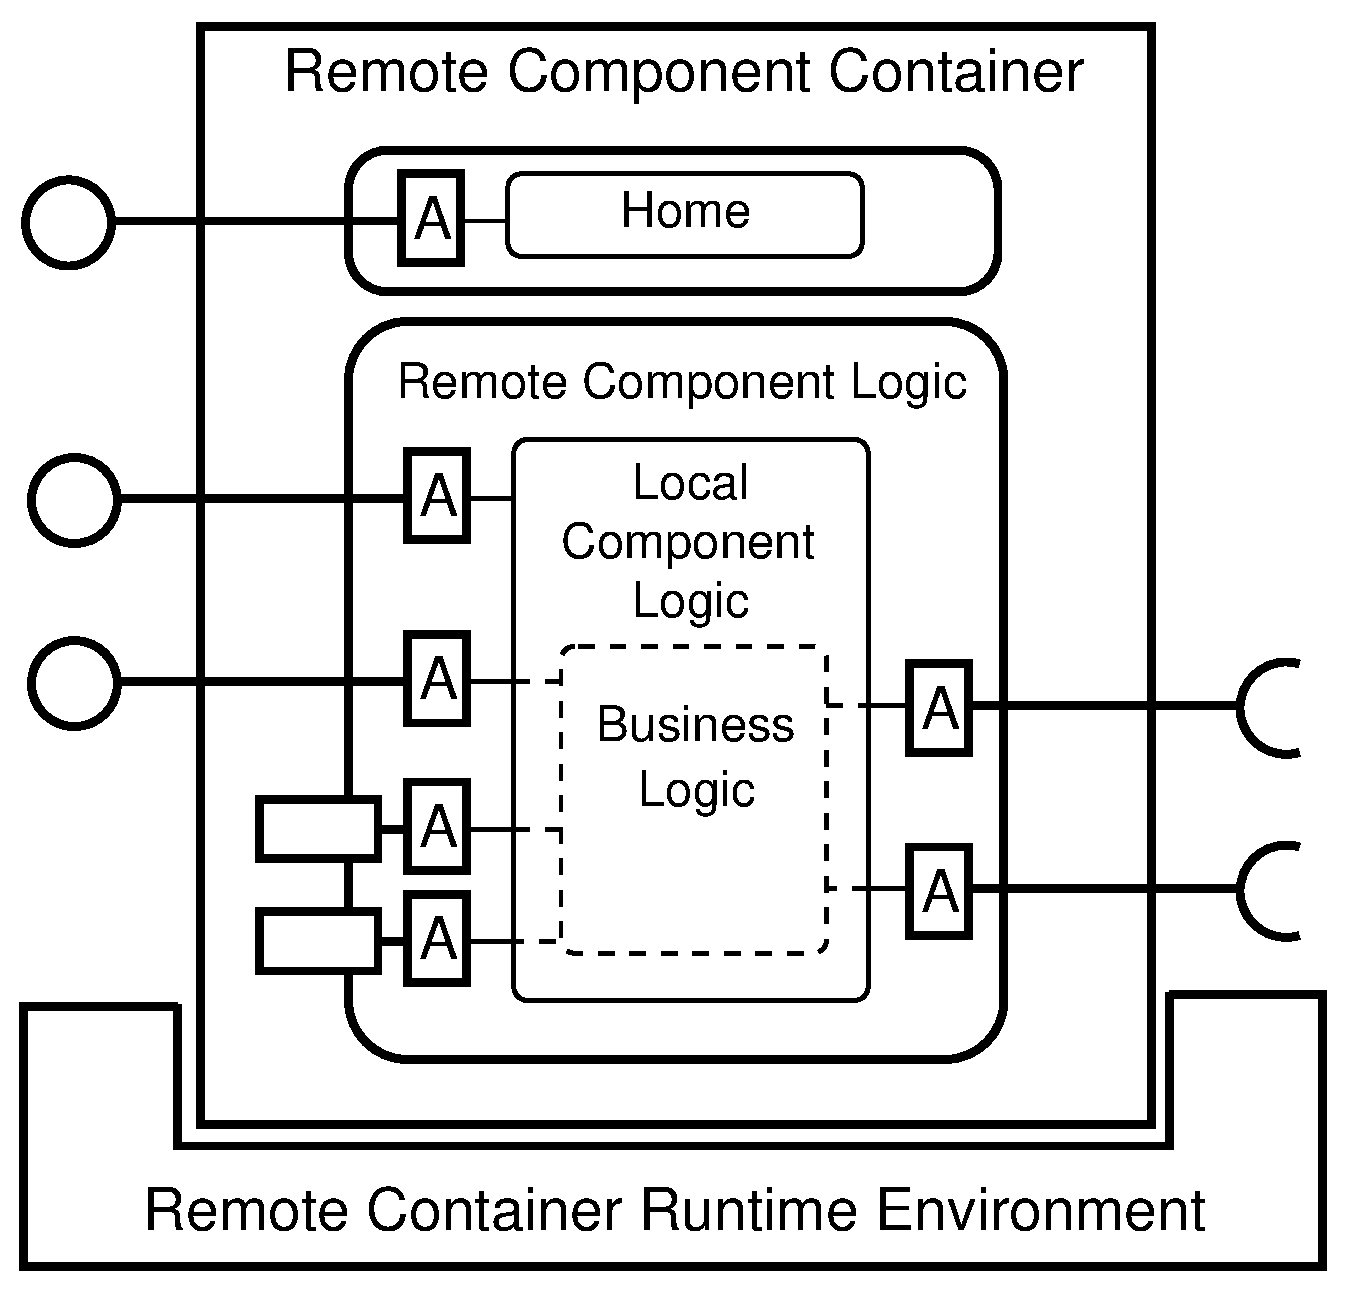
\includegraphics[width=55mm]{figures/LocalAdapterConcept.eps}}

\vspace{30mm}

{\Huge CCM Tools Tutorial}\\ 

\vspace{30mm}

{\Large
\bf
Version: 0.5.1
}\\
(June 5, 2005)
\end{titlepage}
\cleardoublepage


\pagenumbering{roman}
\tableofcontents
%\listoffigures

\cleardoublepage
\pagenumbering{arabic}
\setlength{\parskip}{1em}

%******************************************************************************
\chapter{Introduction}
\label{chapter:introduction}
%******************************************************************************

The CCM Tools are a set of programs and libraries used to generate, package and
deploy CORBA components. The tools implement parts of the CCM specification
\cite{CCMSpecification} with some extensions to improve the usability and
performance of the component model. The {\it CCM Tools User's Guide\/} provides
instructions for using the CCM Tools. This document, the {\it CCM Tools
Developer's Manual\/}, is aimed at developers and provides details on the inner
workings of the CCM Tools.

\begin{figure}
\centering \includegraphics[width=14cm]{ToolsOverview}
\caption{Parts of the CCM Tools package.}
\label{fig:intro-ToolsOverview}
\end{figure}

To help the component developer, the CCM Tools provide the tools shown in
Figure~\ref{fig:intro-ToolsOverview}. These tools include the following parts:

\paragraph{CCM Metamodel Library}

The CCM specification defines a metamodel for the IDL3 syntax. This metamodel is
a set of classes that are capable of representing the syntactic elements in
IDL3. We implemented a metamodel library in Java that allows creation of, and
navigation through, CCM models. Using this library we can clearly separate the
parser and the code generators, using a CCM model as the communication between
the two parts. The parser creates a model object for every part of the source
code matching an IDL grammar rule, and the generator tools read the model to
generate code. Chapter~\cite{chapter:ccm-metamodel-library} describes the CCM
Tools' construction of the CCM metamodel library.

\paragraph{IDL3 Parser}

The IDL3 Parser reads an IDL3 file, checks the syntax of the IDL source code and
creates a CCM model, using the CCM metamodel library, in memory. This CCM model
is the starting point for all code generator tools.
Chapter~\cite{chapter:idl3-parser} describes the IDL3 parser in detail.

\paragraph{Mirror Component Generators}

After building a component it is a good idea to run a set of functional tests on
it. Such testing can provide helpful component specific debugging and prevent
large, difficult to locate, system bugs later in development.

To provide a test environment for every component, the CCM Tools can create a
mirror component (a facet becomes a receptacle and vice versa) described in a
mirror IDL3 file. We use the C++ component generators with the mirror IDL3 files
to generate the code for mirror components. Then we use a C++ mirror test
generator to create a basic test executable that connects each component with
its mirror and calls the functions available for each component.

\paragraph{IDL2 Generator}

To implement CORBA components, IDL3 source code needs to be reduced to IDL2,
which can be interpreted by classic IDL compilers. The transformation from IDL3
to IDL2 also adds some operations needed for navigation between components and
their ports (equivalent operations). The CCM Tools support this transformation
using an IDL2 generator tool that creates IDL2 code based on a CCM model.

\paragraph{Component Descriptor Generator}

To describe the component for the deployment and assembling processes, the OMG
defines a {\it CORBA Component Descriptor} (CCD) file. This is an XML file
containing a short description of a component and its ports. We map the CCM
model to an XML--DOM tree that can be written as an XML file. The CCD file is
also used by the code generators to get some additional information about the
components being generated (version, vendor, etc.).

\paragraph{Local C++ Component Generator}

The CCM Tools include a generator tool that creates the local component logic
from a given CCM model. The generated code contains C++ implementations of a
component that can run in the same address space (hence called a `local
component'). This implementation includes operations for providing, using,
connecting, and disconnecting components and their facets. These generated
operations are referred to as {\bf component logic}. After generating the
component logic, the component developer needs to write the {\bf business
logic}; that is, the functional implementation of the component so that it
becomes useful in a component based software system. See
Chapter~\cite{chapter:component-generator-tools} for more information about the
component generator library.

\paragraph{Remote C++ Component Generator}

Note that the local components can only be used in a common address space and
must be implemented in the same programming language. To overcome these
limitations, the CCM Tools have a remote component generator that produces C++
code to interface the local components with CORBA. The remote component logic is
thus a superset of the local component logic.

\paragraph{UML Parser}

Optionally, the description of the component's interfaces can be contained in a
UML diagram. We need a UML parser that reads the UML--XMI file, builds a UML
model (based on the UML metamodel defined by the OMG) and transposes the model
to a standard IDL3 file. The CCM Tools can use the NSUML UML metamodel library
from NovoSoft, but the OMG has not yet defined an UML profile for the CCM. Thus
a UML tool will likely be on the back burner for some time.

\paragraph{Component Packaging Tool}

After generating and writing the component logic and the component descriptor
file, we have to package these files into a zip file called, predictably, a
component package. The component packaging tool provides these functionalities
to the component developer.

\paragraph{Component Deployment Tool}

On the target host the component package must be unzipped and the component must
be deployed in the application server. The component deployment tool provides
these functionalities to the component deployer.

\section{Assembly tools}

After creating the component logic and writing the business logic, we can use
the component from a simple client program. A big advantage of the CORBA
component model is the ability to connect components together to form larger
structures called {\bf component assemblies}.

A component assembly is a set of components (with their component descriptors)
and a {\it Component Assembly Descriptor} (CAD). Based on the CAD we can
generate an assembly object that instantiates components and connects them
together to form a component assembly.

\begin{figure}
\includegraphics[width=14cm]{AssemblyTools}
\caption{CCM component assembly tools.}
\label{fig:intro-AssemblyTools}
\end{figure}

Figure~\ref{fig:intro-AssemblyTools} provides a diagram of the assembly tools in
the CCM Tools. These tools include:

\paragraph{Assembly Descriptor Generator}

The component descriptor files are the base for the higher--level assembly
descriptor, which describes the components of the assembly and their
connections. That means that all information of the assembly descriptor comes
from the component descriptors of the related components (and some additional
data from a GUI).

\paragraph{Assembly Object Generator}

At runtime a managing object is needed that can establish an assembly instance.
The assembly object creates the component instances and connects their
receptacles and facets. All information for generating an assembly object comes
from the assembly descriptor (or its DOM model in memory). Note that this object
must eventually be able to create local or local/remote assembly instances.

\paragraph{UML Parser}

As with components, there should be a way to define component assemblies in a
UML diagram. Therefore we need a UML parser that reads the UML--XMI file and
translates the data into the DOM model used by the assembly descriptor. The OMG
has not yet defined a mapping between UML and CCM assemblies.

\paragraph{Assembly Packaging Tool}

After generating the component assembly and its descriptor file we have to
package these files into a zip file called a component assembly package. The
assembly packaging tool provides these functionalities to the assembly
developer.

\paragraph{Assembly Deployment Tool}

On the target host the component assembly package must be unzipped and the
assembly must be deployed in the application server. The assembly deployment
tool provides these functionalities to the assembly deployer.

\section{Testing}

Another important issue is {\bf testing}. We have to test our applications on
different levels during development, as listed below:

\paragraph{Class Level Testing}

Every class of the business logic that will be part of a component has to be
tested.

\paragraph{Component Level Testing}

For every component we create a counter component that looks like a mirror to
the original component. This counter component has an receptacle for every facet
of the original component and vice versa. Connecting a component with its mirror
component with a simple test client allows component developers to quickly
isolate component level errors in the business code.

\paragraph{Assembly Level Testing}

After testing each component, we have to be sure that a set of connected
components, the component assembly, also works correctly.

Of course, there must be tool support for testing on these different levels of
development to make this job more efficient.


% $Id$
%==============================================================================
\chapter{Component Development}
%==============================================================================

blah \dots

%Before you start with component development, make sure that the CCM Tools are
%installed in a proper way.


\newpage
% $Id$
%==============================================================================
\section{Hello World Component}
\label{HelloWorldComponent}
%==============================================================================

As a quick tour through CCM Tools, we implement a simple Hello World 
component example (Fig.~\ref{fig:uml-helloworld}). 
Each development step and developer role will be described 
in more detail in one of the next sections, here we give a general overview.

\begin{figure}[htb]
    \begin{center}
        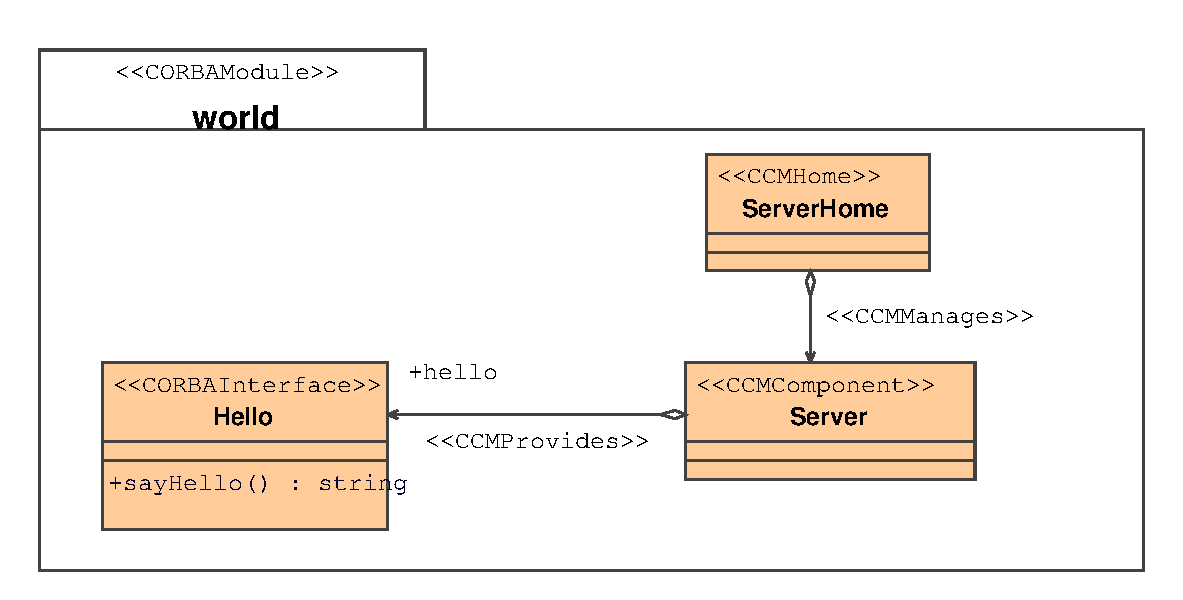
\includegraphics [width=12cm,angle=0] {uml/Hello.eps}
        \caption{A simple HelloWorld component example.}
        \label{fig:uml-helloworld}
    \end{center}
\end{figure}

\vspace{3mm}
\noindent
{\bf Step 1:} We define a component using the 
{\it Interface Definition Language} (IDL). 
This simple component only provides a single interface containing a single
method. Don't forget to define a home for this component type.
The following IDL definitions are stored in
a file called {\tt Hello.idl}:
\begin{small}
\begin{verbatim}
module world
{ 
    interface Hello 
    { 
        string sayHello(); 
    }; 

    component Server 
    { 
        provides Hello hello;
    }; 

    home ServerHome manages Server
    {
    };
};
\end{verbatim}
\end{small}


\noindent
{\bf Step 2:} Generate a uniform IDL3 structure from the single {\tt Hello.idl}
file:
\begin{small}
\begin{verbatim}
> ccmtools idl3 -o server/idl Hello.idl
\end{verbatim}
\end{small}

\noindent
This uniform IDL3 structure separates between interfaces (including 
parameter type and exception definitions) and components (including their
homes). Such a separation makes sense because an interface can be used by
many component definitions.
\begin{small}
\begin{verbatim}
    server/
     |-- idl
     |   |-- component
     |   |   `-- world
     |   |       |-- Server.idl
     |   |       `-- ServerHome.idl
     |   `-- interface
     |       `-- world
     |           `-- Hello.idl
\end{verbatim}
\end{small}


\noindent
{\bf Step 3:} Generate an empty component skeleton from the uniform IDL3 
structure:
\begin{small}
\begin{verbatim}
> ccmtools c++local -o server/interface \
                    -Iserver/idl/interface \
                    -Iserver/idl/component \
                    server/idl/interface/world/*.idl

> ccmtools c++local -a -o server/component/Server \ 
                    -Iserver/idl/interface \
                    -Iserver/idl/component \
                    server/idl/component/world/Server*.idl  
\end{verbatim}
\end{small}

\noindent
CCM Tools generate the following file structure which represents a local
component's implementation.
Code contained in the {\tt CCM\_*} directories establishes the component's
structure (= {\it component logic}), while code stored in the {\tt Server} 
directory represents the functional part of a component (= {\it business
logic}).

\begin{small}
\begin{verbatim}
   server
    |-- idl
    |-- component
    |   `-- Server
    |       |-- CCM_world_ccm_local_component_Server
    |       |-- CCM_world_ccm_local_component_Server_share
    |       |-- Makefile.py
    |       |-- ServerHome_impl.cc
    |       |-- ServerHome_impl.h
    |       |-- Server_hello_impl.cc
    |       |-- Server_hello_impl.h
    |       |-- Server_impl.cc
    |       |-- Server_impl.h
    |       `-- world_ccm_local_component_Server_ServerHome_entry.h
    `-- interface
        |-- CCM_world_ccm_local
        `-- CCM_world_ccm_local_adapter
\end{verbatim}
\end{small}

\noindent
{\bf Step 4:} Implement the component's business logic.
The component's business logic must be embedded in the generated
component logic. 
To implement the {\tt sayHello()} method of the {\tt Hello} interface,
we extend the generated {\tt Server\_hello\_impl.cc} file:
\begin{small}
\begin{verbatim}
std::string
hello_impl::sayHello()
    throw(::ccm::local::Components::CCMException)
{
    // TODO : IMPLEMENT ME HERE !
    return "Hello from Server component!";
}
\end{verbatim}
\end{small}

\noindent
Additionally, we create some {\tt Makefile.py} files which tell
{\tt confix} which package name, version and subdirectories
should be used.
\begin{small}
\begin{verbatim}
# server/Makefile.py
PACKAGE_NAME('HelloWorld')
PACKAGE_VERSION('1.0.0')
\end{verbatim}
\end{small}

\begin{small}
\begin{verbatim}
> touch server/interface/Makefile.py
> touch server/component/Makefile.py
> touch server/component/Server/Makefile.py
\end{verbatim}
\end{small}

\noindent
To compile and install this component, simply type: 
\begin{small}
\begin{verbatim}
> confix.py --packageroot=`pwd`/server --bootstrap --configure \
            --make --targets=install
\end{verbatim}
\end{small}


\noindent
{\bf Step 5:} Now we can implement a client that uses the Hello World
component. For this simple case, we implement the client as a {\tt \_check*}
file that will be automatically executed from a {\tt make check} command.

\begin{small}
\begin{verbatim}
   client/
   |-- Makefile.py
   `-- _check_client.cc
\end{verbatim}
\end{small}

\noindent
The following client code snippets are stored in the 
{\tt client/\_check\_client.cc} file:
\begin{small}
\begin{verbatim}
#include <WX/Utils/debug.h>
#include <WX/Utils/smartptr.h>

#include <ccm/local/Components/CCM.h>
#include <ccm/local/HomeFinder.h>

#include <world/ccm/local/component/Server/Server_gen.h>
#include <world/ccm/local/component/Server/ServerHome_gen.h>

using namespace std;
using namespace WX::Utils;
using namespace world::ccm::local;

int main(int argc, char *argv[])
{
    SmartPtr<component::Server::Server> server;
    SmartPtr<Hello> hello;
    ccm::local::Components::HomeFinder* homeFinder =
      ccm::local::HomeFinder::Instance();
    int error;

    try {

      // Deploy component type
      error = deploy_world_ccm_local_component_Server_ServerHome("ServerHome");
      if(error) {
        cerr << "BOOTSTRAP ERROR: Can't deploy component homes!" << endl;
        return(error);
      }
      
      // Instantiate component
      SmartPtr<component::Server::ServerHome> 
          home(dynamic_cast<component::Server::ServerHome*>
          (homeFinder->find_home_by_name("ServerHome").ptr()));
      server = home->create();   
      hello = server->provide_hello();
      server->configuration_complete();
    
      // Use component instance
      string s = hello->sayHello();
      cout << "sayHello(): " << s << endl;

      // Destroy component instance
      server->remove();

      // Undeploy component type
      error += undeploy_world_ccm_local_component_Server_ServerHome("ServerHome");
      if(error) {
        cerr << "ERROR: Can't undeploy component homes!" << endl;
        return(error);
      }
    } 
    catch ( ccm::local::Components::HomeNotFound ) {
        cout << "ERROR: can't find a home!" << endl;
        error = -1;
    } 
    catch ( ccm::local::Components::NotImplemented& e ) {
        cout << "ERROR: function not implemented: " 
	     << e.what (  ) << endl;
        error = -1;
    }  
    catch ( ccm::local::Components::InvalidName& e ) {
        cout << "ERROR: invalid name during connection: " 
             << e.what (  ) << endl;
        error = -1;
    }

    // Clean up singleton
    ccm::local::HomeFinder::destroy();
}
\end{verbatim}
\end{small}


\noindent
Again, we write a {\tt client/Makefile.py} that tells {\tt confix} the
name and version of the client package.
\begin{small}
\begin{verbatim}
PACKAGE_NAME('HelloClient')
PACKAGE_VERSION('1.0.0')
\end{verbatim}
\end{small}

\noindent
To compile and run the component's client, type the following {\tt confix}
line: 
\begin{small}
\begin{verbatim}
> confix.py --packageroot=`pwd`/client --bootstrap --configure \
            --make --targets=check
\end{verbatim}
\end{small}

\noindent
After all, we are happy to see the following output at the end of the client's
build process:

\begin{small}
\begin{verbatim}
sayHello(): Hello from Server component!
PASS: hello-client__check_client
==================
All 1 tests passed
==================
\end{verbatim}
\end{small}

\noindent
Of course, to implement a component for a simple 'Hello from Server component!'
message is somewhat academical, but this example shows how simple a component
development cycle can be. 
The intent of this section was to define the main activities in component 
development, which are:
\begin{itemize}
\item Define a component's structure (using IDL or UML).
\item Generate an empty component skeleton (called component logic).
\item Implement a component's business logic. 
\item Implement a component's client.
\end{itemize}

\noindent
In the following sections, we will explore each of these steps in more
detail. However, keep this big picture in mind. 


\newpage
% $Id$
%==============================================================================
\section{A Local Component's Structure}
\label{ComponentStructure}
%==============================================================================

The implementation of server--side components is made up of different parts,
as shown in Fig.~\ref{ContainerComponentlogicBusinesslogic}, that are either
manually written, generated by tools or existing libraries.

\begin{figure}[htbp]
    \begin{center}
    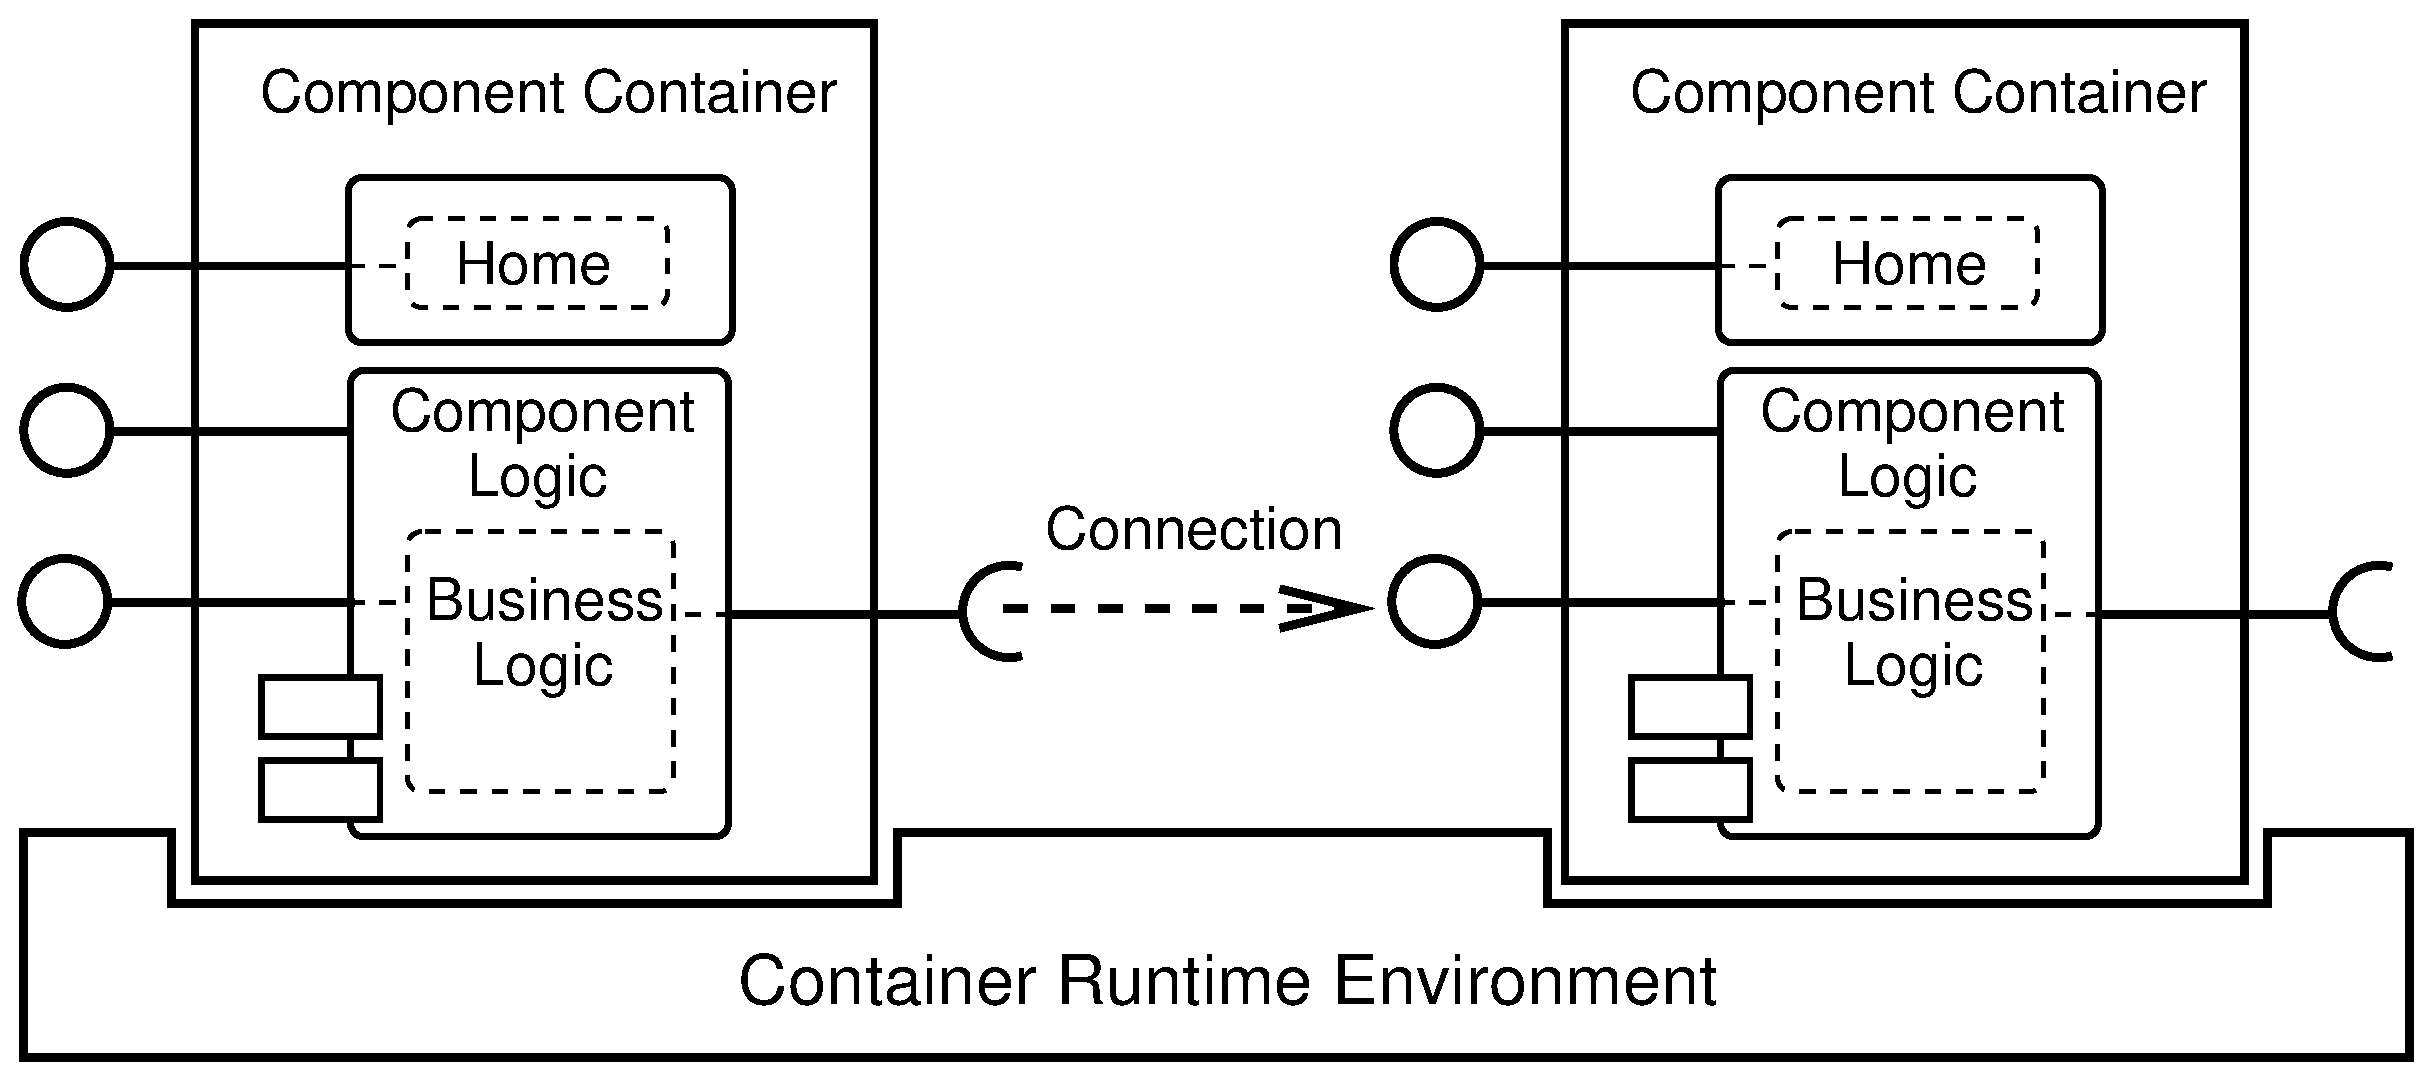
\includegraphics [width=10cm,angle=0] 
		     {figures/ContainerComponentlogicBusinesslogic.eps}
    \caption{A component implementation covers business logic, component
    logic, component container and container runtime environment.}
    \label{ContainerComponentlogicBusinesslogic}            
    \end{center}
\end{figure}

\begin{description}
\item [Business logic:]
  a component's business logic is written by the component developer to 
  implement   a domain specific functionality.
  Basically, business logic should not deal with technical aspects like contract
  verification or middleware API.
  
\item [Component logic:]
  business logic is embedded in a layer of generated code called component 
  logic. The interaction between business logic and component logic is well 
  defined in terms of interfaces (context interface, callback interface).
  Component logic handles technical aspects as well as a component's life-cycle.
  Additionally, component logic is glue code that fits a component into a 
  generic component container.
  
\item [Component container:]
  a component type is hosted by a component container that manages instances of
  that component type.
  While component logic is generated for each particular component type, the 
  component container is a generic part of the component platform.
  
\item [Container runtime environment:]
  a component platform also supports a set of libraries and services that can 
  be used by component containers.
  Any middleware used here is also part of this runtime environment.
\end{description}


\noindent
From this implementation schema, two different component views can be deduced:
\begin{description}
\item [External view:]
  a component provides its ports defined by interfaces. All 
  client calls to these ports are routed through the component container and 
  the generated component logic before business logic functionality is
  executed.
  
\item [Internal view:]
  a component's business logic can call methods on a context 
  object, which is part of generated component logic, and has to implement 
  a callback interface that allows the component container to handle the 
  component's life--cycle.
\end{description}


\noindent
Conforming with the concept of component model and 
middleware separation, we have implemented a local version of LwCCM components.
These local components host business logic and are completely independent 
from a particular middleware technology.

\begin{figure}[htbp]
    \begin{center}
    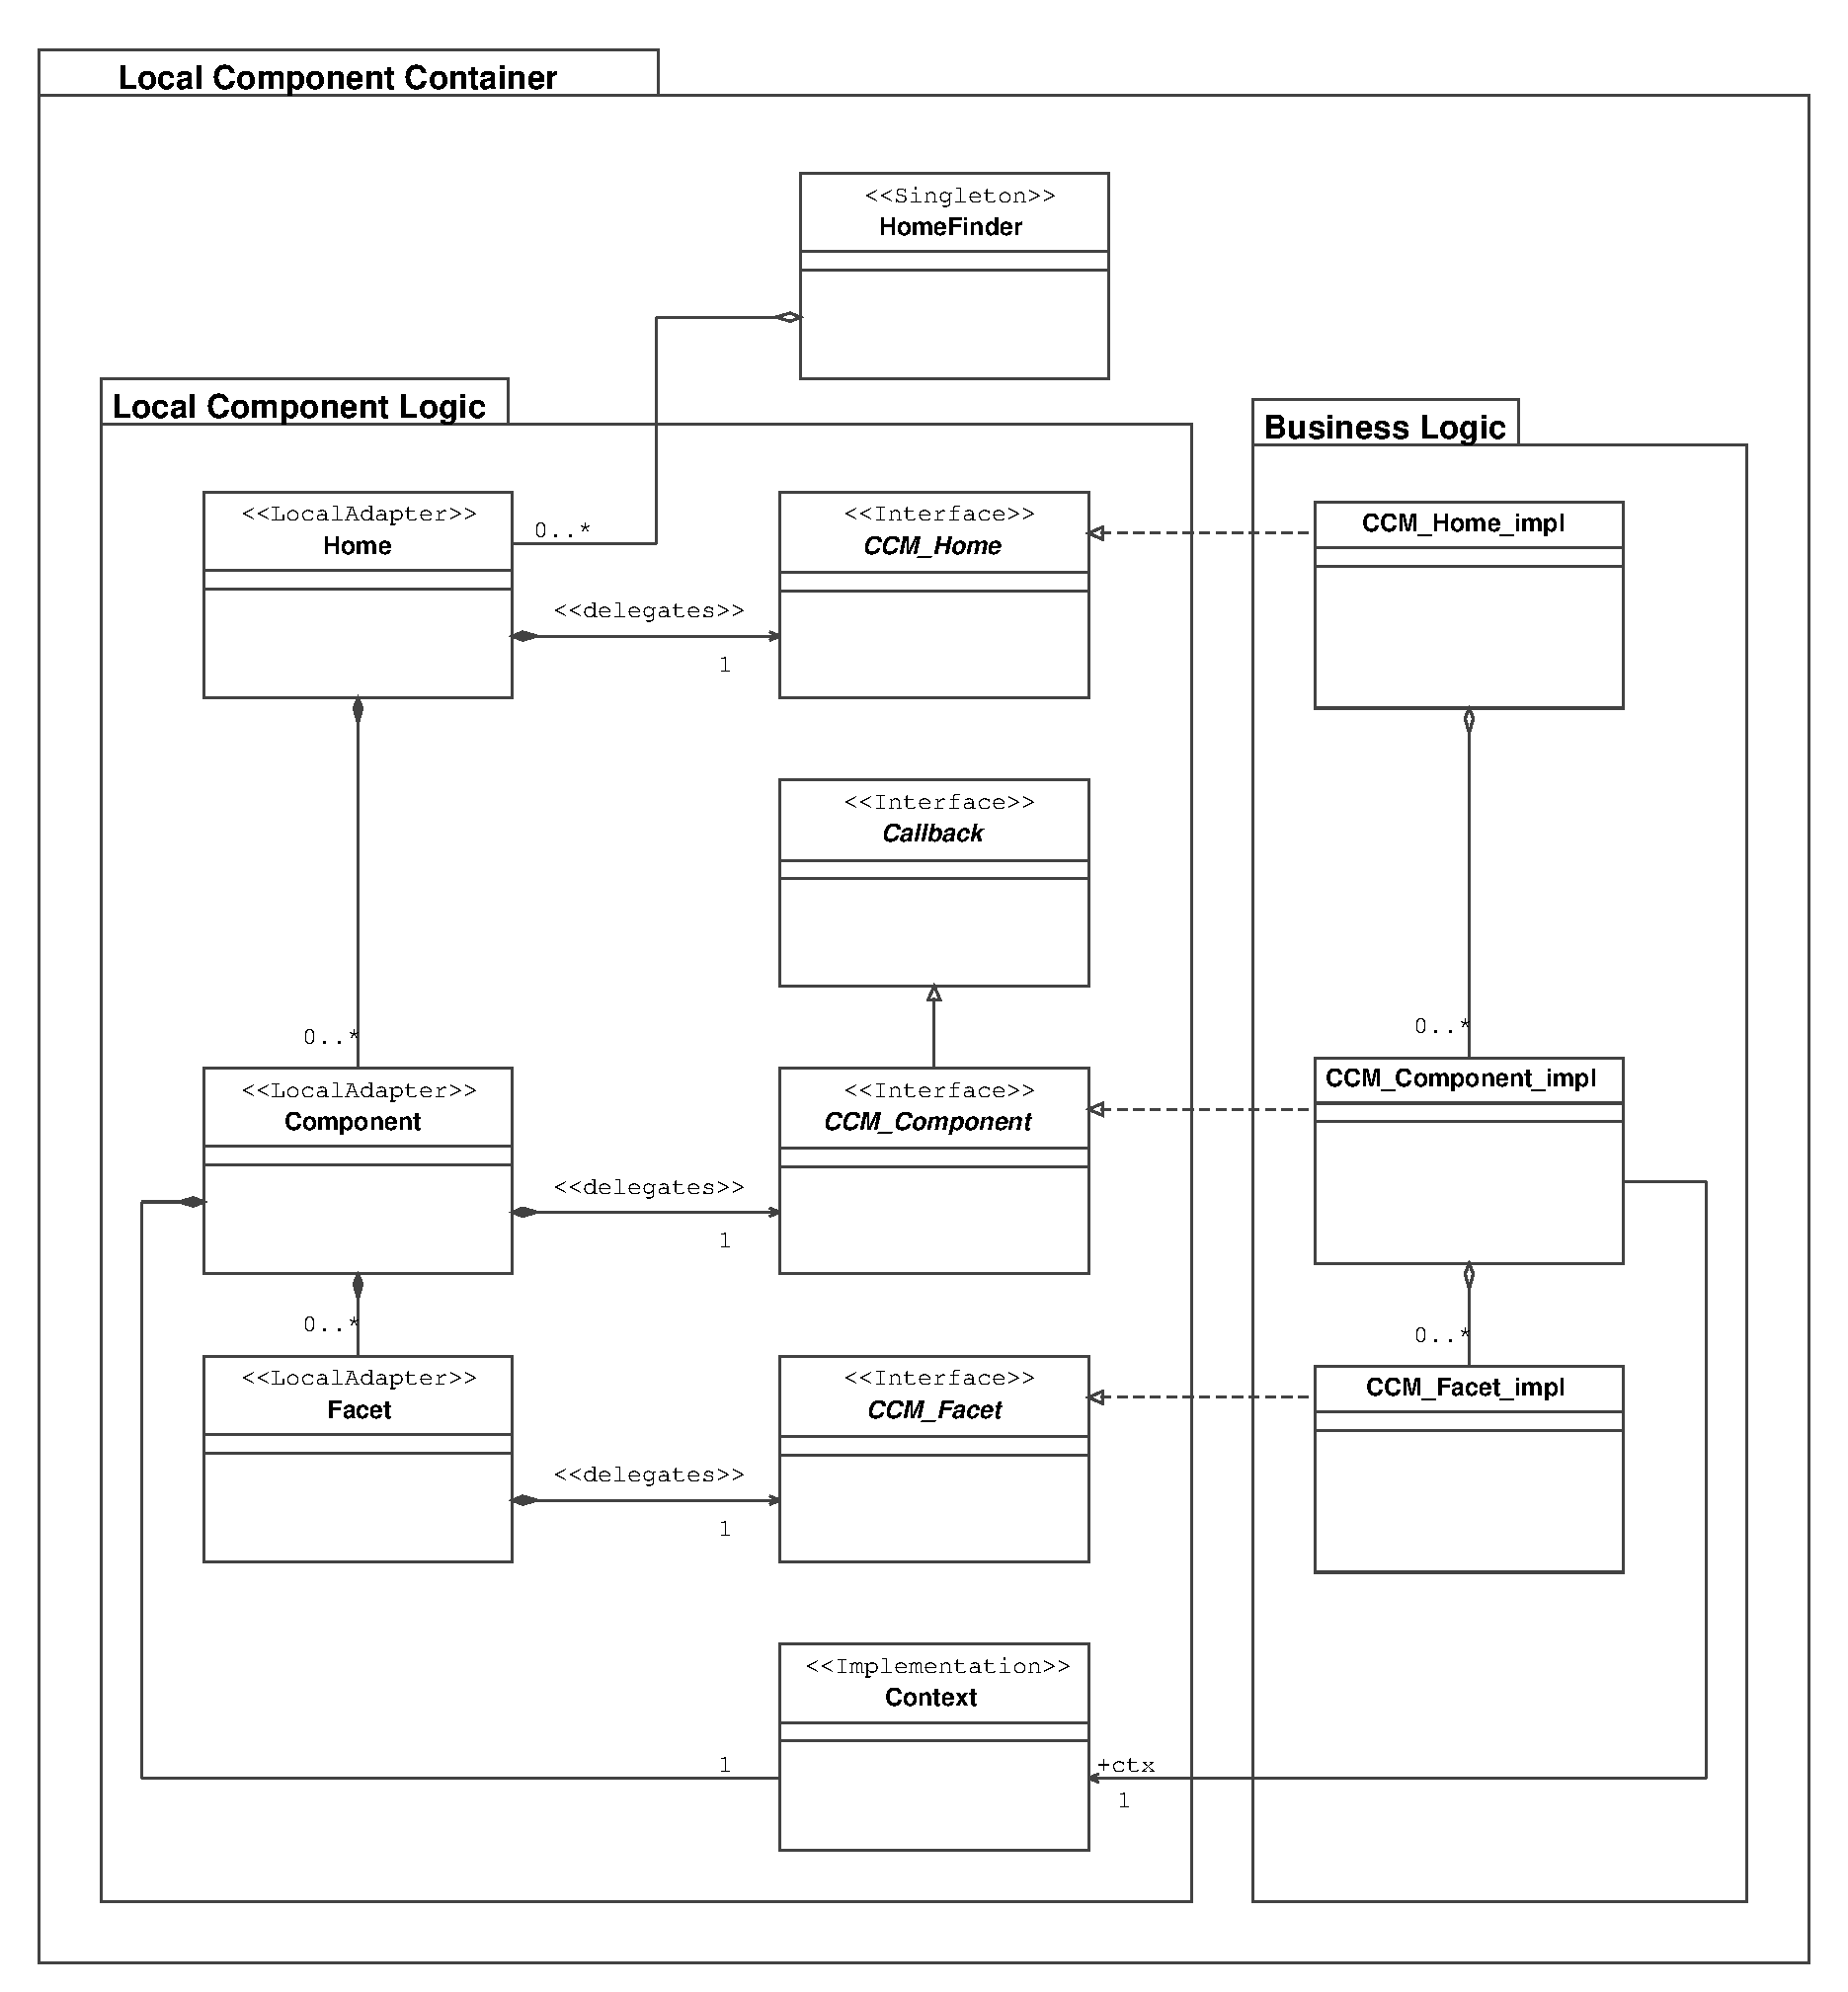
\includegraphics [width=15cm,angle=0] {uml/StructureOfLocalComponents.eps}
    \caption{This simplified structure of a local component implementation
    shows the relationship between business logic, local component logic and
    a local component container.}
    \label{StructureOfLocalComponents}            
    \end{center}
\end{figure}

\noindent
Implementations without middleware are much leaner and allow
finer grained components which are simpler to reuse.
Especially in languages that do not provide a native component model
(like C++), a local version of LwCCM can be useful.  

\newpage
\noindent
Based on this simplified class diagram, we can analyze the following
interactions between business logic and component logic:

\begin{description}
\item [Calling component methods:]
usually, a component client calls methods on a component's interface.
These interfaces can be either a component home, a component equivalent 
interface or a facet.
Invocations on all these interfaces follow the same structural pattern,
as shown in Fig.~\ref{LocalComponentImplementationStructure}.
A component's client calls methods on generated adapter classes 
that implements a component's interfaces. 
These adapters delegate calls 
to generated interfaces which are implemented by business logic classes.
\begin{figure}[htbp]
    \begin{center}
    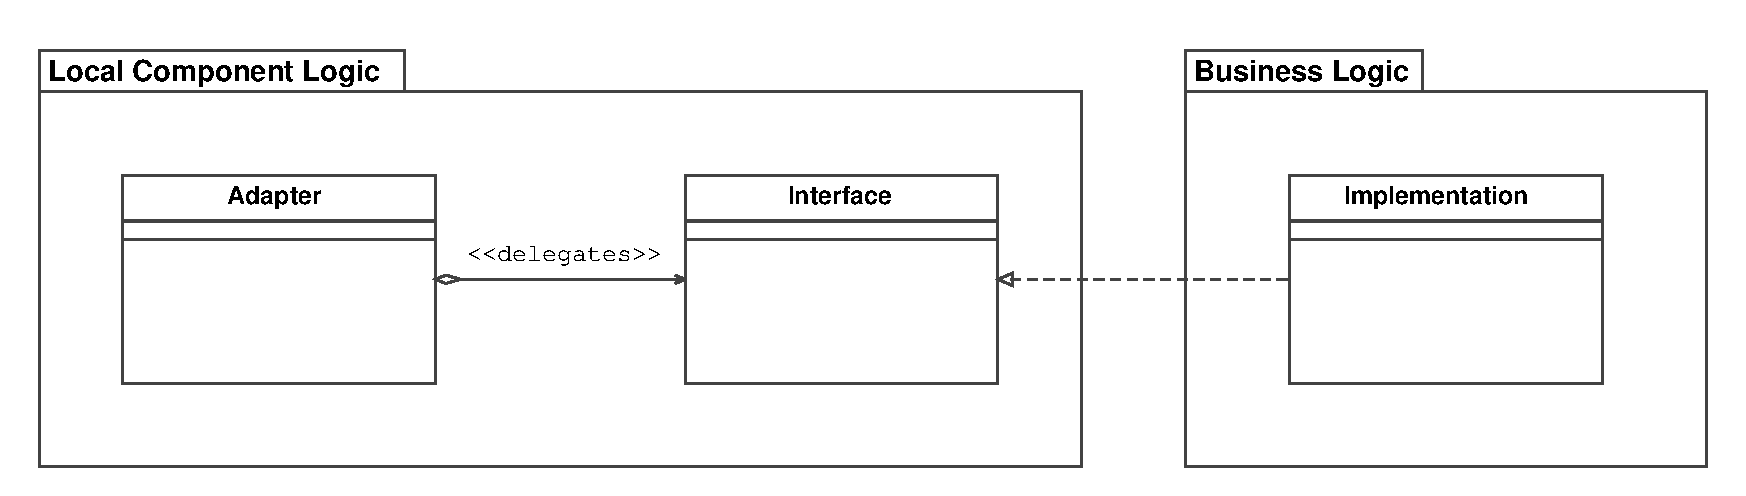
\includegraphics [width=13cm,angle=0] 
		     {uml/LocalComponentImplementationStructure.eps}
    \caption{Structure of a local component.}
    \label{LocalComponentImplementationStructure}            
    \end{center}
\end{figure}

This pattern implies two benefits:
\begin{itemize}
\item The adapter layer brings in an indirection that can be used to execute
some pre- and post-invocation functionality.  

\item Business logic can implement a well defined interface which is generated 
from the component model.
\end{itemize}

\item [Invoking callback methods:]
as shown in Fig.~\ref{StructureOfLocalComponents}, a generated component 
interface inherits the {\tt Callback} interface that defines methods which 
will be used by the component logic to control the business logic life-cycle.

\item [Using context methods:]
while calls from component clients as well as calls from component logic to 
the callback interface 
are directed from outside to the business logic, there is also
a need for interaction between business logic and generated glue code.

In the other direction, from business logic to component logic, a {\tt Context}
object is used to provide access to container functionality.
Additionally, business logic gets receptacle references from this context 
object, that are used to call methods defined by these receptacle interfaces.
Remember, receptacles are connected to facets which implement these common
interfaces.
\end{description}

\noindent
An important part of a local component container is the {\tt HomeFinder} class. 
This class is implemented as a singleton
\cite{Gamma95} and manages component home instances.
When a local LwCCM component is deployed, an instance of the component's home
is created and registered by the {\tt HomeFinder} using a unique name. 
After that, the {\tt HomeFinder} can be used to retrieve home references by 
their name.

\newpage
% $Id$
%==============================================================================
\section{Test--Driven Component Development}
\label{TestDrivenComponentDevelopment}
%==============================================================================

As we have seen from the Hello World example, components can be implemented in
a parallel task.
While system design describes the structure and interactions between 
components, component implementation constitutes the components behavior.

%------------------------------------------------------------------------------
\subsection{Component development process}
%------------------------------------------------------------------------------
The component development process defines activities needed to 
implement a component's business logic embedded in a generated 
component logic in a test--driven approach. 
Fig.~\ref{ProcessComponentDevelopment} shows the {\it write the test first}
paradigm used in test--driven component development.

\begin{figure}[htbp]
    \begin{center}
    \includegraphics [width=4.5cm,angle=0] {figures/ProcessComponentDevelopment.eps}
    \caption{A test--driven component development process.}
    \label{ProcessComponentDevelopment}            
    \end{center}
\end{figure}

\noindent
Two nested iteration cycles are shown in the diagram 
(Fig.~\ref{ProcessComponentDevelopment}). 
The inner iteration cycle 
is concerned with implementing and testing business logic to pass a particular 
test case.
The outer iteration cycle is started with every new test case derived from a 
functional requirement analysis.

\newpage
\noindent
The presented component development process contains the following activities: 
\begin{itemize}
\item {\bf Generate component.}
Based on component descriptions, tools can be used to 
generate platform specific component logic which can host the implemented 
business logic.

\item {\bf Analyze requirements.}
A component has to satisfy a set of functional requirements. The description 
of these requirements can be formally specified, modeled or written in prosa.

\item {\bf Implement test cases.}
From the requirements specifications, test cases can be implemented. 
These test cases express a component's usage in a particular programming 
language.
There will be a test case for every postulated aspect of the component's 
functionality.
Each executable test case augments the set of automated tests that can be
run again later for regression testing too.

\item {\bf Implement business logic.}
The business logic must be implemented in a way that the implemented test cases
can run without a failure. 
There is no need for a component developer to know the overall goal of the 
software system. 
The business logic is only determined by requirements expressed by executable
test cases.

\item {\bf Run test case.}
At every time in development, the business logic of a component can be checked
by running all implemented test cases.
Thus, there is a well defined end to component development - as soon as all 
test cases, that represents the functional requirements, are
running, the work is done.
\end{itemize}

\noindent
The fact, that each implementation of a component's functionality starts by 
writing a test case, automatically leads to testable business logic.
Another benefit of executable test cases is that - after a change in 
business code - the whole test suite can be run to ensure the functional 
integrity of the component's implementation. 


%------------------------------------------------------------------------------
\subsubsection{Component development roles}
%------------------------------------------------------------------------------
The test--driven component development process defines two development roles 
which are usually performed by the same person:

\begin{itemize}
\item {\bf Test developer.}
A test developer analyzes the functional requirements for a component's 
business logic and implements test cases that can verify these requirements 
automatically.
 
\item {\bf Component developer.}
A component developer implements a component's business logic in respect to the
given test cases. His work is done, when all tests run through. 
\end{itemize}


\newpage
%------------------------------------------------------------------------------
\subsection{Car rental example}
%------------------------------------------------------------------------------

As a simple example, we define a car rental component that can handle customers
and miles. For each customer we can evaluate driven miles and costs incurred. 
We will store all created IDL files in a {\tt CarRental} directory
\footnote
{
You can find this example source code in the 
{\tt ccmtools/test/tutorial/CarRental} directory.}:
\begin{small}
\begin{verbatim}
        CarRental/
        |-- Exceptions.idl
        |-- Customer.idl
        |-- CustomerMaintenance.idl
        |-- CustomerBusiness.idl
        `-- CarRental.idl
\end{verbatim}
\end{small}

Keep in mind that IDL files contain no specification of what exact action will 
be performed.
The component developer bears the responsibility of filling in the functionality
after the component logic has been generated.

\begin{small}
\begin{verbatim}
#ifndef __EXCEPTIONS_IDL__
#define __EXCEPTIONS_IDL__

module BigBusiness {
  exception CreateCustomerException{};
  exception RemoveCustomerException{};
  exception NoCustomerException{};
}; // End of module BigBusiness
#endif
\end{verbatim}
\end{small}
This first code snippet shows the definition of three IDL exceptions.
In order to get a namespace, we envelop these definitions using a module called 
{\tt BigBusiness}. 
To prevent IDL files from multiple including, we define {\it include guards} 
within each source file.



 
\begin{small}
\begin{verbatim}
#ifndef __CUSTOMER_IDL__
#define __CUSTOMER_IDL__

module BigBusiness {
  struct Customer {
    long id;
    string first_name;
    string last_name;
    double mileage;
  };
  typedef sequence<Customer> CustomerList;
}; // End of module BigBusiness
#endif
\end{verbatim}
\end{small}

In {\tt Customer.idl}, we define a structure of basic data types and a sequence 
of this structure type.
Again, there is a {\tt BigBusiness} module and an include guard.

\begin{small}
\begin{verbatim}
#ifndef __CUSTOMER_MAINTENANCE_IDL__
#define __CUSTOMER_MAINTENANCE_IDL__

#include"Exceptions.idl"
#include"Customer.idl"

module BigBusiness {
  interface CustomerMaintenance
  {
    void createCustomer(in Customer person) 
      raises (CreateCustomerException);
    Customer retrieveCustomer(in long id)  
      raises (NoCustomerException);
    CustomerList retrieveAllCustomers()  
      raises (NoCustomerException);
    void updateCustomer(in Customer person)  
      raises (NoCustomerException);
    void deleteCustomer(in long id)  
      raises (RemoveCustomerException);
  };
}; // End of module BigBusiness
#endif
\end{verbatim}
\end{small}
Customers must be handled in a database like way. 
Thus, {\tt CustomerMaintenance.idl} contains a 
{\it Create, Retrieve, Update and Delete} (CRUD) interface. 
To pick a particular {\tt Customer}, we use a customer id that is realized by 
an IDL long type.
Methods can throw exceptions in the case of illegal customer ids, create or 
remove problems. 


\begin{small}
\begin{verbatim}
#ifndef __CUSTOMER_BUSINESS_IDL__
#define __CUSTOMER_BUSINESS_IDL__

#include "Exceptions.idl"

module BigBusiness {
  interface CustomerBusiness
  {
    attribute double dollars_per_mile;
    void addCustomerMiles(in long id, in double miles) 
      raises(NoCustomerException);
    void resetCustomerMiles(in long id) 
      raises(NoCustomerException);
    double getCustomerMiles(in long id) 
      raises(NoCustomerException);
    double getCustomerDollars(in long id) 
      raises(NoCustomerException);
  };
}; // End of module BigBusiness
#endif
\end{verbatim}
\end{small}

Beside the pure data manipulation, we also need an interface that defines a
business functionality.
{\tt CustomerBusiness.idl} defines an attribute and some methods that operate
on the given customer data. 
If a parameter represents a wrong customer id, the {\tt NoCustomerException}
will be thrown.

\begin{small}
\begin{verbatim}
#ifndef __CAR_RENTAL_IDL__
#define __CAR_RENTAL_IDL__

#include "CustomerMaintenance.idl"
#include "CustomerBusiness.idl"

module BigBusiness {

  component CarRental 
  { 
    provides CustomerMaintenance maintenance;
    provides CustomerBusiness business;
  };
  
  home CarRentalHome manages CarRental 
  { };

}; // End of module BigBusiness
#endif
\end{verbatim}
\end{small}

Finally, we collect the included interfaces to a {\tt CarRental} component and 
define a {\tt CarRentalHome} that will be used to create component instances at
runtime.

Well done! We have defined our component in terms of IDL.


\vspace{10mm}
%------------------------------------------------------------------------------
\subsubsection{Generate component}
%------------------------------------------------------------------------------

In this step, we bring the IDL3 files in a proper structure that implies 
the separation between interface and component definitions. 
\begin{small}
\begin{verbatim}
> ccmtools idl3 -o server/idl3 *.idl
\end{verbatim}
\end{small}
A result of this CCM Tools call is the following file structure.
The separation between interface and component related files reflects the
fact that interfaces are used to defined components but are not owned by
these components.
\begin{small}
\begin{verbatim}
server
`-- idl3
    |-- component
    |   `-- BigBusiness
    |       |-- CarRental.idl
    |       `-- CarRentalHome.idl
    `-- interface
        `-- BigBusiness
            |-- CreateCustomerException.idl
            |-- Customer.idl
            |-- CustomerBusiness.idl
            |-- CustomerList.idl
            |-- CustomerMaintenance.idl
            |-- NoCustomerException.idl
            `-- RemoveCustomerException.idl
\end{verbatim}
\end{small}


To generate C++ source code from IDL3 we have to call the CCM Tools generator
twice, once for the interfaces and once for the component:
\begin{small}
\begin{verbatim}
> ccmtools c++local -o server/interface \
                    -Iserver/idl3/interface \
                     server/idl3/interface/BigBusiness/*.idl
> ccmtools c++local -a -o server/component/CarRental \
                    -Iserver/idl3/component \
                    -Iserver/idl3/interface \
                     server/idl3/component/BigBusiness/CarRental*.idl 
\end{verbatim}
\end{small}

Now, the {\tt server} directory contains the component's source code. 
(To get a description of all {\tt ccmtools} options consult the 
CCM Tools commands section in the tutorial's appendix).
\begin{small}
\begin{verbatim}
server
|-- idl3
|-- component
|   `-- CarRental
|       |-- CCM_Local_BigBusiness_CCM_Session_CarRental
|       |-- CCM_Local_BigBusiness_CCM_Session_CarRental_share
|       `-- impl
|           |-- CarRentalHome_entry.h
|           |-- CarRentalHome_impl.cc
|           |-- CarRentalHome_impl.h
|           |-- CarRental_business_impl.cc
|           |-- CarRental_business_impl.h
|           |-- CarRental_impl.cc
|           |-- CarRental_impl.h
|           |-- CarRental_maintenance_impl.cc
|           |-- CarRental_maintenance_impl.h
|           `-- Makefile.py
`-- interface
    `-- CCM_Local_BigBusiness
        |   |-- CreateCustomerException.h
        |   |-- Customer.h
        |   |-- CustomerBusiness.h
        |   |-- CustomerList.h
        |   |-- CustomerMaintenance.h
        |   |-- Makefile.py
        |   |-- NoCustomerException.h
        |   `-- RemoveCustomerException.h
        `-- Makefile.py
\end{verbatim}
\end{small}

The component developer really ought not to care about the generated 
{\tt CCM\_Local\_*} subdirectories (if you don't believe us, though, feel free 
to read through it; just don't edit anything). 
The interesting files are listed in the {\tt impl} directory. 
These files contain skeleton code (that are empty methods) of the component's 
business logic.

\begin{itemize}
\item {\tt CarRentalHome\_entry.h} \\
This file is the business logic's entry point and declares an extern ``C'' 
function that returns a component home instance.
The generated implementation of this function is hosted in the 
{\tt CarRentalHome\_impl.cc} file.

\item {\tt CarRentalHome\_impl.[h,cc]} \\
These files contain the factory methods for component instantiation. 
While user defined factory methods must be implemented manually, the default 
{\tt create} method is already generated.

\item {\tt CarRental\_impl.[h,cc]} \\
These files contain the implementation of supported interfaces as well as the
implementation of component attributes.

\item {\tt CarRental\_business\_impl.[h,cc]} \\
{\tt CarRental\_maintenance\_impl.[h,cc]} \\
These files contain the implementation of defined facets and builds
the component's business logic
(grep for {\tt // TODO : IMPLEMENT ME HERE !}).

\item {\tt Makefile.py} \\
This file is a Confix marker that denotes a directory as 'to compile'.
\end{itemize}

Files in the {\tt impl} directory are protected from overwriting.
Running the generator again results in a bunch of warnings. 
Instead of overwriting, the generator stores the new files with an extension 
({\tt *.new}) into the same directory.
You can make a {\tt diff} to figure out changes. 

\vspace{3mm}
The generated business logic skeletons contains enough code to be compilable.
Confix, our build tool, needs some informations about the package to build.
The following content must be placed in the {\tt server/Makefile.py} file:
\begin{small}
\begin{verbatim}
# server/Makefile.py
PACKAGE_NAME('CarRental')
PACKAGE_VERSION('1.0.0')
\end{verbatim}
\end{small}
Additionally, some empty {\tt Makefile.py} files must be placed in
source directories to force {\tt Confix} to build them:
\begin{small}
\begin{verbatim}
> touch server/interface/Makefile.py
> touch server/component/Makefile.py
> touch server/component/CarRental/Makefile.py
\end{verbatim}
\end{small}

Finally, to build the generated {\tt Carrental} component, type:
\begin{small}
\begin{verbatim}
> confix.py --packageroot=`pwd`/server --bootstrap --configure --make
\end{verbatim}
\end{small}



%------------------------------------------------------------------------------
\subsubsection{Mirror Component Concept (MCC)}
%------------------------------------------------------------------------------

Software development is an iterative process. Kent Beck
has proposed a {\it Test Driven Development} (TDD) methodology 
\cite{Beck2003TDD} that starts by
implementing the test~-- before implementing the business logic!

As shown in Fig.~\ref{fig:test-driven-development}, the CCM Tools make use of
the TDD idea in the context of components. For every component $C$, we
generate a mirror component $\overline{C}$. Each input port (receptacle)
of $C$ corresponds to an output port (facet) of $\overline{C}$, and vice versa.

\begin{figure}[htb]
    \begin{center}
    \includegraphics [width=5cm,angle=0] {figures/TestArchitecture.eps}
    \caption{A Component test architecture consists of a 
      $(C, \overline{C})$ pair that is managed by a test client.}
    \label{fig:test-driven-development}
    \end{center}
\end{figure}

Fig.~\ref{TestClientSequenceDiagramm} shows the sequence diagram for this 
automatic test concept.
Basically, a mirror component test is made up of three execution phases:

\begin{itemize}
\item Setup phase (step 1 to 10): \\
Before a test case can be executed, the mirror component test environment must
be established.
First, both components must be created and configured by their attributes.
$C$ and $C\_mirror$ hold the same attribute set,
thus, both components can be configured in the same way. 
Then, $C$ and $C\_mirror$ are connected with each other.

Calling {\tt configuration\_complete} finishes this build--up phase.

\item Testing phase (step 11):\\
In this phase all test cases implemented in $C\_mirror$ are executed.
Remember, after a {\tt configuration\_complete} call from a client, the 
container calls a component's {\tt ccm\_activate} callback method.
Test cases can be implemented in or called from this callback
method. 
As all test cases are implemented within a component, a test 
developer can use the same programming paradigm as a component developer. 

\item Tear down phase (step 12 to 15): \\
After all test cases have finished, the mirror component test environment must 
be destroyed.
All connections between $C$ and $C\_mirror$ must be disconnected and both
components must be removed. 
\end{itemize}

\begin{figure}[htb]
    \begin{center}
      \includegraphics [width=9.5cm,angle=0] 
		       {figures/TestClientSequenceDiagram.eps}
    \caption{Automatic test procedure based on the mirror component 
      test concept.}
    \label{TestClientSequenceDiagramm}            
    \end{center}
\end{figure}

\noindent
A component test spans from component creation to component destruction.
Thus, we have implemented a full component life cycle test environment that
is the assumption to implement components in a test driven way.

Because a mirror component can be used as an executable semantic description of 
a component's business logic, component development can stop as soon as all 
mirror component test cases run through. 

To create a mirror component $\overline{C}$ definition from existing
IDL3 files, type:
\begin{small}
\begin{verbatim}
> ccmtools idl3mirror -o server/idl3 \
                      -Iserver/idl3/interface \
                      -Iserver/idl3/component \
                      server/idl3/component/BigBusiness/CarRental*.idl
\end{verbatim}
\end{small}

From the generated IDL3 files you can see that both $\overline{C}$ and $C$ 
uses the same interfaces.
\begin{small}
\begin{verbatim}
server
`-- idl3
    |-- component
    |   `-- BigBusiness
    |       |-- CarRental.idl
    |       |-- CarRentalHome.idl
    |       |-- CarRentalHome_mirror.idl    // new
    |       `-- CarRental_mirror.idl        // new
    `-- interface
        `-- BigBusiness
            |-- CreateCustomerException.idl
            |-- Customer.idl
            |-- CustomerBusiness.idl
            |-- CustomerList.idl
            |-- CustomerMaintenance.idl
            |-- NoCustomerException.idl
            `-- RemoveCustomerException.idl
\end{verbatim}
\end{small}

Now we can use the regular {\tt c++local} generator to create C++ component 
logic from the IDL3 mirror files.
\begin{small}
\begin{verbatim}
> ccmtools c++local -a -o server/component/CarRental_mirror \
                       -Iserver/idl3/interface \
                       -Iserver/idl3/component \
                       server/idl3/component/BigBusiness/CarRental*_mirror.idl
\end{verbatim}
\end{small}
This results in the following file structure:
\begin{small}
\begin{verbatim}
server
|-- component
|   |-- CarRental
|   `-- CarRental_mirror
|       |-- CCM_Local_BigBusiness_CCM_Session_CarRental_mirror
|       |-- CCM_Local_BigBusiness_CCM_Session_CarRental_mirror_share
|       `-- impl
|           |-- CarRentalHome_mirror_entry.h
|           |-- CarRentalHome_mirror_impl.cc
|           |-- CarRentalHome_mirror_impl.h
|           |-- CarRental_mirror_impl.cc
|           |-- CarRental_mirror_impl.h
|           `-- Makefile.py
\end{verbatim}
\end{small}

The {\tt impl} directory contains generated files of the mirror
component's business logic that can host component test cases.
In the next sections of this tutorial, we will implement test cases as well
as business logic. 


Finally, a test client that coordinates creation and connecting of 
component $C$ and mirror component $\overline{C}$ must be added.
To generate this test client, we type:
\begin{small}
\begin{verbatim}
> ccmtools c++local-test -o server/component/CarRental_mirror \
                         -Iserver/idl3/interface \
                         -Iserver/idl3/component \
                         server/idl3/component/BigBusiness/CarRental.idl
\end{verbatim}
\end{small}

The generated files are stored in the following way:
\begin{small}
\begin{verbatim}
server
|-- component
|   |-- CarRental
|   `-- CarRental_mirror
|       |-- CCM_Local_BigBusiness_CCM_Session_CarRental_mirror
|       |-- CCM_Local_BigBusiness_CCM_Session_CarRental_mirror_share
|       |-- impl
|       `-- test
|           |-- Makefile.py
|           `-- _check_CCM_Local_BigBusiness_CCM_Session_CarRental.cc
\end{verbatim}
\end{small}

The {\tt test} directory contains a generated {\tt \_check\_*} file that 
contains the test client and is also protected from overwriting.

Before we can use {\tt Confix} to build the mirror component and run the
test case, a {\tt Makefile.py} file must sign the new component directory:
\begin{small}
\begin{verbatim}
> touch server/component/CarRental_mirror/Makefile.py

> confix.py --packageroot=`pwd`/server --bootstrap --configure 
            --make --targets=check 
\end{verbatim}
\end{small}


\newpage
%------------------------------------------------------------------------------
\subsubsection{Implement test cases}
%------------------------------------------------------------------------------

Now is a good time to start the development of business code. First, we have to
define the behavior of the business code in an executable semantic. 
In other words, we write a test case in the mirror component 
({\tt CarRental\_mirror\_impl.cc}):

\begin{small}
\begin{verbatim}
void CCM_CarRental_mirror_impl::ccm_activate()
    throw (LocalComponents::CCMException)
{
    try {
      {
          CCM_Local::BigBusiness::Customer person;
          person.id = 1;
          person.first_name = "Franz";
          person.last_name = "Kafka";
          ctx->get_connection_maintenance_mirror()->
              createCustomer(person);
      }
      {
          CCM_Local::BigBusiness::Customer person;
          long id = 1;
          person = ctx->get_connection_maintenance_mirror()->
              retrieveCustomer(id);
          assert(person.id == 1);
          assert(person.first_name == "Franz");
          assert(person.last_name == "Kafka");
      }
  }
  catch(CCM_Local::BigBusiness::CreateCustomerException) {
      cerr << "MAINTENANCE ERROR: Can't create customer!" << endl;
  }
  catch(CCM_Local::BigBusiness::NoCustomerException) {
      cerr << "MAINTENANCE ERROR: no customer found!" << endl;
  }
}
\end{verbatim}
\end{small}
The test case is implemented in the {\tt ccm\_activate()} callback method of the
mirror component because this method is called after creating and connecting $C$
and $\overline{C}$ from the component logic. 

First, we create a valid {\tt Customer} record and  
use the context object ({\tt ctx}) to get a smart pointer
to $\overline{C}$'s receptacle (which is connected with $C$'s facet) 
before we call the {\tt createCustomer} operation. 
After that, we retrieve the record from the receptacle and compare the stored 
items.

To compile and run the test, we call {\tt Confix} as before:
\begin{small}
\begin{verbatim}
> confix.py --packageroot=`pwd`/server --bootstrap --configure 
            --make --targets=check 
\end{verbatim}
\end{small}
The test failed! 
That's fine because there is no business code to work with...






%------------------------------------------------------------------------------
\subsubsection{Implement business logic}
%------------------------------------------------------------------------------

Now we are ready to implement the business logic that satisfies the written 
test case. 
First, we implement the customer database - no panic - we 
simple put a C++ {\tt std::vector<>} into the {\tt CarRental\_impl.h} file,
to hold {\tt Customer} entities.

\begin{small}
\begin{verbatim}
class CCM_CarRental_impl : virtual public CCM_CarRental
{
  public:
    std::vector<CCM_Local::BigBusiness::Customer> CustomerDB;
    //...
};
\end{verbatim}
\end{small}

Next, we open {\tt CarRental\_maintenance\_impl.cc} and add the following 
lines:
\begin{small}
\begin{verbatim}
void
maintenance_impl::createCustomer ( const Customer& person )
  throw (LocalComponents::CCMException, CreateCustomerException)
{
  component->CustomerDB.push_back(person);
}

Customer
maintenance_impl::retrieveCustomer ( const long id )
  throw (LocalComponents::CCMException, NoCustomerException)
{
  std::vector<CCM_Local::BigBusiness::Customer>::iterator pos;
  for(pos = component->CustomerDB.begin(); 
      pos != component->CustomerDB.end(); ++pos) {
    if(pos->id == id) {
      return *pos;
    }
  }
  throw NoCustomerException();
}
\end{verbatim}
\end{small}

Instead of a database, we simply use a {\tt std::vector<>} to implement
the {\tt createCustomer} and {\tt retrieveCustomer} methods - that's it! 

We'll run the test again to see if it's working:
\begin{small}
\begin{verbatim}
> confix.py --packageroot=`pwd`/server --make --targets=check
\end{verbatim}
\end{small}

Yay, the test passed!



%------------------------------------------------------------------------------
\subsubsection{Implement test case, implement business logic, run test case...}
%------------------------------------------------------------------------------

The idea of test driven development is to run short cycles of test and
implementation until all required functionality is implemented.
For the {\tt CarRental} component, this section goes through all these 
development steps. 
To keep the tutorial clean, we implement only simple tests that show the
functionality of {\tt CarRental}'s business logic.
In practice, these white box tests must be much more substantial.

\begin{small}
\begin{verbatim}
    {
      CCM_Local::BigBusiness::Customer person;

      person.id = 2;
      person.first_name = "Thomas";
      person.last_name = "Bernhard";
      ctx->get_connection_maintenance_mirror()->
           createCustomer(person);

      person.id = 3;
      person.first_name = "Karl";
      person.last_name = "Kraus";
      ctx->get_connection_maintenance_mirror()->
           createCustomer(person);
    }
\end{verbatim}
\end{small}

To test the {\tt retrieveAllCustomers} method, we add two other customers before
we call the method. All retrieved records are compared with their initial values
to validate the query results. 

\begin{small}
\begin{verbatim}
    {
      CCM_Local::BigBusiness::CustomerList person_list;

      person_list = ctx->get_connection_maintenance_mirror()->
                         retrieveAllCustomers();
      assert(person_list.at(2).id == 3);
      assert(person_list.at(2).first_name == "Karl");
      assert(person_list.at(2).last_name == "Kraus");

      assert(person_list.at(1).id == 2);
      assert(person_list.at(1).first_name == "Thomas");
      assert(person_list.at(1).last_name == "Bernhard");

      assert(person_list.at(0).id == 1);
      assert(person_list.at(0).first_name == "Franz");
      assert(person_list.at(0).last_name == "Kafka");
    }      
\end{verbatim}
\end{small}

The method's implementation creates a new {\tt CustomerList} which
is returned by value.
In the case of an empty list the {\tt NoCustomerException} is thrown.

\begin{small}
\begin{verbatim}
CustomerList maintenance_impl::retrieveAllCustomers (  )
  throw (LocalComponents::CCMException, NoCustomerException )
{
  if(component->CustomerDB.size() == 0)
      throw NoCustomerException();
  CCM_Local::BigBusiness::CustomerList customer_list;
  std::vector<CCM_Local::BigBusiness::Customer>::iterator pos;
  for(pos = component->CustomerDB.begin(); 
      pos != component->CustomerDB.end(); ++pos) {
    customer_list.push_back(*pos);
  }
  return customer_list;
}
\end{verbatim}
\end{small}

Next, we implement a test case for {\tt updateCustomer}.
A new {\tt Customer} record is created and used as parameter.
To check the update procedure, we use {\tt retrieveCustomer} 
and compare the result record with the new values.

\begin{small}
\begin{verbatim}
    {
      CCM_Local::BigBusiness::Customer person;
      person.id = 1;
      person.first_name = "Werner";
      person.last_name = "Schwab";
      double mileage = 0.0;
      ctx->get_connection_maintenance_mirror()->
           updateCustomer(person);      

      CCM_Local::BigBusiness::Customer another_person;
      another_person = 
        ctx->get_connection_maintenance_mirror()->
             retrieveCustomer(person.id);
      assert(another_person.id == 1);
      assert(another_person.first_name == "Werner");
      assert(another_person.last_name == "Schwab");
    }
\end{verbatim}
\end{small}



To implement {\tt updateCustomers} we simply iterate through the {\tt Customer}
vector and compare each item with the given person.
If person matches, we overwrite the vector item and return.
If person does not match, {\tt NoCustomerException} is thrown.

\begin{small}
\begin{verbatim}
void maintenance_impl::updateCustomer ( const Customer& person )
  throw (LocalComponents::CCMException, NoCustomerException )
{
  std::vector<CCM_Local::BigBusiness::Customer>::iterator pos;
  for(pos = component->CustomerDB.begin(); 
      pos != component->CustomerDB.end(); ++pos) {
    if(pos->id == person.id) {
      *pos = person;
      return;
    }
  }
  throw NoCustomerException();  
}
\end{verbatim}
\end{small}


In the following test case, we delete a {\tt Customer} and try to retrieve the 
deleted record.
If this works, we break the test ({\tt assert(false)}) because this would be an
incorrect behavior. 
Instead, the {\tt RemoveCustomerException} must be thrown.
\begin{small}
\begin{verbatim}
    {
      long id = 1;
      ctx->get_connection_maintenance_mirror()->
           deleteCustomer(id);
      CCM_Local::BigBusiness::Customer person;
      person = ctx->get_connection_maintenance_mirror()->
                    retrieveCustomer(id);
      assert(false); // Customer found => error
    }
\end{verbatim}
\end{small}

\begin{small}
\begin{verbatim}
void maintenance_impl::deleteCustomer ( const long id )
  throw (LocalComponents::CCMException, RemoveCustomerException)
{
  std::vector<CCM_Local::BigBusiness::Customer>::iterator pos;
  for(pos = component->CustomerDB.begin(); 
      pos != component->CustomerDB.end(); ++pos) {
    if(pos->id == id) {
      component->CustomerDB.erase(pos);
      return;
    }
  }
  throw RemoveCustomerException();  
}
\end{verbatim}
\end{small}

We iterate through the {\tt Customer} vector and compare 
each item with the given id.
If the given record is found, we will remove it from the {\tt Customer} vector.
If the given id can't be found in the{\tt Customer} vector, 
{\tt RemoveCustomerException} is thrown.
In conclusion, we have implemented the whole {\tt maintenance} facet hand in 
hand with its test cases. 

\vspace{3mm}
A great benefit of test driven development is that testing is not longer a 
separated part at the end of a software development process.
In practice, most projects are running out of time before testing can start. 
Thus, lots of functionality is implemented but test cases are skipped 
frequently.
With a test driven approach, one can scale the functionality of a project when 
time is running out, but ensure software quality by having automatic tests.

Another benefit of automatic tests appear in context of code refactoring. 
After making some changes in a component's implementation, we can run all test 
cases to ensure that its functionality is still available.


In order to implement the second facet, we start with a new test case in 
$\overline{C}$.
For {\tt business} facet tests, we create a new try/catch block that catches
only {\tt NoCustomerException}s.
 
The test adds some miles to an existing customer, retrieves the current miles 
value from the same customer and verifies their equality. 

\begin{small}
\begin{verbatim}
  try {
    {
      long id = 2;
      double miles = 197.7;

      ctx->get_connection_business_mirror()->
           addCustomerMiles(id, miles); 

      double other_miles;
      other_miles = 
        ctx->get_connection_business_mirror()->
             getCustomerMiles(id); 
      assert( abs(other_miles - miles) < 0.001);
    }
  }
  catch(CCM_Local::BigBusiness::NoCustomerException) {
    cerr << "MAINTENANCE ERROR: no customer found!" << endl;
    assert(false);
  }
\end{verbatim}
\end{small}


To make the test run, we have to implement two facet methods.
{\tt addCustomerMiles} iterates through the {\tt Customer} vector
and compares the id values.
If the given {\tt Customer} id is found, the miles value is added to
its current status.
If the given id does not match, a {\tt NoCustomerException} is thrown.
\begin{small}
\begin{verbatim}
void business_impl::addCustomerMiles(const long id, 
                                     const double miles)
  throw (LocalComponents::CCMException, NoCustomerException )
{
  std::vector<CCM_Local::BigBusiness::Customer>::iterator pos;

  for(pos = component->CustomerDB.begin(); 
      pos != component->CustomerDB.end(); ++pos) {
    if(pos->id == id) {
      pos->mileage += miles;
      return;
    }
  }
  throw NoCustomerException();    
}
\end{verbatim}
\end{small}

After adding miles to an existing {\tt Customer} we have to implement a method
that get the current value of a {\tt Customer}'s mileage member.

\begin{small}
\begin{verbatim}
double business_impl::getCustomerMiles ( const long id )
  throw (LocalComponents::CCMException, NoCustomerException )
{
  std::vector<CCM_Local::BigBusiness::Customer>::iterator pos;

  for(pos = component->CustomerDB.begin(); 
      pos != component->CustomerDB.end(); ++pos) {
    if(pos->id == id) {
      return pos->mileage;
    }
  }
  throw NoCustomerException(); 
}
\end{verbatim}
\end{small}

Again, we iterate through the {\tt Customer} vector and compare the id values.
If we find a {\tt Customer} with the right id, we read its mileage value and
return it to the caller.
In the other case, as usual, the {\tt NoCustomerException} is thrown.


The following test case sets the facet's {\tt dollars\_per\_mile} attribute
and retrieves the current mileage and Dollar status of a particular 
{\tt Customer} determined by its id.
Thus, the component's calculation can be verified.

\begin{small}
\begin{verbatim}
    {
      long id = 2;
      double dollars, miles;
      double factor = 5.3;
      ctx->get_connection_business_mirror()->
           dollars_per_mile(factor);
      miles = ctx->get_connection_business_mirror()->
                   getCustomerMiles(id);
      dollars = ctx->get_connection_business_mirror()->
                     getCustomerDollars(id); 
      assert( abs(dollars - miles*factor) < 0.001);
    }
\end{verbatim}
\end{small}

Note that a standard implementation of a facet's attribute will be
generated by CCM Tools.

The following code implements the {\tt getCustomerDollars()} method:
\begin{small}
\begin{verbatim}
double business_impl::getCustomerDollars ( const long id )
  throw (LocalComponents::CCMException, NoCustomerException )
{
  return getCustomerMiles(id) * _dollars_per_mile;
}
\end{verbatim}
\end{small}

Life would be pretty ease if all business logic would be as simple to implement 
as this method ;-)


\newpage
Finally, the last test case resets a {\tt Customer}'s mileage value and 
retrieves its Dollar status. Of course, it has to be null.

\begin{small}
\begin{verbatim}
    {
      long id = 2;
      double dollars;
      ctx->get_connection_business_mirror()->
           resetCustomerMiles(id);
      dollars = 
        ctx->get_connection_business_mirror()->
             getCustomerDollars(id); 
      assert( abs(dollars) < 0.001);
    }
\end{verbatim}
\end{small}

{\tt resetCustomerMiles()} searches in the {\tt Customer}
vector for the given id and set the mileage value to null.
If no {\tt Customer} id matches, the {\tt NoCustomerException} is thrown.

\begin{small}
\begin{verbatim}
void business_impl::resetCustomerMiles ( const long id )
  throw (LocalComponents::CCMException, NoCustomerException )
{
  std::vector<CCM_Local::BigBusiness::Customer>::iterator pos;
  for(pos = component->CustomerDB.begin(); 
      pos != component->CustomerDB.end(); ++pos) {
    if(pos->id == id) {
      pos->mileage = 0.0;
      return;
    }
  }
  throw NoCustomerException(); 
}
\end{verbatim}
\end{small}

Well done! You have implemented the whole component in a test--driven
way using CCM Tools.



%------------------------------------------------------------------------------
\subsubsection{Install the {\tt CarRental} component}
%------------------------------------------------------------------------------

Installing a component means that the component's libraries and header files 
will be stored in a component repository, which is simply a directory on your 
computer (specified by {\tt PREFIX} in {\tt ~/.confix}).

Component installation is performed by Confix:
\begin{small}
\begin{verbatim}
> confix.py --packageroot=`pwd`/server/component \
            --make --targets=install
\end{verbatim}
\end{small}

\newpage
After installing a component, the component repository contains the following
file structures:
\begin{small}
\begin{verbatim}
include/
|-- CCM_Local
|   |-- BigBusiness
|   |   |-- CCM_Session_CarRental/
|   |   |-- CCM_Session_CarRental_mirror/
|   |   |-- CreateCustomerException.h
|   |   |-- Customer.h
|   |   |-- CustomerBusiness.h
|   |   |-- CustomerList.h
|   |   |-- CustomerMaintenance.h
|   |   |-- NoCustomerException.h
|   |   `-- RemoveCustomerException.h
\end{verbatim}
\end{small}

\begin{tiny}
\begin{verbatim}
lib/
|-- libCarRental_component_CarRental_CCM_Local_BigBusiness_CCM_Session_CarRental.a
|-- libCarRental_component_CarRental_impl.a
|-- libCarRental_component_CarRental_mirror_CCM_Local_BigBusiness_CCM_Session_CarRental_mirror.a
`-- libCarRental_component_CarRental_mirror_impl.a
\end{verbatim}
\end{tiny}


%------------------------------------------------------------------------------
\subsubsection{Implement a {\tt CarRental} client}
%------------------------------------------------------------------------------

A component based application builds up component assemblies using installed
components. In this section we will show this using a simple client that
instantiates the {\tt CarRental} component and calls the component's operations.

First, we add a {\tt client} directory to our project and implement
the client code in the {\tt src} subdirectory:
\begin{small}
\begin{verbatim}
CarRental/
|-- server/
`-- client
    |-- Makefile.py
    `-- CarRentalClient.cc
\end{verbatim}
\end{small}

Don't forget to implement the {\tt client/Makefile.py} file:
\begin{small}
\begin{verbatim}
PACKAGE_NAME('CarRentalClient')
PACKAGE_VERSION('1.0.0')
\end{verbatim}
\end{small}

First, a client needs a bunch of included header files that are generated by 
the CCM Tools.
There are different namespaces defined in the header files that we are using 
in the client code.

Second, the client's main function contains all the necessary code to use
the local {\tt CarRental} component. 
\begin{itemize}
\item Client's bootstrap and tear--down code.\\
Before a component can be used, a component home must be instantiated and 
registered by the {\tt HomeFinder}.
After using a component, the component home instance must be removed from 
memory and from the {\tt HomeFinder}'s list.
\item Component's instantiation code. \\
A client gets a home reference from the {\tt HomeFinder}, creates a component 
instance and asks for the component's facets.
To denote the end of this instantiation phase, the client calls 
{\tt configuration\_complete()}.
After all business calls, the client has to remove its component instance.

\item Client's application code. \\
Here the client calls some component operations to make its business work.
We have implemented a simple use case known from our mirror component test 
cases.
\end{itemize}

\begin{small}
\begin{verbatim}
#include <LocalComponents/CCM.h>
#include <CCM_Local/HomeFinder.h>
#include <WX/Utils/debug.h>
#include <WX/Utils/smartptr.h>

#include <CCM_Local/BigBusiness/CCM_Session_CarRental/CarRentalHome_gen.h>
#include <CCM_Local/BigBusiness/CCM_Session_CarRental/CarRental_gen.h>

using namespace std;
using namespace WX::Utils;
using namespace CCM_Local;
using namespace BigBusiness;
using namespace CCM_Session_CarRental;

int main(int argc, char *argv[])
{
  int error = 0;
  LocalComponents::HomeFinder* homeFinder;

  // Component deployment
  homeFinder = HomeFinder::Instance (  );
  error  = deploy_CCM_Local_BigBusiness_CarRentalHome("CarRentalHome");
  if(error) {
    cerr << "BOOTSTRAP ERROR: Can't deploy component homes!" << endl;
    return(error);
  }

  // Component instantiation
  try {
    SmartPtr<CarRentalHome> 
        myCarRentalHome(dynamic_cast<CarRentalHome*>
           (homeFinder->find_home_by_name("CarRentalHome").ptr()));

    SmartPtr<CarRental> myCarRental = myCarRentalHome->create();

    SmartPtr<CCM_Local::BigBusiness::CustomerMaintenance> 
      maintenance = myCarRental->provide_maintenance();    
    SmartPtr<CCM_Local::BigBusiness::CustomerBusiness> 
      business = myCarRental->provide_business();

    myCarRental->configuration_complete();

    // Use component
    CCM_Local::BigBusiness::Customer person;
    person.id = 1;
    person.first_name = "Franz";
    person.last_name = "Kafka";
    maintenance->createCustomer(person);

    business->addCustomerMiles(1, 120.0); 
    person = maintenance->retrieveCustomer(1);
    double dollars = business->getCustomerDollars(1); 

    cout << " Customer: " << person.first_name 
         << " " << person.last_name << endl;
    cout << " Miles: " <<  person.mileage << endl;
    cout << " to pay: " << dollars << " Dollars" << endl;

    // Destroy component instance
    myCarRental->remove();
  } 
  catch ( ... )  {
    cout << "Client: there is something wrong!" << endl;
    error = -1;
  }

  // Component tear down:
  error += undeploy_CCM_Local_BigBusiness_CarRentalHome("CarRentalHome");
  if(error) {
    return error;
  }
}
\end{verbatim}
\end{small}

To build and run the client application, we say:
\begin{small}
\begin{verbatim}
> confix.py --packageroot=`pwd`/client --bootstrap --configure 
            --make --target=install

> $CCM_INSTALL/bin/CarRentalClient_CarRentalClient
\end{verbatim}
\end{small}
% $ 

The advantage here is that development of local components is separated from
client development. 
While components can be implemented in independently by different developers, an
application (or client) can use deployed components from a repository.


\newpage
%------------------------------------------------------------------------------
\subsubsection{Uninstall the {\tt CarRental} client}
%------------------------------------------------------------------------------

To remove the client from the {\tt Confix} install repository, type:

\begin{small}
\begin{verbatim}
> confix.py --packageroot=`pwd`/client --make --target=uninstall
\end{verbatim}
\end{small}




%------------------------------------------------------------------------------
\subsubsection{Uninstall the {\tt CarRental} component}
%------------------------------------------------------------------------------

To remove the component from the {\tt Confix} install repository, type:

\begin{small}
\begin{verbatim}
> confix.py --packageroot=`pwd`/server --make --target=uninstall
\end{verbatim}
\end{small}

Installing is not necessary during component development. 
For implementing test cases and business logic we only need the source and
build directory (specified by {\tt BUILDROOT} in {\tt ~/.confix}).
 

\newpage
% $Id$
%==============================================================================
\section{Debugging Components}
%==============================================================================

CCM Tools generate additional debug informations within the local and
remote component adapters.
For each primitive type (e.g. long, string, etc.)
the {\tt cpp-environment} package contains {\tt ccmDebug()} 
functions that returns a string representation.
For user defined types, CCM Tools generate such {\tt ccmDebug()}
functions as part of the IDL to C++ mapping.   


%------------------------------------------------------------------------------
\subsection{WXDEBUG}
%------------------------------------------------------------------------------

As part of the {\tt wx-utils} package, a bunch of debug macros have been
defined. These macros can be used to write debug informations to the console
or another location.

To activate the wx-utils debug mechanism you have to define the {\tt WXDEBUG} 
macro, e.g. in the {\tt .confix} file:
\begin{verbatim} 
    'CONFIGURE': {
       'ENV': {
          'CC': 'gcc',
          'CXX': 'g++',      
          'CFLAGS': "-g -O0 -Wall -DWXDEBUG",
          'CXXFLAGS': "-g -O0 -Wall -DWXDEBUG",
       },
    }
\end{verbatim} 

After compiling generated components with {\tt -DWXDEBUG} you can activate
debug output via the {\tt WX\_DEBUG\_LEVELS} environment variable, e.g.:
\begin{verbatim} 
 > export WX_DEBUG_LEVELS="CCM_LOCAL CCM_REMOTE"
\end{verbatim} 

Currently, the following debug levels are supported by CCM Tools:
\begin{itemize}
\item {\tt CCM\_LOCAL} \\
Each method call to a local component's facet or supported interface
as well as attribute accesses will be recorded (including their C++ parameter
values and types).

\item {\tt CCM\_REMOTE} \\
Each method call to a CORBA component's facet or supported interface
as well as attribute accesses will be recorded (including their CORBA 
parameter values and types). Calls through receptacle adapters will not
be logged.

\item {\tt CCM\_CONTAINER} \\
Each method that is not directly related to a business call (e.g. constructors,
destructors or container management stuff) can be traced by activating this 
debug level.
\end{itemize}

You can also add your own debug levels to business logic. Simply add
wx-utils debug macros to your code as shown in the following code snippet:
\begin{verbatim}
  LDEBUGNL(LEVEL_1, "Message from debug level" << 1);
  LDEBUGNL(LEVEL_2, "Message from debug level" << 1+1);
  LDEBUGNL(LEVEL_3, "Message from debug level" << 1+1+1);
\end{verbatim}
Now, you can add {\tt LEVEL\_1}, {\tt LEVEL\_2} or {\tt LEVEL\_3} to the 
{\tt WX\_DEBUG\_LEVELS} environment variable to switch on and off debugging
messages.

Of course, there are much more features out there - have a look at the wx-utils
source code ;-)
\begin{verbatim}
wx-utils-1.2.0
|-- code
|   |-- CerrDebugWriter.cpp
|   |-- CerrDebugWriter.h
|   |-- CerrDebugWriter.o
|   |-- DebugWriter.h
|   |-- DebugWriterMgr.cpp
|   |-- DebugWriterMgr.h
|   |-- DebugWriterMgr.o
|   |-- debug.cc
|   |-- debug.h
\end{verbatim}



\newpage
%------------------------------------------------------------------------------
\subsection{Debugging the {\tt CarRental} example}
%------------------------------------------------------------------------------

To debug the {\tt CarRental} example, we simple set the {\tt WX\_DEBUG\_LEVELS}
environment variable and start the client application 
(make sure that you have used the {\tt -DWXDEBUG} compiler flag).

\begin{verbatim} 
> export WX_DEBUG_LEVELS="CCM_LOCAL"
> $CCM_INSTALL/bin/CarRentalClient_CarRentalClient
\end{verbatim} 
%$

\begin{footnotesize}
\begin{verbatim} 
[CustomerBusinessAdapter.cc:65]  CustomerBusinessAdapter::dollars_per_mile(5.5:double)
[CustomerMaintenanceAdapter.cc:54]  CustomerMaintenanceAdapter::createCustomer(person)
[CustomerMaintenanceAdapter.cc:55] IN person = struct Customer
{
    id(1:long)
    first_name("Franz":string)
    last_name("Kafka":string)
    mileage(5.59228e-270:double)
}
[CustomerBusinessAdapter.cc:78]  CustomerBusinessAdapter::addCustomerMiles(id, miles)
[CustomerBusinessAdapter.cc:79] IN id = 1:long
[CustomerBusinessAdapter.cc:80] IN miles = 120:double
[CustomerMaintenanceAdapter.cc:69]  CustomerMaintenanceAdapter::retrieveCustomer(id)
[CustomerMaintenanceAdapter.cc:70] IN id = 1:long
[CustomerMaintenanceAdapter.cc:77] result = struct Customer
{
    id(1:long)
    first_name("Franz":string)
    last_name("Kafka":string)
    mileage(120:double)
}
[CustomerBusinessAdapter.cc:126]  CustomerBusinessAdapter::getCustomerDollars(id)
[CustomerBusinessAdapter.cc:127] IN id = 1:long
[CustomerBusinessAdapter.cc:134] result = 660:double

Customer: Franz Kafka
Miles: 120
to pay: 660 Dollars
\end{verbatim} 
\end{footnotesize}

\newpage
% $Id$
%==============================================================================
\chapter{UML Component Design}
%==============================================================================

Remember, component based development starts with component design.
A component designer specifies components using the 
{\it Interface Definition Language} (IDL).

On the other side, the OMG proposes a {\it Model Driven Architecture} (MDA) 
where development starts at abstract levels called 
{\it Platform Independent Models} (PIM).
After some refinement steps, these PIM are transformed to 
{\it Platform Specific Models} (PSM).
Finally, from PSM, tools can generate source code that implements the modeled 
application.

OK, that's the vision. 
In practice, there are still problems in applying MDA because modeling of 
behavior is difficult (even in UML 1.x) and tool support is marginal. 
However, the MDA ideas are very interesting, thus CCM Tools make a first step 
in this direction by designing components in UML 1.4.

%------------------------------------------------------------------------------
\section{Model driven development}
%------------------------------------------------------------------------------

To design components in UML we use the {\it UML Profile for CCM} 
\cite{UML-CORBA-Profile,UML-CCM-Profile}. 
This profile is basically a class diagram using a bunch of stereotypes.
For each IDL construct there is a corresponding representation in UML class 
diagram.

\begin{figure}[htbp]
    \begin{center}
        \includegraphics [width=9cm,angle=0] {UMLComponentDesign}
        \caption{UML component design}
        \label{fig:uml-component-design}
    \end{center}
\end{figure}

A component designer paints the UML representation of components using a UML 
tool that stores diagrams in XMI 1.1 format 
(Fig.~\ref{fig:uml-component-design}).
Currently we use {\it MagicDraw} where a community edition can be downloaded 
for free).

From the stored XMI file, the {\tt uml2idl} generator creates a single IDL file.
Optionally, this IDL file can be validated and fragmented into many source files
(that are linked via include statements) by using the {\tt idl3} generator.
IDL file partitioning prevents a developer from redundant IDL definitions 
especially when processing more components at the same time.


%------------------------------------------------------------------------------
\section{The designer's job}
%------------------------------------------------------------------------------
To figure out the new tasks of a component designer, we present a concrete 
example.
Fig.~\ref{fig:uml-component-example} shows the UML representation of our first 
component definition.
The mapping from UML profile to IDL is straight forward. A UML 
package is mapped to an IDL module, UML classes are mapped to IDL constructs
corresponding to their given stereotypes (see Example \ref{example:Exceptions} 
to \ref{example:component}).
\begin{figure}[htbp]
    \begin{center}
        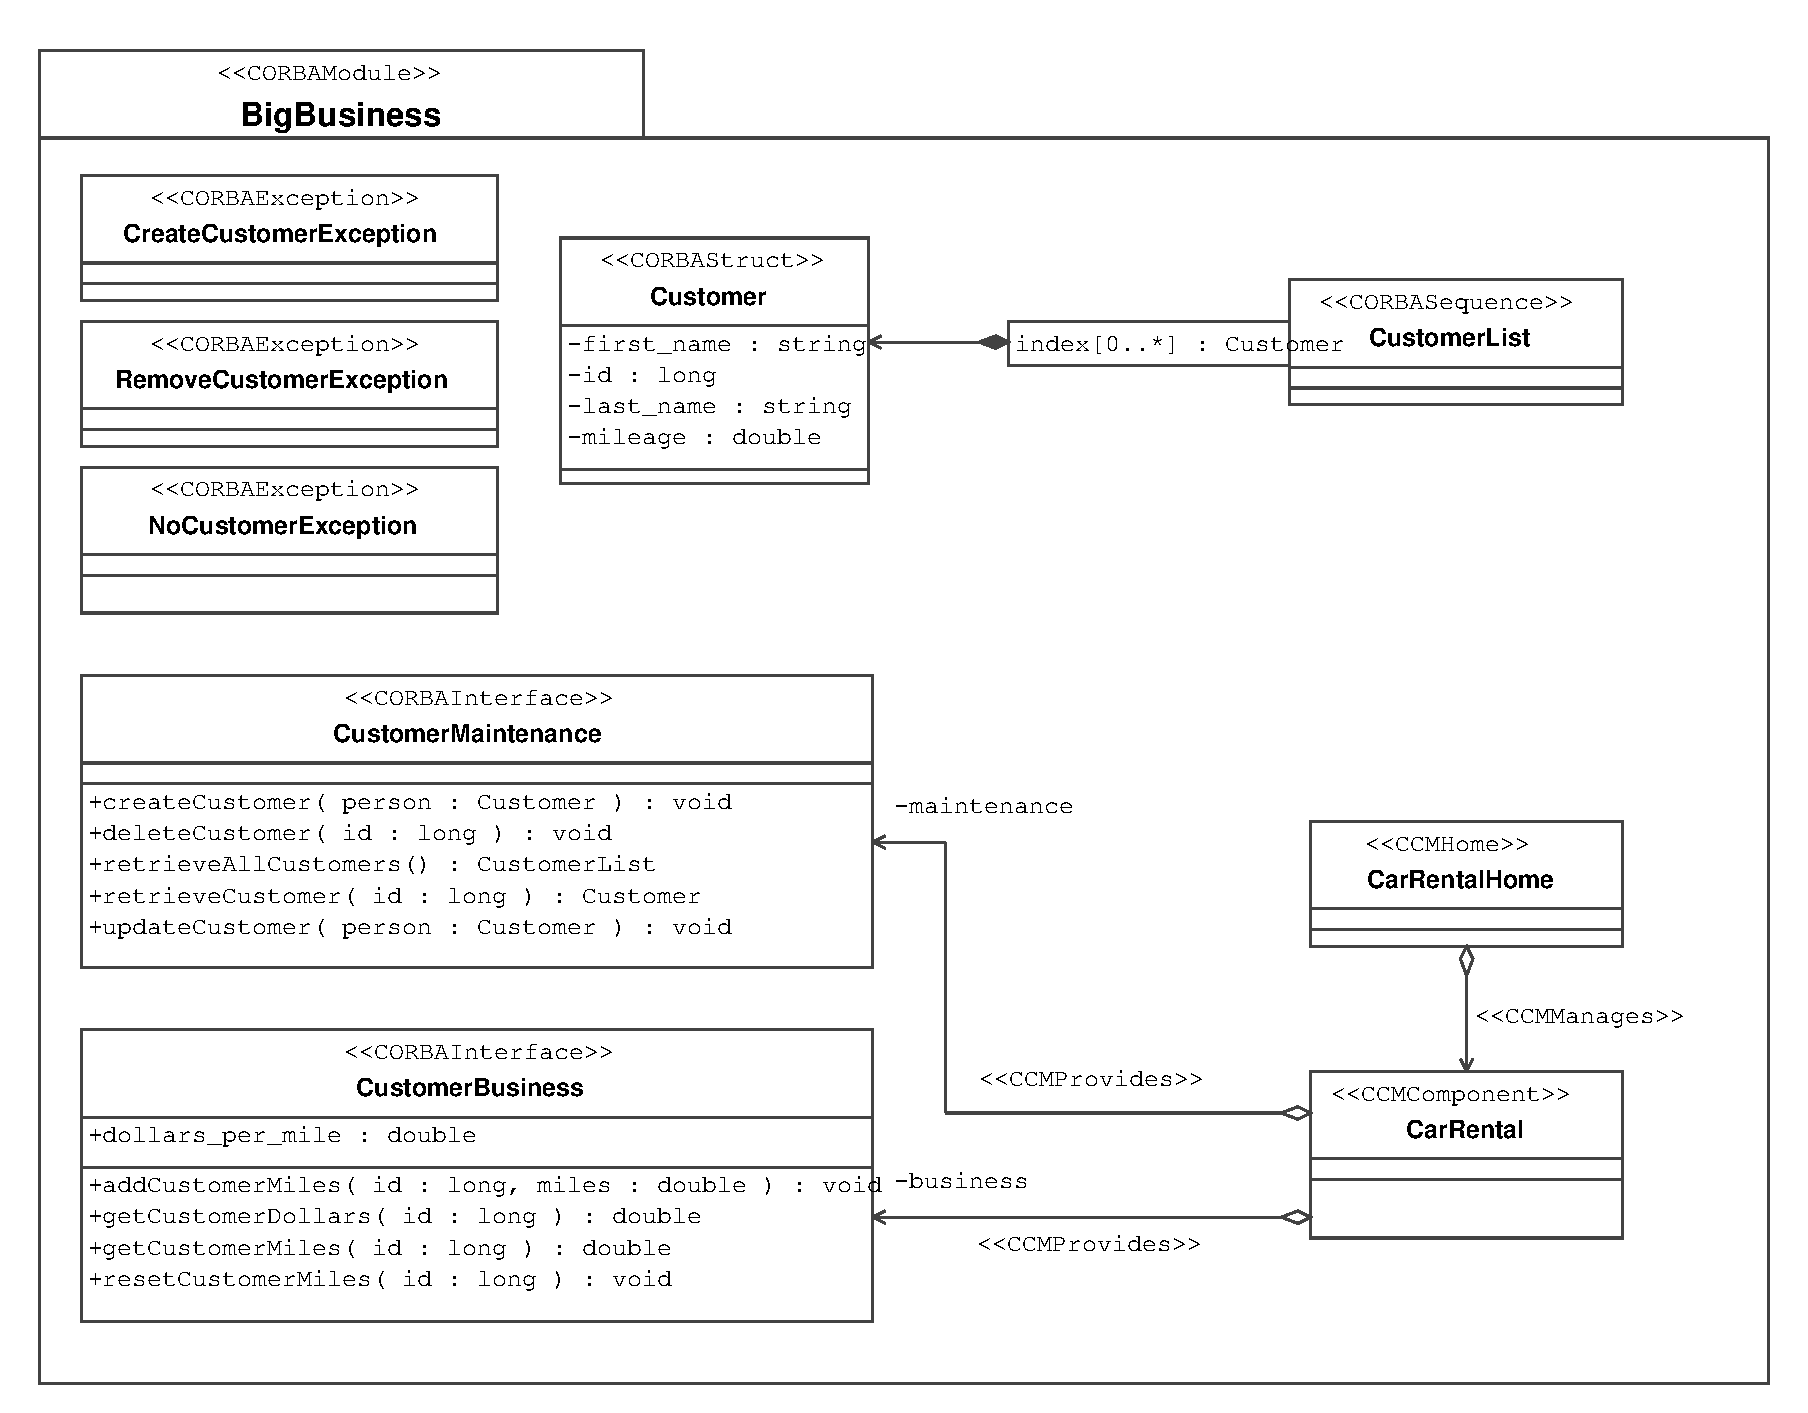
\includegraphics [width=13cm,angle=0] {uml/Example1}
        \caption{CarRental component in UML}
        \label{fig:uml-component-example}
    \end{center}
\end{figure}

We store the diagram (as an {\it XMI 1.1} file) in a directory called 
{\tt example2}, change to that directory and run the {\tt uml2idl} generator:
\begin{small}
\begin{verbatim}
    ~/example2> uml2idl uml/Example2.xml.zip example2
\end{verbatim}
\end{small}
After running {\tt uml2idl}, the new directory contains the following files:
\begin{small}
\begin{verbatim}
    example2/
    |-- example2.idl
    |-- example2.ocl
    `-- uml
        `-- Example2.xml.zip
\end{verbatim}
\end{small}

\newpage
\begin{itemize}
\item {\tt Example2.xml.zip}\\
This is the XMI file written from a UML tool.

\item {\tt example2.idl}\\ 
This file contains all generated IDL statements. 

\item {\tt example2.ocl} \\
In this file, all OCL expressions defined in the source model are stored.
Currently, we don't care about this file but we will use it in context of
Design by Contract. 
\end{itemize}

From the single IDL3 file, we generate a bunch of well structured 
IDL3 files as done with manually written files:
\begin{small}
\begin{verbatim}
    ~/example2> ccmtools-generate idl3 -o CarRental/idl3 *.idl
\end{verbatim}
\end{small}

Again, we have separated interfaces from component definitions:
\begin{small}
\begin{verbatim}
CarRental
`-- idl3
    |-- component
    |   `-- BigBusiness
    |       |-- CarRental.idl
    |       |-- CarRentalHome.idl
    |       |-- CarRentalHome_mirror.idl
    |       `-- CarRental_mirror.idl
    `-- interface
        `-- BigBusiness
            |-- CreateCustomerException.idl
            |-- Customer.idl
            |-- CustomerBusiness.idl
            |-- CustomerList.idl
            |-- CustomerMaintenance.idl
            |-- NoCustomerException.idl
            `-- RemoveCustomerException.idl
\end{verbatim}
\end{small}

That's it, we have made the first step toward MDA! 

But remember, we have only generated a component's structural description from
a UML diagram. The generated IDL file is a pure syntax description, without 
any semantics.  


%------------------------------------------------------------------------------
\section{The developers's job}
%------------------------------------------------------------------------------

It's important to know, that a developer's job does not change whether a 
component is designed in UML or IDL.
In both cases, a developer starts from the IDL3 file structure as shown above.

% $Id$
%==============================================================================
\chapter{System Development}
%==============================================================================
\begin{flushright}
{\it }
\end{flushright}

blah \dots

\newpage
% $Id$ 
%==============================================================================
\section{Nested Component Composition}
\label{NestedComponentComposition}
%==============================================================================


\begin{figure}[htb]
    \begin{center}
    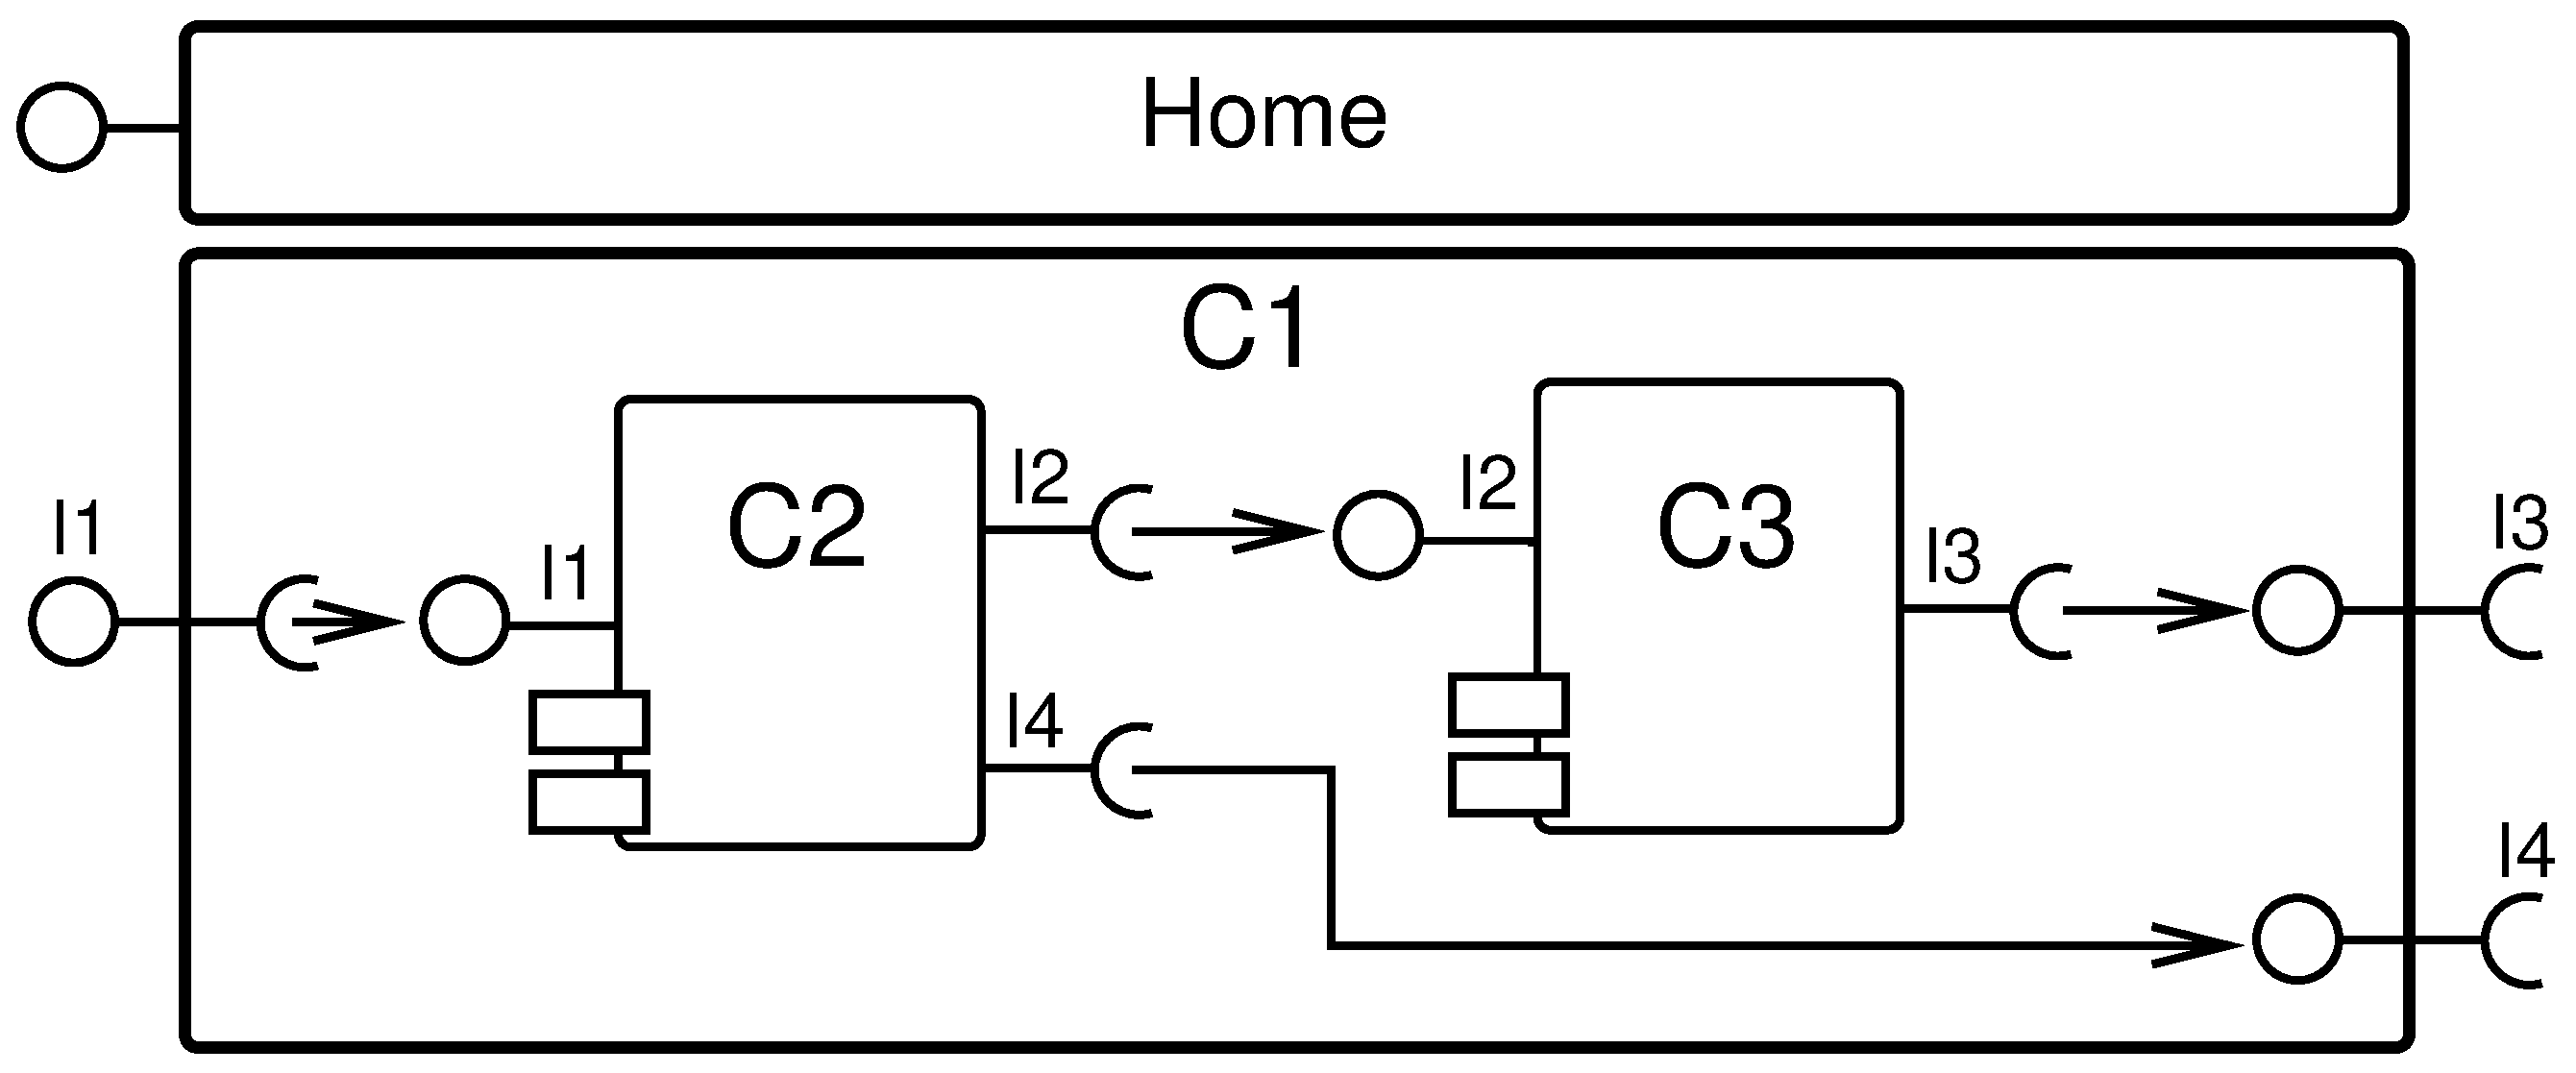
\includegraphics [width=7cm,angle=0] {ComponentModel/figures/NestedAssembly}
    \caption{ $C_{Ref}$ super component example.}
    \label{NestedAssembly}
    \end{center}
\end{figure}

Using the session facade pattern \cite{J2EECorePatterns}, 
we are able reduce a nested component composition into a flat component 
assembly that can be described by a simple CAD file.
While the inner components $C2$, $C3$ keep unchanged, the outer component $C1$ 
must be transformed into a special LwCCM component - the facade component, 
as shown in Fig.~\ref{NestedToFlatAssembly}.

\begin{figure}[htb]
    \begin{center}
    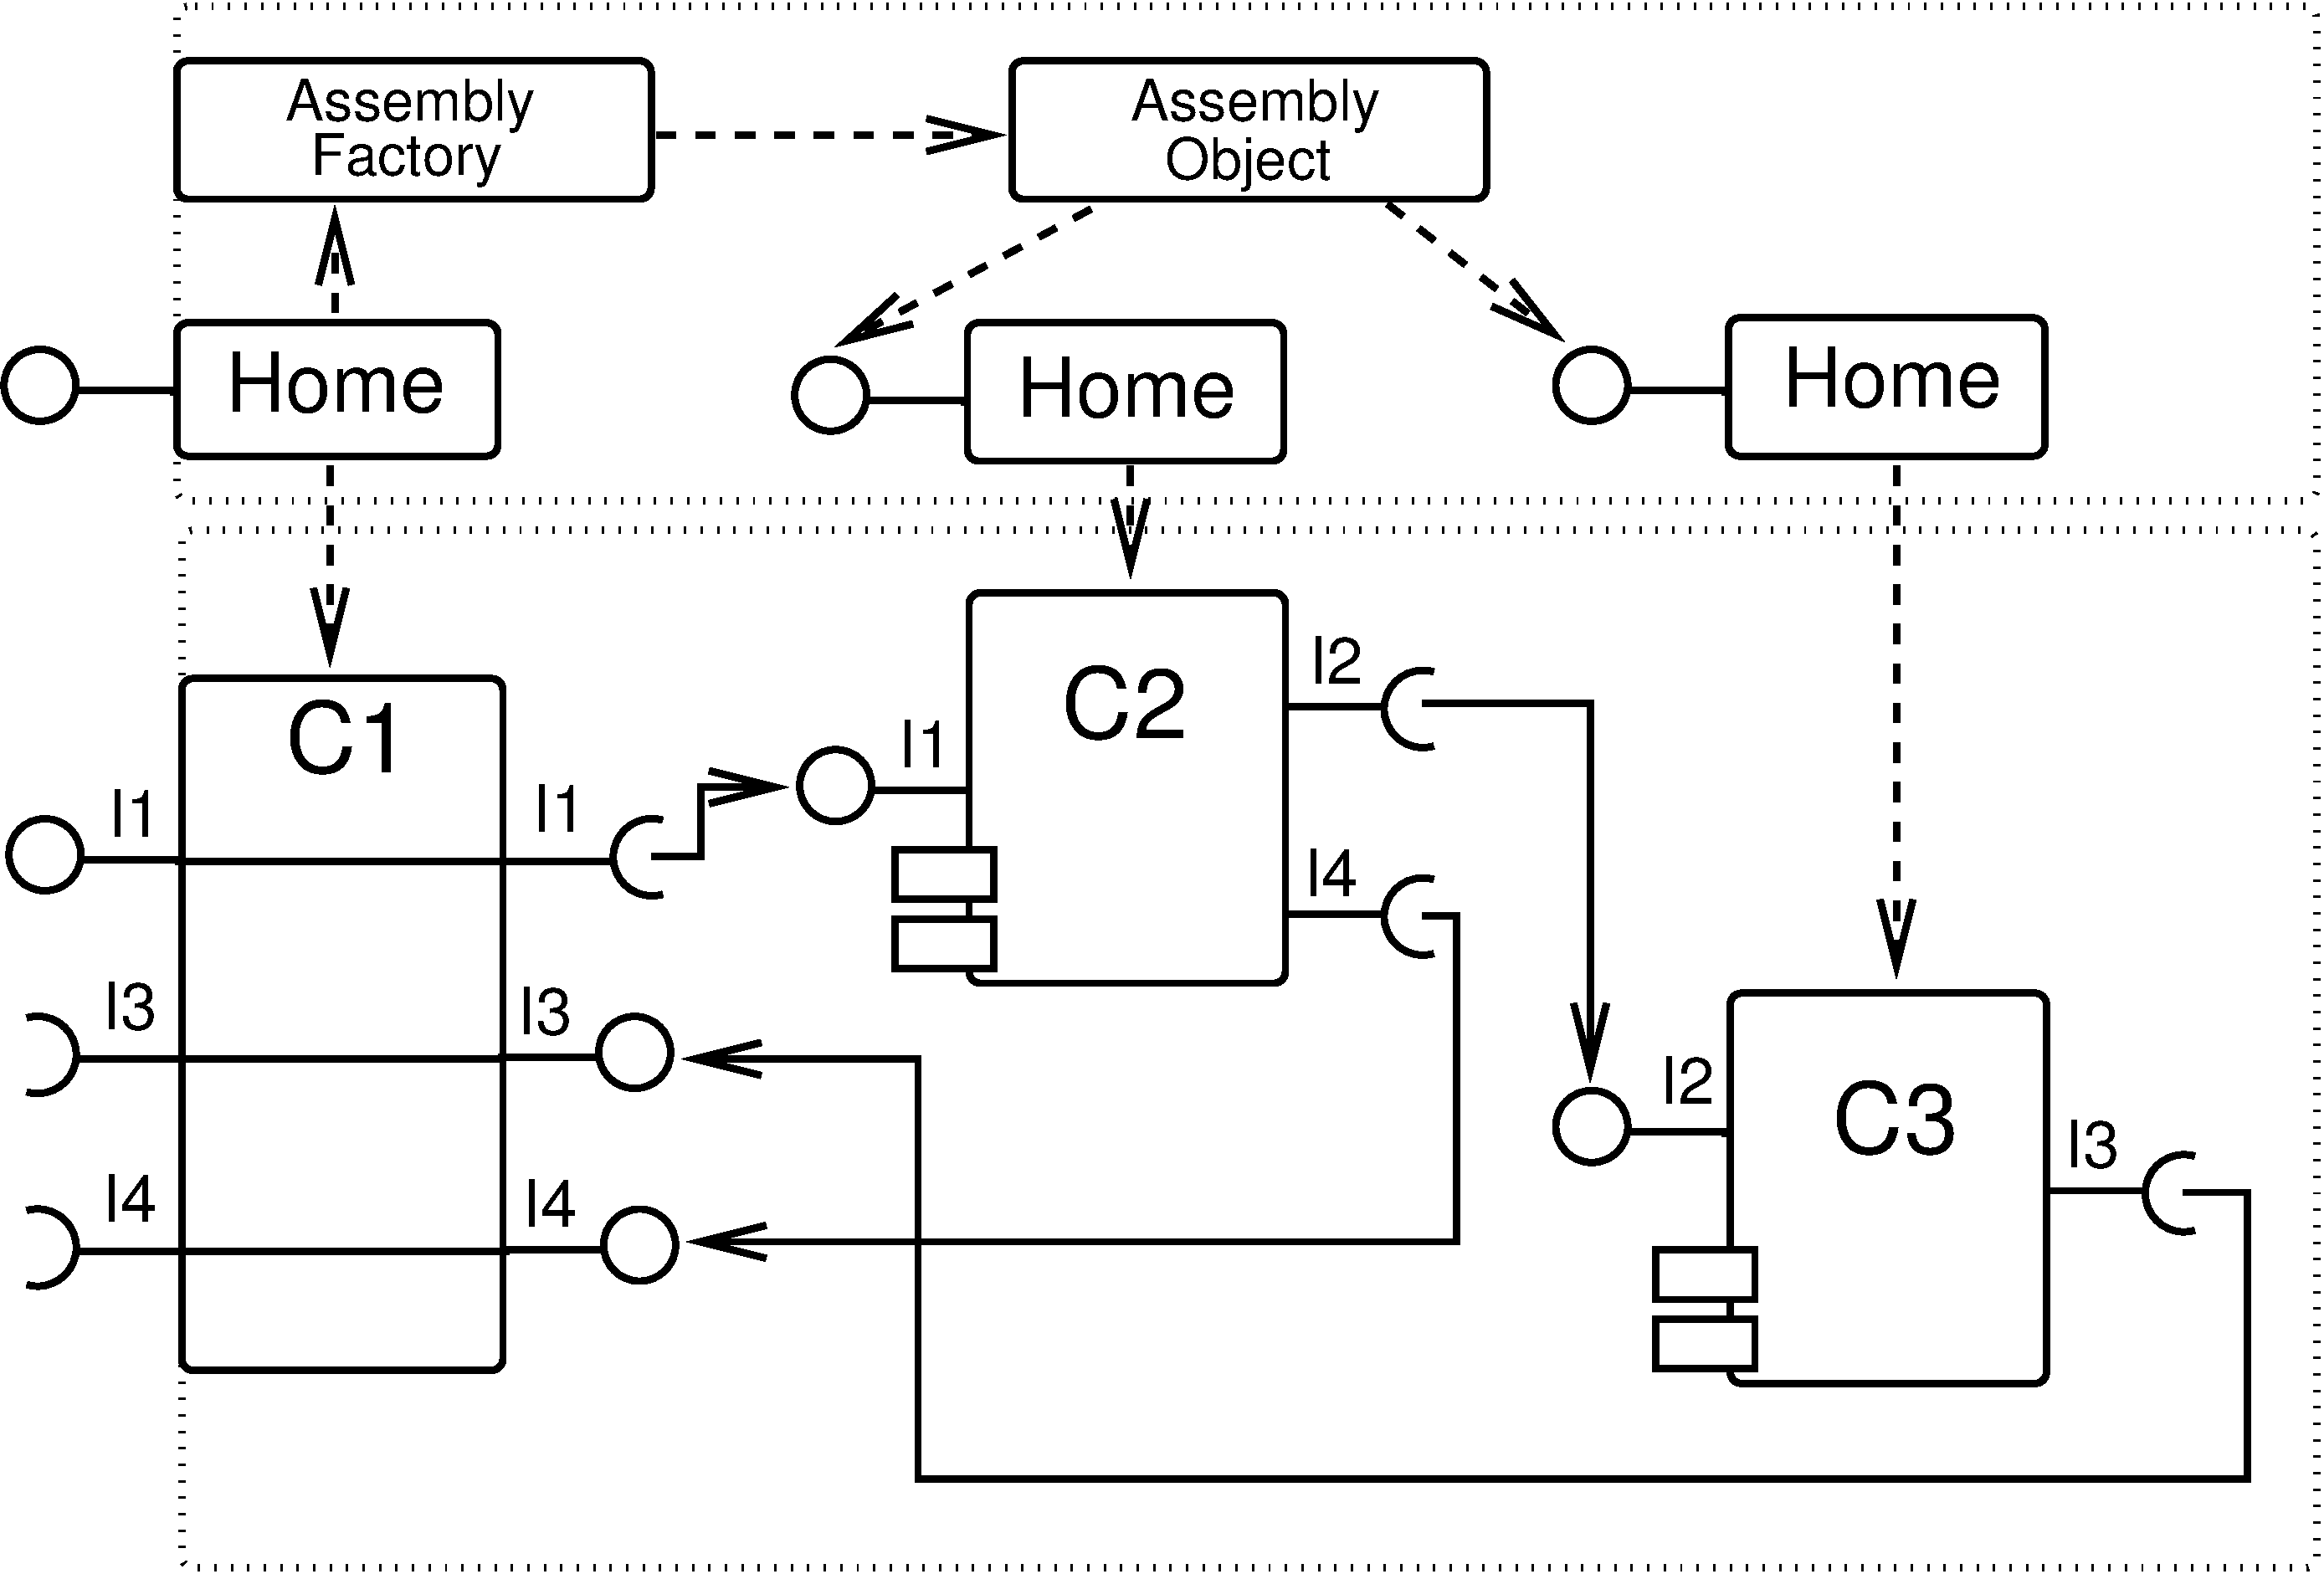
\includegraphics [width=7cm,angle=0] {ComponentModel/figures/NestedToFlatAssembly}
    \caption{Using the session facade pattern, a nested component composition
    can be reduced to a flat assembly as defined in LwCCM.}
    \label{NestedToFlatAssembly}
    \end{center}
\end{figure}

\noindent
The LwCCM facade component provides two complementary kinds of ports for each 
port defined in $C1$:
\begin{itemize}
\item {\bf Public ports.} A public port is visible to component clients and
can be accessed as a regular LwCCM component port.
 
\item {\bf Private ports.} A private port is a LwCCM port that is
not visible to component clients.
Private ports are used to connect the facade component with their inner 
component instances.
Technically, private ports are implemented like public ports, but after the
configuration phase, private ports can not be accessed by component clients. 
\end{itemize}
 
\noindent
All information about components and their connections within a super 
component are represented by an {\it Assembly Object}.
Such an assembly object is assigned to a facade component instance, and 
can be seen as a part of the facade component itself. 

For each facade component instance, an instance of the corresponding assembly
object must be created. 
To give a facade component's home the ability to create assembly object 
instances, an {\it Assembly Object Factory} must be assigned to a facade 
component home during component deployment.
With this approach, we can use regular LwCCM components and assemblies
to realize the nested component concept.

The implementation of a facade component's business logic is straightforward, 
each call to a facet method delegates to the corresponding receptacle and 
vice versa.

\vspace{3mm}
\noindent
To give a client the illusion of a single component, a facade component has to
handle some tasks behind the scenes. These are defined by the following 
sequence diagrams. 

\begin{figure}[htb]
    \begin{center}
    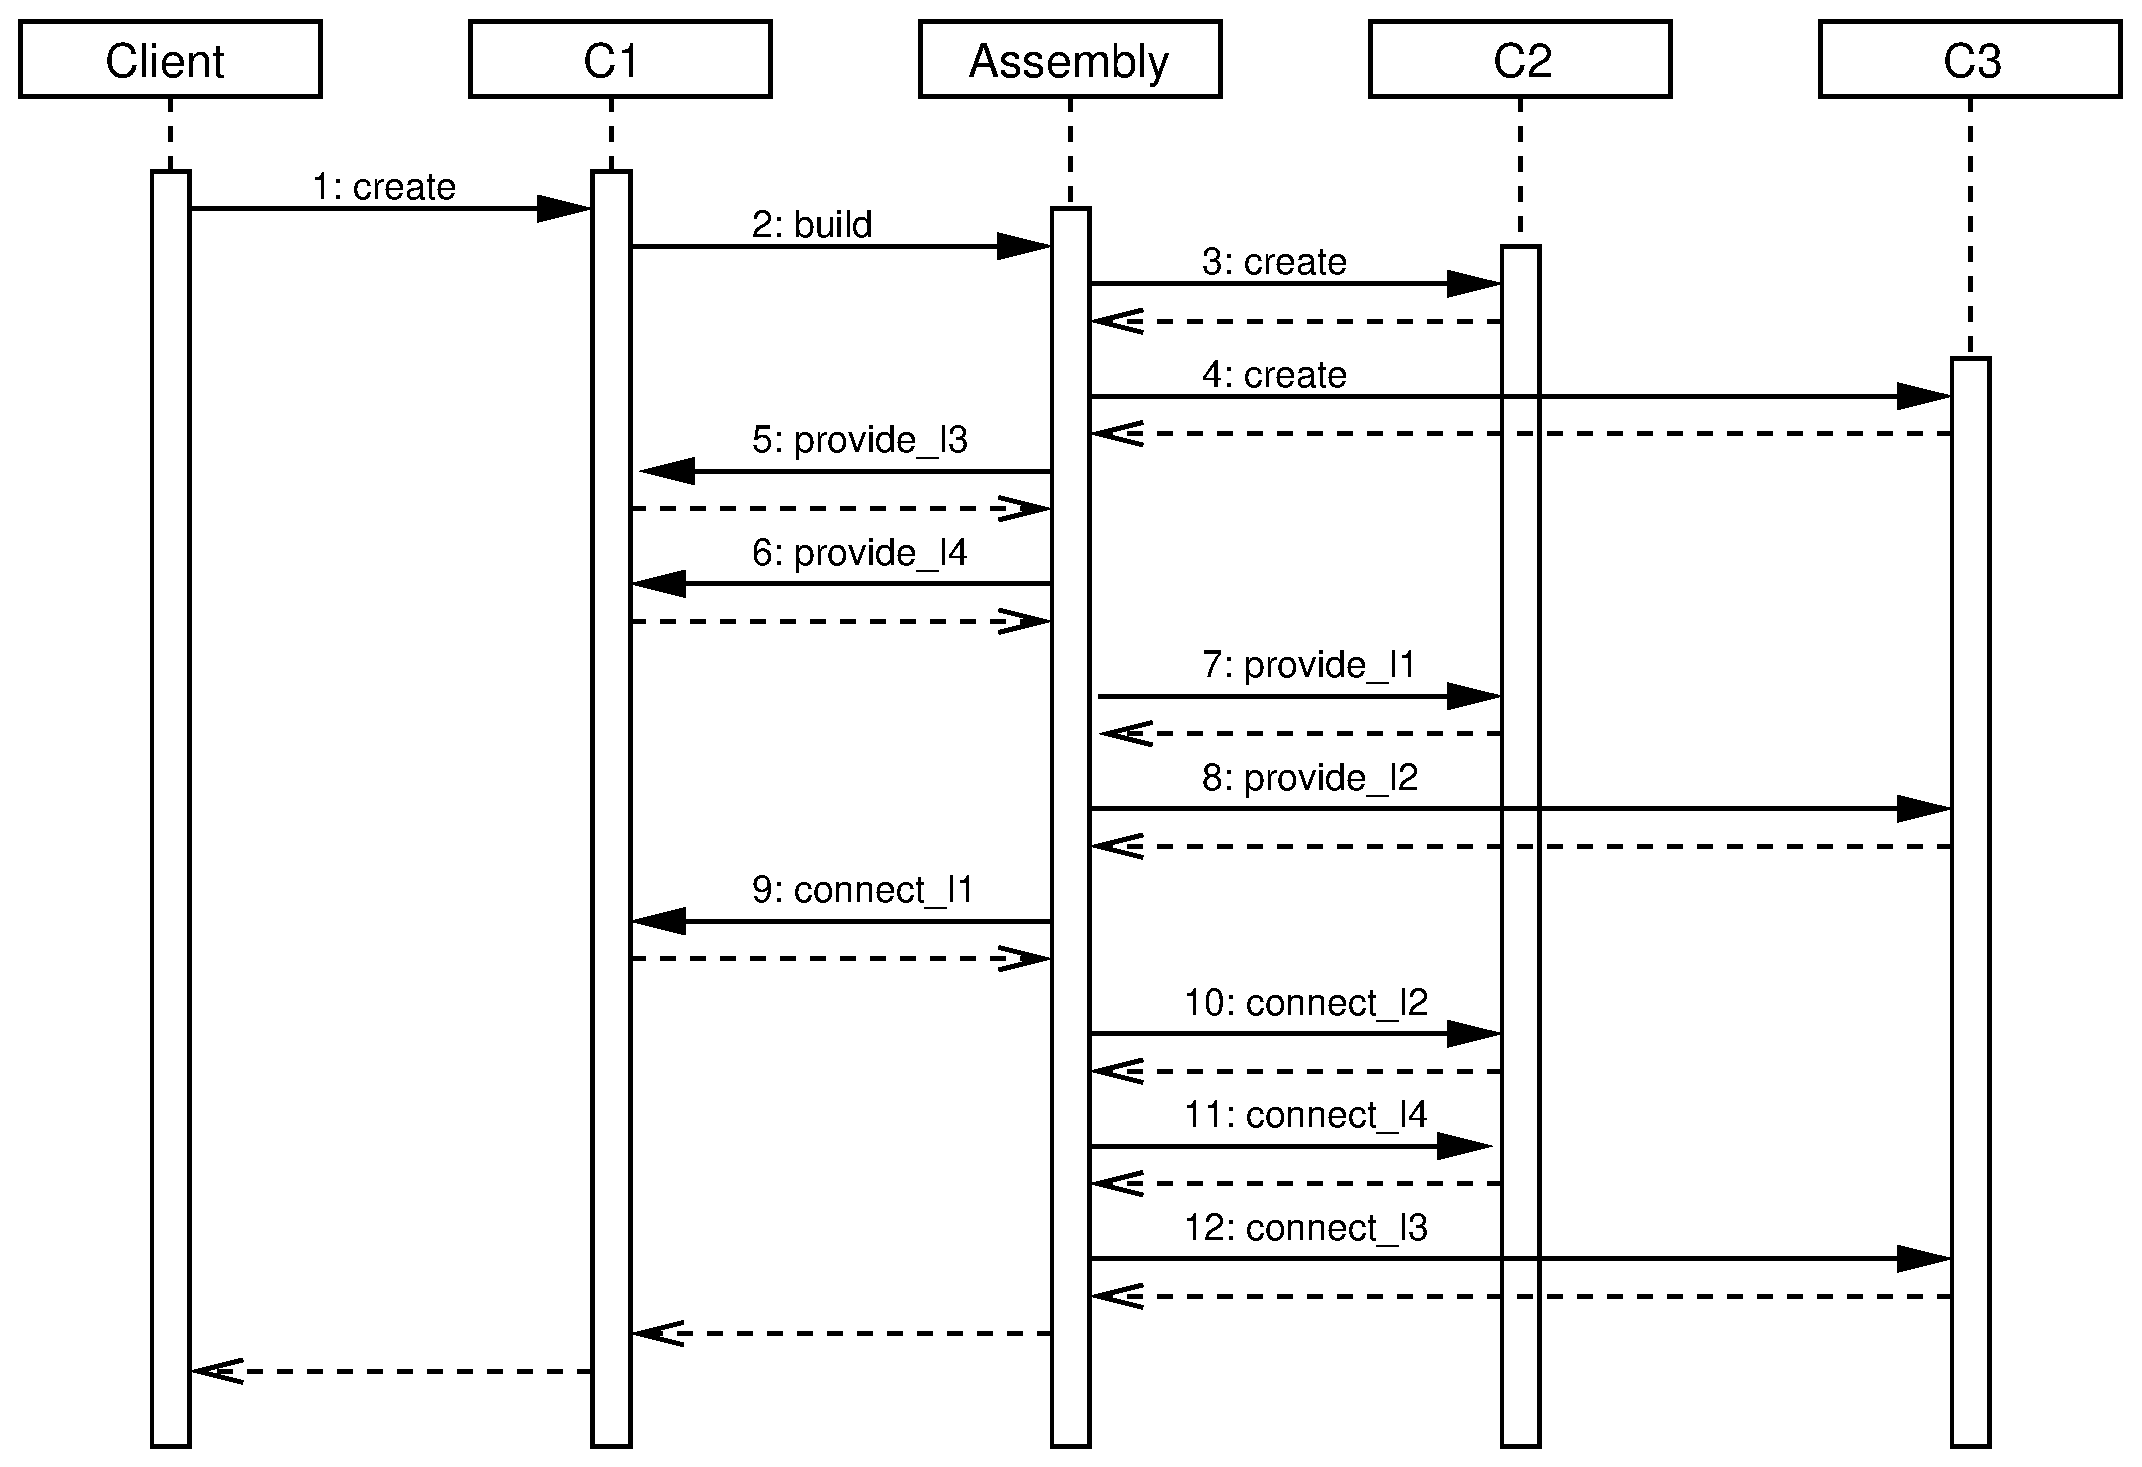
\includegraphics [width=12cm,angle=0] {ComponentModel/figures/SuperComponentCreate}
    \caption{Create a super component of Fig~\ref{NestedToFlatAssembly}.}
    \label{SuperComponentCreate}
    \end{center}
\end{figure}

\noindent
From a client's point of view, there is only one component $C_1$ that can be
instantiated by $C_1$'s home (Fig.~\ref{SuperComponentCreate}).
In fact, $C_1$ calls the {\tt build} method of the associated assembly object.
This assembly object in turn instantiates $C_2$ and $C_3$ and establishes all 
defined connections between these component instances.
After these activities, the assembly object returns to $C_1$ that finishes 
its create method.

Of course, $C_1$ itself can be part of another super component or connected 
to other components as well.
LwCCM defines the end of a component's configuration phase by calling the
{\tt configuration\_complete} method on each component instance.
In the case of a super component, this call must be delegated to all 
subcomponent instances (Fig.~\ref{SuperComponentConfigurationComplete}).
Before $C_1$ can return from {\tt configuration\_complete}, it has to lock all
private ports to prevent clients from directly accessing contained component 
instances.

\begin{figure}[htb]
    \begin{center}
    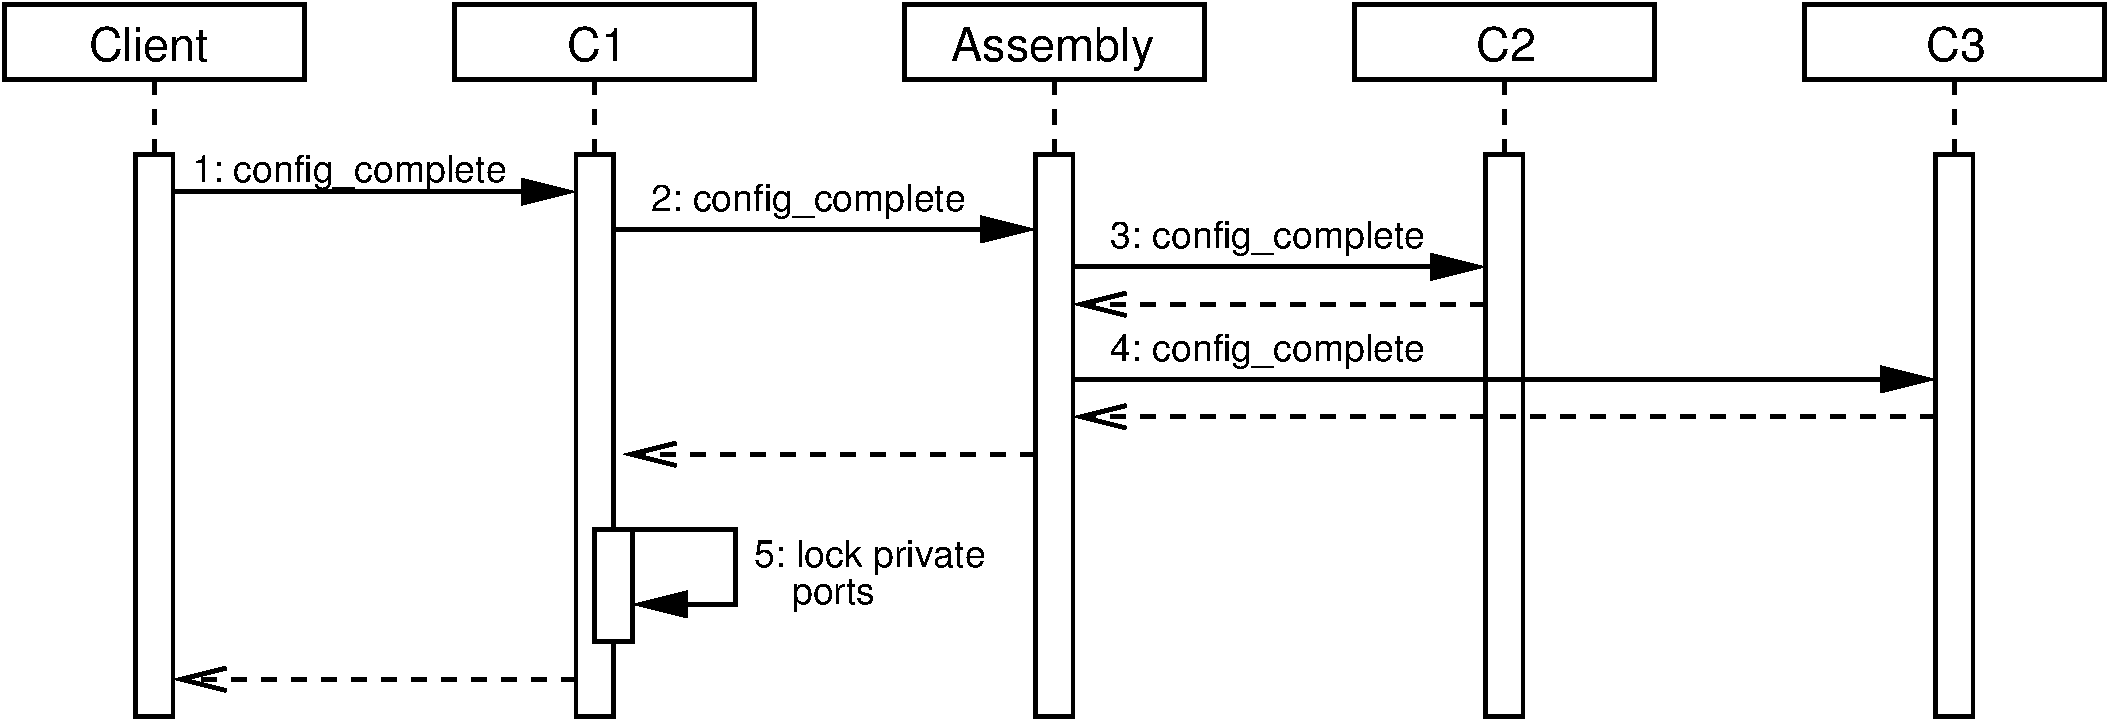
\includegraphics [width=12cm,angle=0] 
		     {ComponentModel/figures/SuperComponentConfigurationComplete}
    \caption{Completion of super component configuration phase.}
    \label{SuperComponentConfigurationComplete}
    \end{center}
\end{figure}

\noindent
Fig.~\ref{SuperComponentRemove} shows how a super component instance is removed:
$C_1$ triggers the assembly object to disconnect and destroy
all contained component instances.

\begin{figure}[htb]
    \begin{center}
    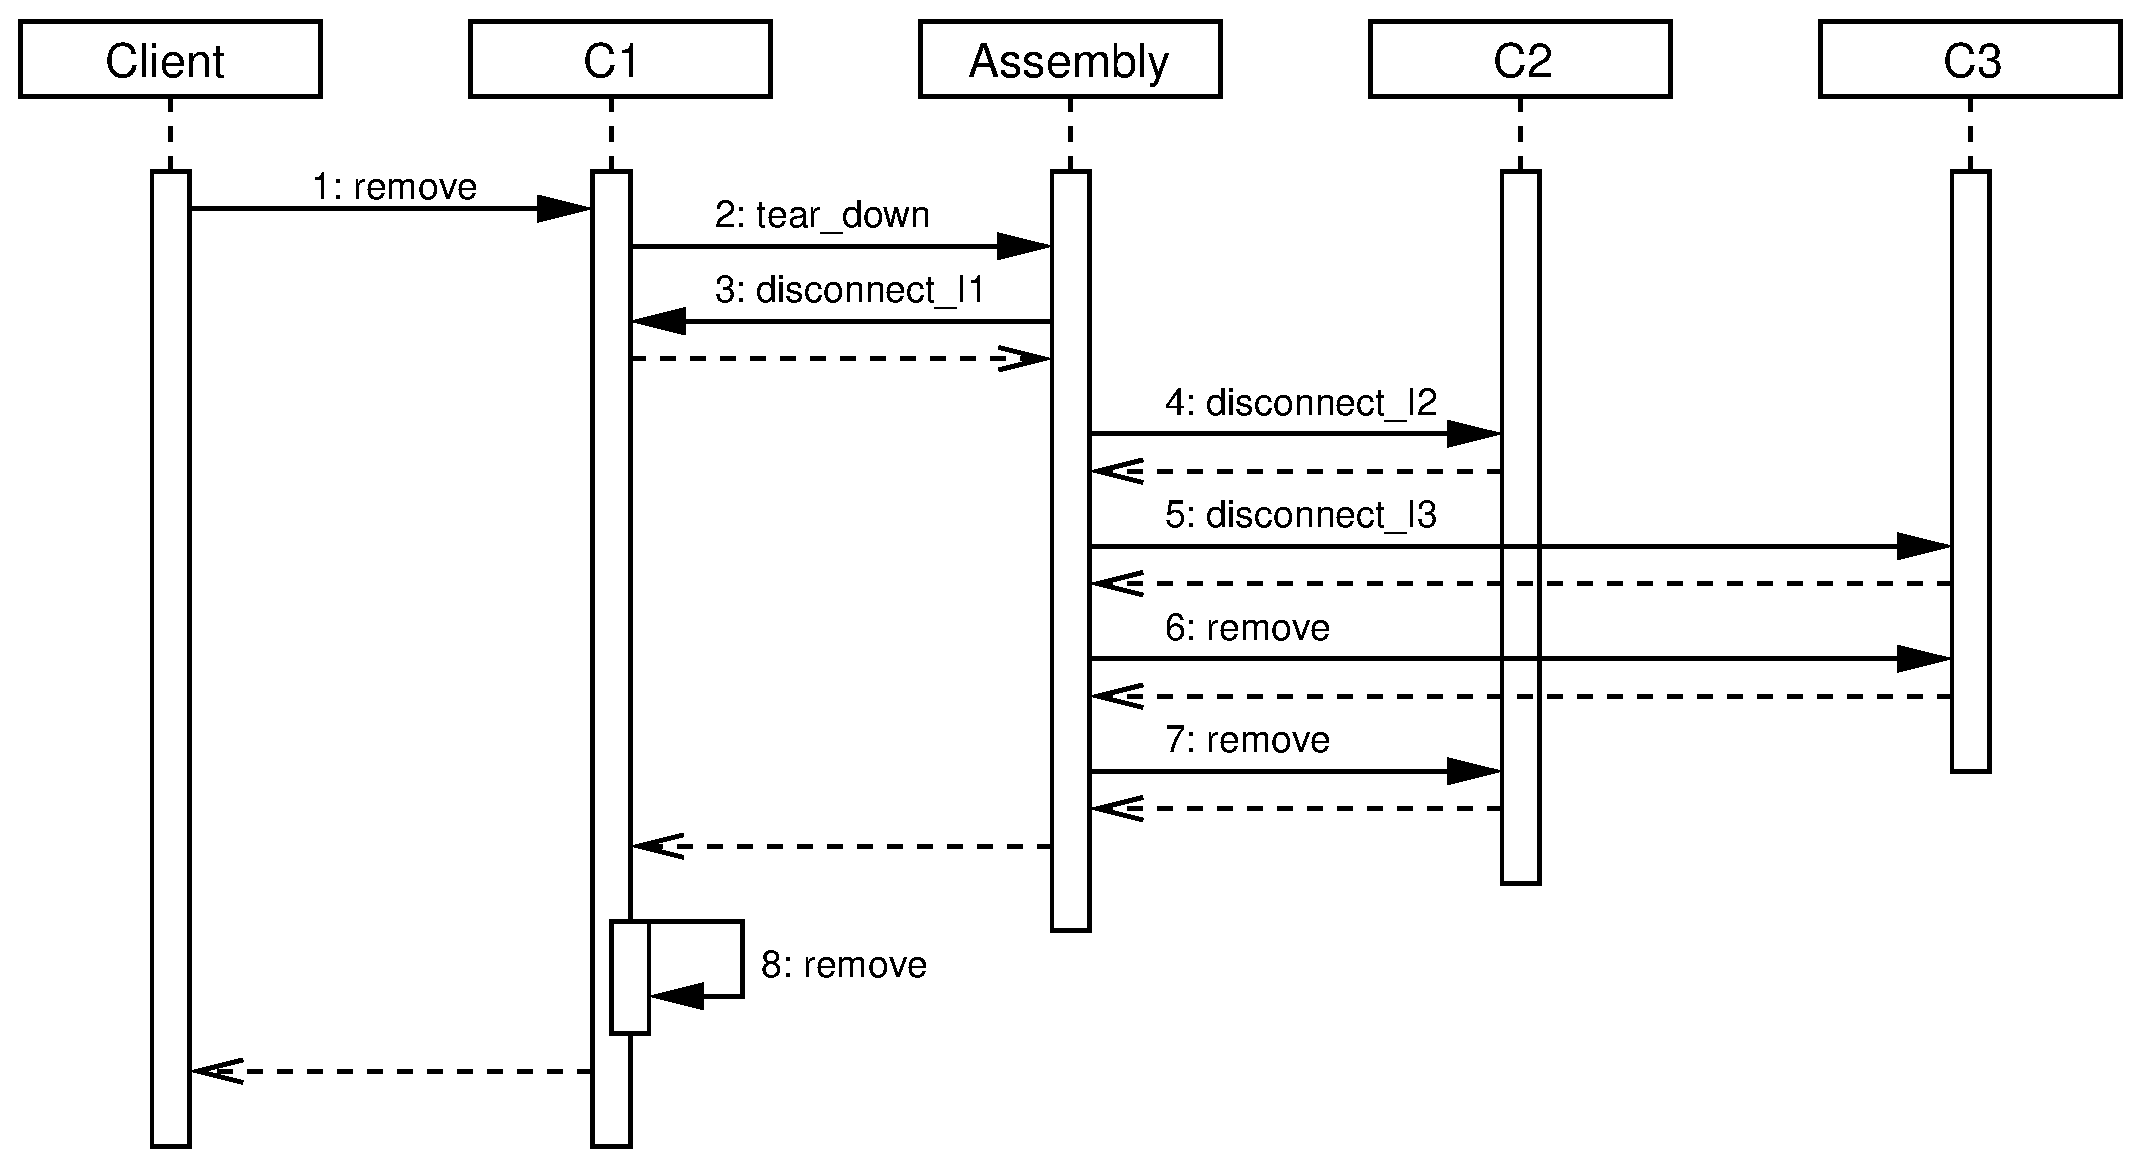
\includegraphics [width=12cm,angle=0] {ComponentModel/figures/SuperComponentRemove}
    \caption{Removal of a super component.}
    \label{SuperComponentRemove}
    \end{center}
\end{figure}

\noindent
A component client can handle
the super component in the same way as a regular LwCCM component.
Also, a simple LwCCM component can be seen as a special case of a super
component with an empty assembly.
Thus, both components and assemblies has been reduced to a single concept.



% Assemblies of components

% ModelDrivenSystemdevelopment

%% $Id$
%==============================================================================
\chapter{System Deployment}
%==============================================================================
\begin{flushright}
{\it }
\end{flushright}



\newpage
% $Id$

%==============================================================================
\section{Remote Component Structure}
%==============================================================================

While we have implemented a local version of CORBA Components, 
the LwCCM specification defines remote components only.
Remote components are built up from CORBA objects that implement defined
IDL interfaces.
Because of the specified mapping from IDL3 to IDL2, the generated IDL2 files 
can be processed by every existing IDL compiler. In addition to CORBA stubs
and skeletons, remote component logic as well as CORBA component containers
must be implemented too. 
To be compliant to the LwCCM specification, we have developed a way to
adapt local components into remote LwCCM components - the 
{\bf Local Component Adapter Concept} (LCAC).

LCAC allows to add remote communication
for each port transparently for business logic.
Fig.~\ref{LcacOverview} shows how a given local component implementation
can be extended to a remote LwCCM component.

\begin{figure}[htbp]
    \begin{center}
    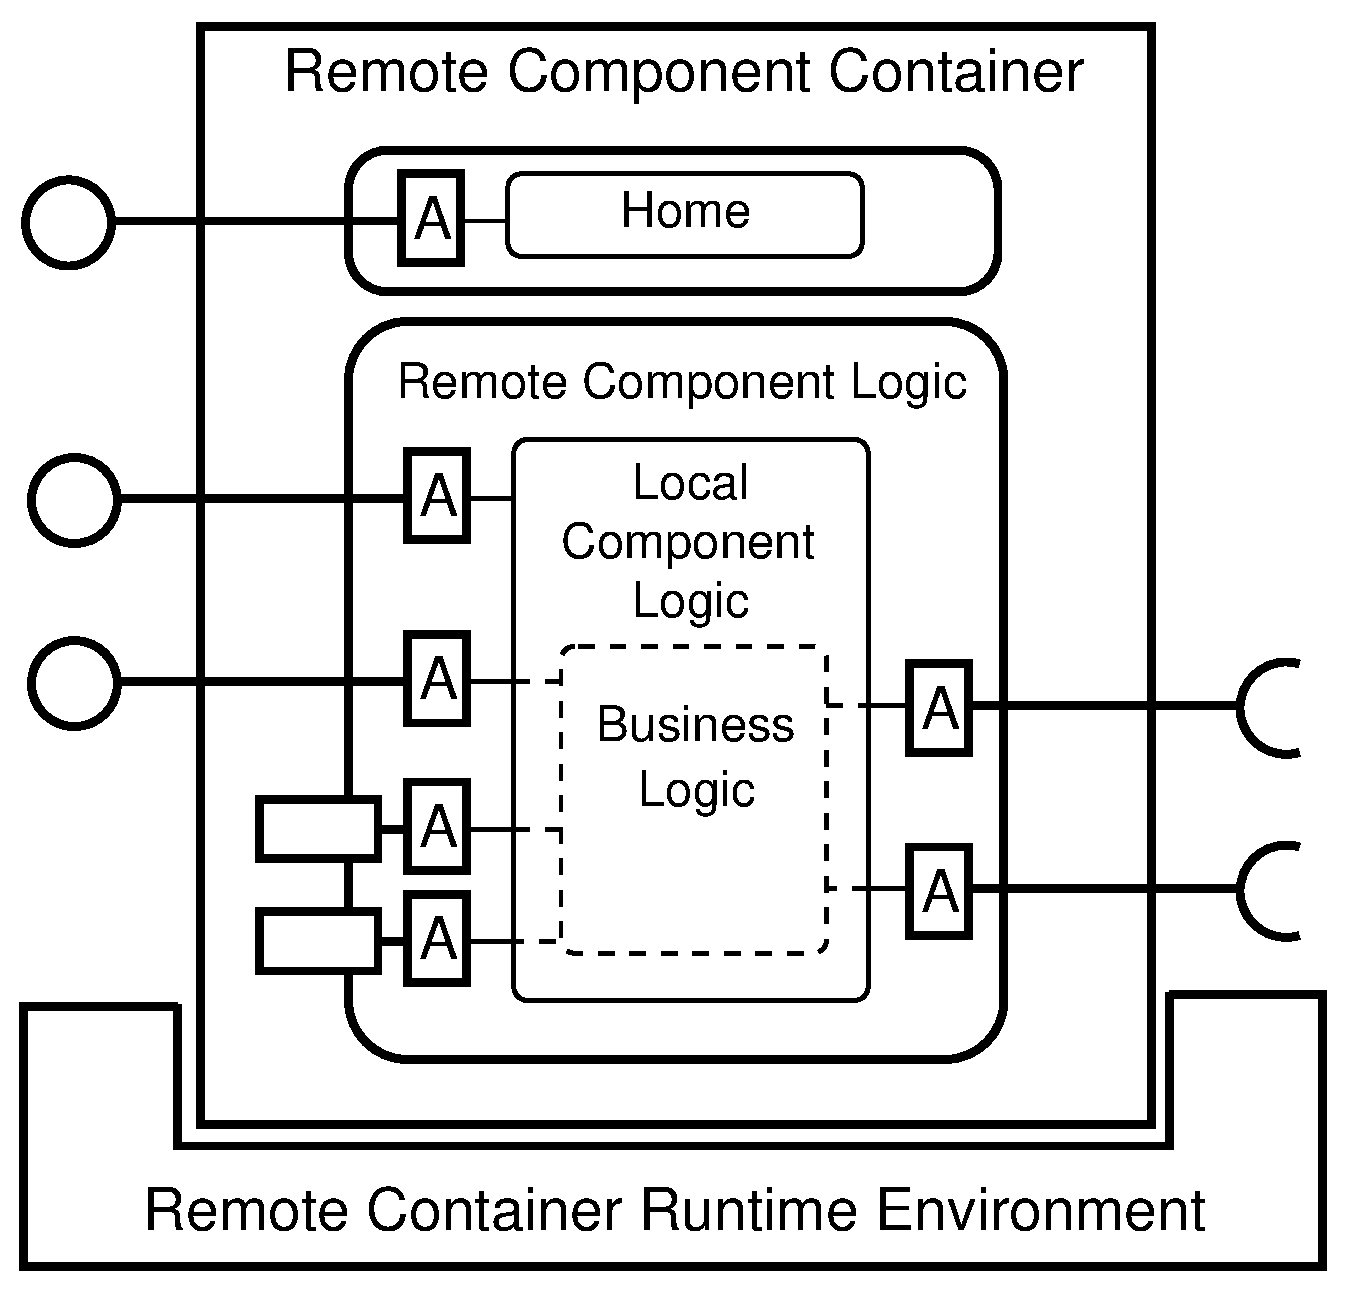
\includegraphics [width=5.5cm,angle=0] {figures/LocalAdapterConcept.eps}
    \caption{A local component can be embedded in a remote component logic
    that will be managed by a remote component container.}
    \label{LcacOverview}            
    \end{center}
\end{figure}

\noindent
The point is that we can use local components without changing them.
Thus, for a remote accessible component that provides at least one remote 
port, some additional code will be involved.

\begin{description}
\item [Remote component logic.]
A glue code layer is responsible for embedding a local component into a 
remote CORBA component. 
This remote component logic hosts a local component.
That means, its local component logic and business logic.  
Such a structure ensures that local ports can be used side by side to remote
ports.

\item [Adapter set.]
For a given IDL interface that defines a component port's syntax, a local and 
a remote implementation is generated. 
Using a set of adapter classes, these two worlds can fit together transparently.
In addition to component ports, adapters must be provided for component homes
as well as the component's equivalent interface.

\item [Remote component container.]
For each remote component type, a generic component container is used to
manage CORBA component instances.
In contrast to a local component container that can have a simple structure, a
remote container is also responsible for sophisticated {\it Quality of Service} 
(QoS) tasks.

\item [Remote container runtime environment.]
With increasing QoS functionality, the requirements to a remote container
runtime environment are growing too.
Besides an {\it Object Request Broker} (ORB), that handles CORBA requests,
libraries for multi--threading and process management implementation must 
be available.  
\end{description}

\noindent
This adapter concept is a powerful tool especially in heterogeneous 
environments. Besides the choice between local and remote connections, 
a deployment process can also decide to use different middleware technologies.


The fact that a local component is wrapped by a remote component becomes 
obvious from Fig.~\ref{StructureOfRemoteComponents}. All classes of a local
component remain unchanged, while some new ``remote'' classes have been added.

\begin{figure}[htbp]
    \begin{center}
    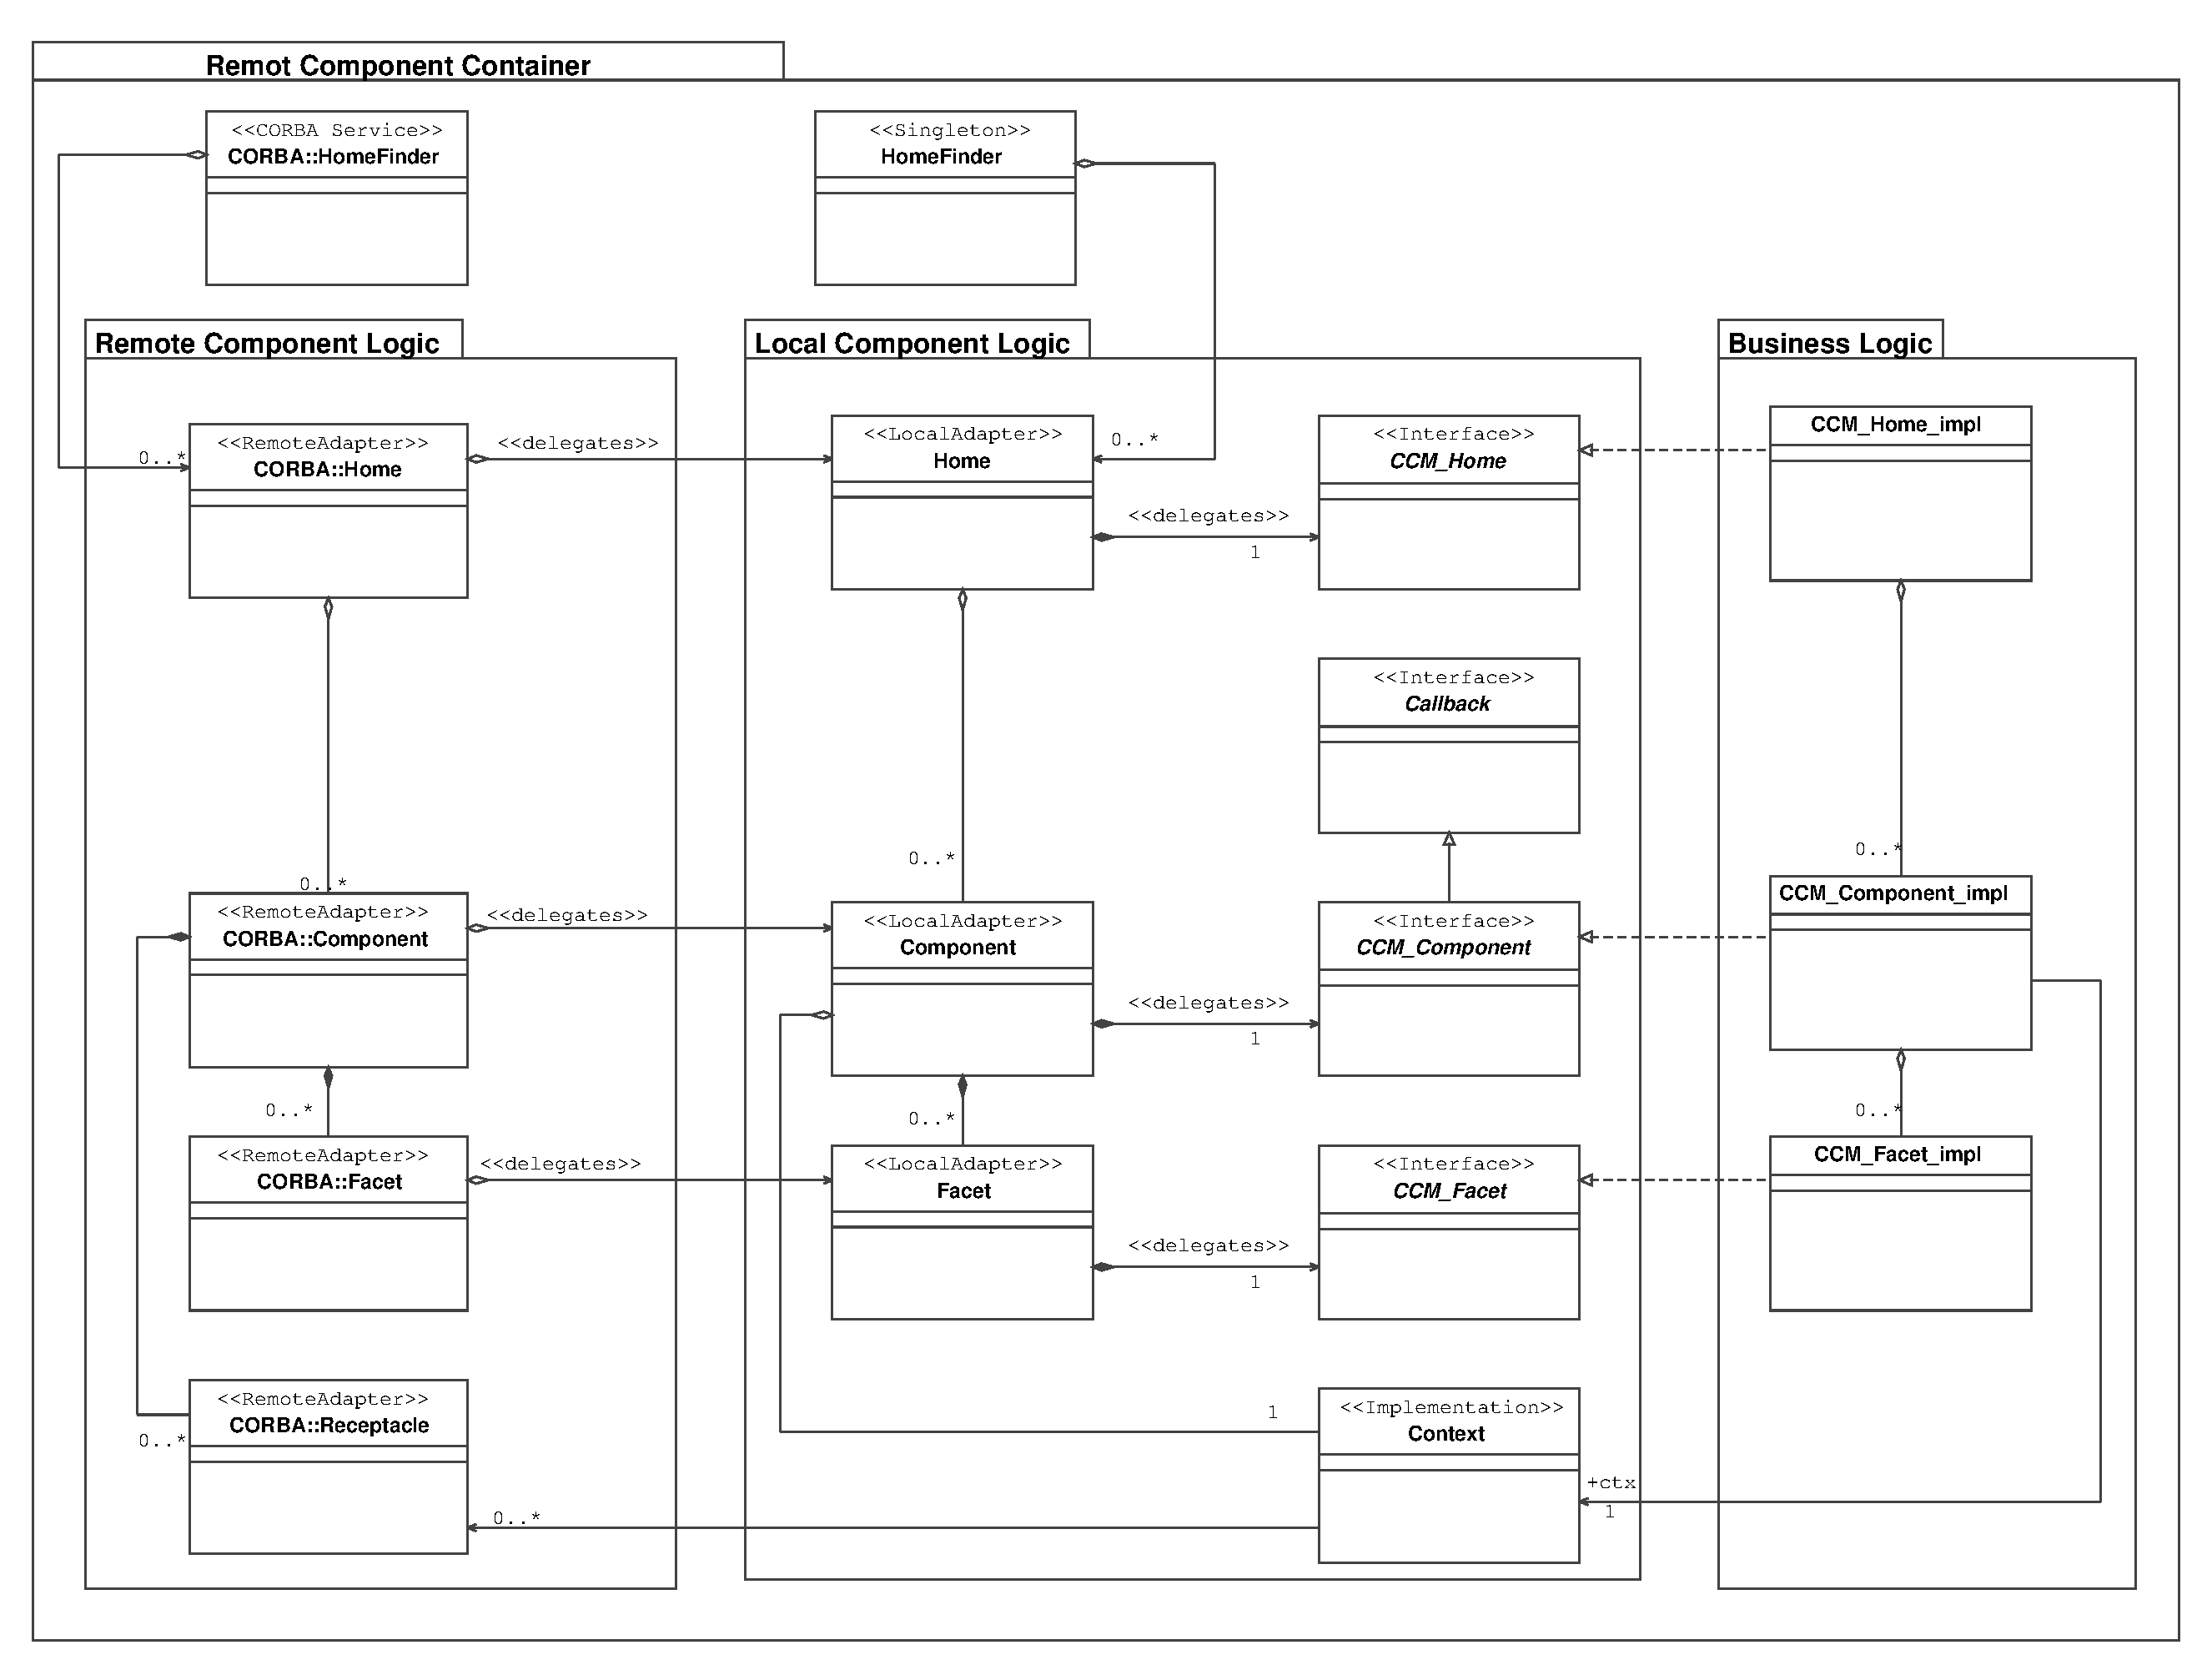
\includegraphics [width=15cm,angle=0] 
		     {uml/StructureOfRemoteComponents.eps}
    \caption{Simplified structure of a remote component implementation,
    showing the relationship between corresponding local and remote components.}
    \label{StructureOfRemoteComponents}            
    \end{center}
\end{figure}

\noindent
The remote structure is very similar to a local component's structure 
(Fig.~\ref{StructureOfLocalComponents}), thus, we can compare interactions
between a local and a remote component with interactions between business logic
and local component logic:

\begin{description}
\item [Calling component methods.]
A remote client calls methods on a remote adapter that delegates this
calls to a local component which uses a local adapter to delegate these calls
to business logic.
In each adapter, pre- and a post-invoke processing can take place 
(Fig.~\ref{RemoteComponentCall}).
\begin{figure}[htbp]
    \begin{center}
    \includegraphics [width=9cm,angle=0] 
		     {figures/RemoteComponentCall.eps}
    \caption{A remote call of a component's method is delegated twice
    allowing pre- and post-invoke processing.}
    \label{RemoteComponentCall}            
    \end{center}
\end{figure}

These two indirection layers allow non--functional extensions to 
components without changes in business logic. 
This separation of concerns is a cornerstone in component
based development.

\item [Invoking callback methods.]
Callback methods implemented by business logic can be
triggered either from local or remote component logic and their corresponding
container implementations to control a component's life cycle.

\item [Using context methods.]
Component business logic uses the {\tt Context} object to access container
functionality as well as component receptacles.
In the case of remote components, receptacles can be either local or remote
ports. Both kinds of receptacles can be accessed via local context
object methods. While local receptacles are connected directly to local facets,
remote receptacles are intercepted by a receptacle adapter.
\end{description}

\noindent
Based on LCAC, an existing LwCCM container implementation could be used to host 
local components, thus, we could combine an existing CORBA application server 
with the presented extensions in the context of local components. 


\newpage
% $Id$

%==============================================================================
\section{Car rental example}
%==============================================================================

We reuse our well known {\tt CarRental} component
to show how a local component can be extended to a CORBA component.
The local {\tt CarRental} component is organized in the following file 
structure:

\begin{small}
\begin{verbatim}
   server
   |-- component
   |   `-- CarRental
   |       |-- CCM_BigBusiness_ccm_local_component_CarRental
   |       `-- CCM_BigBusiness_ccm_local_component_CarRental_share
   |-- idl3
   |   |-- component
   |   |   `-- BigBusiness
   |   `-- interface
   |       `-- BigBusiness
   `-- interface
       |-- CCM_BigBusiness_ccm_local
       `-- CCM_BigBusiness_ccm_local_adapter
\end{verbatim}
\end{small}


%------------------------------------------------------------------------------
\subsubsection{Generate CORBA component adapters}
%------------------------------------------------------------------------------

For a remote CORBA component all IDL3 files must be mapped to equivalent
IDL2 files, as defined in the CCM specification \cite{CCMSpecification}.
Using the CCM Tools, this mapping can be done with a single call: 
\begin{small}
\begin{verbatim}
> ccmtools idl2 -o server/component/CarRental/CCM_corba_stubs \ 
                -Iserver/idl3/interface \
                -Iserver/idl3/component \
                server/idl3/interface/BigBusiness/*.idl \
                server/idl3/component/BigBusiness/CarRental*.idl
\end{verbatim}
\end{small}

The result of this IDL3 to IDL2 mapping is a {\tt CCM\_corba\_stubs} 
subdirectory, where all IDL2 files are stored.
\begin{small}
\begin{verbatim}
server/
|-- component
|   |-- CarRental
|   |   |-- CCM_corba_stubs
|   |   |   |-- BigBusiness_CarRental.idl
|   |   |   |-- BigBusiness_CarRentalHome.idl
|   |   |   |-- BigBusiness_CreateCustomerException.idl
|   |   |   |-- BigBusiness_Customer.idl
|   |   |   |-- BigBusiness_CustomerBusiness.idl
|   |   |   |-- BigBusiness_CustomerList.idl
|   |   |   |-- BigBusiness_CustomerMaintenance.idl
|   |   |   |-- BigBusiness_NoCustomerException.idl
|   |   |   |-- BigBusiness_RemoveCustomerException.idl
|   |   |   |-- Makefile
|   |   |   |-- Makefile.py
|   |   |   `-- build.xml
\end{verbatim}
\end{small}

Additionally, the generated  {\tt CCM\_corba\_stubs/Makefile} will
trigger Mico's IDL compiler to create C++ stub and skeleton files:
\begin{small}
\begin{verbatim}
> make -C server/component/CarRental/CCM_corba_stubs
\end{verbatim}
\end{small}

Besides the CORBA stubs and skeletons, a set of adapters is used to
convert between CORBA objects and local component classes.
These component adapters are generated with the following CCM Tools call:
\begin{small}
\begin{verbatim}
> ccmtools c++remote -o server/component/CarRental \
                     -Iserver/idl3/interface \
                     -Iserver/idl3/component \
                     server/idl3/interface/BigBusiness/*.idl \
                     server/idl3/component/BigBusiness/*.idl
\end{verbatim}
\end{small}

This additional component logic is stored within the {\tt CarRental}
component directory (see {\tt CCM\_*\_ccm\_remote\_component\_*} and 
{\tt CCM\_corba\_converter} subdirectories).
\begin{small}
\begin{verbatim}
server/
|-- component
|   |-- CarRental
|   |   |-- CCM_BigBusiness_ccm_local_component_CarRental
|   |   |-- CCM_BigBusiness_ccm_local_component_CarRental_share
|   |   |-- CCM_BigBusiness_ccm_remote_component_CarRental
|   |   |-- CCM_corba_converter
|   |   |-- CCM_corba_stubs
\end{verbatim}
\end{small}

Remember, the LCAC allows to extend a local component to a CORBA component
without business logic changes. 


\newpage
%------------------------------------------------------------------------------
\subsubsection{Install the remote {\tt CarRental} component}
%------------------------------------------------------------------------------
Finally, we can run {\tt Confix} to build and install this remote component:
\begin{small}
\begin{verbatim}
> confix.py --packageroot=`pwd`/server --bootstrap --configure 
            --make --targets=install
\end{verbatim}
\end{small}

After installing this remote component, the component repository contains
the following structure for C++ header files and libraries:
\begin{small}
\begin{verbatim}
include/
|-- BigBusiness
|   `-- ccm
|       |-- local
|       |   `-- component
|       |       |-- CarRental
|       |       `-- CarRental_mirror
|       `-- remote
|           `-- component
|               `-- CarRental
\end{verbatim}
\end{small}

\begin{small}
\begin{verbatim}
lib/
|-- libCarRental_component_CarRental.a
|-- libCarRental_..._ccm_local_component_CarRental.a
|-- libCarRental_..._ccm_remote_component_CarRental.a
|-- libCarRental_component_CarRental_CCM_corba_converter.a
|-- libCarRental_component_CarRental_CCM_corba_stubs.a
|-- libCarRental_component_CarRental_mirror.a
|-- libCarRental_component_CarRental_mirror_..._CarRental_mirror.a
|-- libCarRental_interface_CCM_BigBusiness_ccm_local_adapter.a
\end{verbatim}
\end{small}


\newpage
%------------------------------------------------------------------------------
\subsubsection{Implement a CORBA component server}
%------------------------------------------------------------------------------

A remote component must be launched in its own process to handle CORBA calls
from clients or other remote components.
For that reason, we create a new directory called {\tt corba\_server}
that hosts the code for a pretty simple CORBA server.
\begin{small}
\begin{verbatim}
corba_server/
|-- Makefile.py
`-- server.cc
\end{verbatim}
\end{small}

The {\tt server.cc} code, shows a minimal implementation of such a CORBA 
component's server.
\begin{small}
\begin{verbatim}
#include <cstdlib> 
#include <iostream>
#include <string>
#include <WX/Utils/debug.h>
#include <CCM/CCMContainer.h>

#include <CORBA.h>
#include <coss/CosNaming.h>

#include <BigBusiness/ccm/remote/component/CarRental/CarRentalHome_remote.h>
#include <BigBusiness_CarRental.h>

using namespace std;
using namespace WX::Utils;

int main (int argc, char *argv[])
{
    // Initialize ORB 
    CORBA::ORB_var orb = CORBA::ORB_init(argc, argv);

    // Register all value type factories with the ORB  
    CCM::register_all_factories (orb);

    // Deploy local and remote component homes	
    int error = 0;
    error += deploy_BigBusiness_ccm_local_component_CarRental_CarRentalHome(
             "CarRentalHome");
    error += deploy_BigBusiness_ccm_remote_component_CarRental_CarRentalHome(
             orb, "CarRentalHome:1.0");
    if(error) {
        cerr << "ERROR: Can't deploy components!" << endl;
        return -1;
    }

    // Start ORB
    orb->run();  
}
\end{verbatim}
\end{small}

After setting up the ORB, both local and remote component are deployed.
Deployment of a remote component also implies the registration to a 
CORBA NameService.
Finally, the ORB is turned to its running mode to handle incoming 
CORBA requests.


Before we can build this CORBA server with a well known Confix call, 
we have to create a {\tt Makefile.py} file:
\begin{small}
\begin{verbatim}
#corba_server/Makefile.py
PACKAGE_NAME('corba_server')
PACKAGE_VERSION('1.0.0')
\end{verbatim}
\end{small}

\begin{small}
\begin{verbatim}
> confix.py --packageroot=`pwd`/corba_server --bootstrap --configure \
            --make --targets=install
\end{verbatim}
\end{small}


The server's code is compiled and linked to an executable in the
component repository:
\begin{small}
\begin{verbatim}
bin/
`-- corba_server_server
\end{verbatim}
\end{small}

A distributed CCM application uses CORBA's NameService to store
component home instance references together with their symbolic names. 
Mico comes with such a service called {\tt nsd}.

We start this service at port 5050:
\begin{small}
\begin{verbatim}
> nsd -ORBIIOPAddr inet:localhost:5050 -ORBIIOPVersion 1.2
\end{verbatim}
\end{small}

Now, we can start our brand--new CORBA server:
\begin{small}
\begin{verbatim}
> $CCM_INSTALL/bin/corba_server_server\
      -ORBInitRef NameService=corbaloc:iiop:1.2@localhost:5050/NameService
\end{verbatim}
\end{small}
%$

OK, our first CORBA component server is running - let's try to access it from
a remote client.


\newpage
%------------------------------------------------------------------------------
\subsubsection{Implement a C++ CORBA component client}
%------------------------------------------------------------------------------

Usually, CORBA components are connected to each other to build component 
assemblies.
In our case where only one component is used, we can implement a simple 
C++ CORBA client to access the remote component.

We create a new directory called {\tt corba\_client} that will
contain the code for such a simple CORBA client.
\begin{small}
\begin{verbatim}
corba_client/
|-- Makefile.py
`-- client.cc
\end{verbatim}
\end{small}

The following {\tt client.cc} file shows the implementation of a minimalistic
CORBA client using our remote {\tt CarRental} component:
\begin{small}
\begin{verbatim}
#include <CORBA.h>
#include <coss/CosNaming.h>

#include <CCM/CCMContainer.h>

#include <BigBusiness_CarRentalHome.h>
#include <BigBusiness_CarRental.h>

using namespace std;
using namespace WX::Utils;

int main (int argc, char *argv[])
{
  try {
    // Initialize ORB and NameService
    CORBA::ORB_var orb = CORBA::ORB_init(argc, argv);
    CORBA::Object_var obj = orb->resolve_initial_references("NameService");
    CosNaming::NamingContextExt_var nc =
      CosNaming::NamingContextExt::_narrow(obj);
    
    // Find ComponentHomes in the Naming-Service
    obj = nc->resolve_str("CarRentalHome:1.0");
    assert (!CORBA::is_nil (obj));
    ::BigBusiness::CarRentalHome_var myCarRentalHome = 
        ::BigBusiness::CarRentalHome::_narrow (obj);
    
    // Create component instances
    ::BigBusiness::CarRental_var myCarRental = 
        myCarRentalHome->create();
    
    // Provide facets   
    ::BigBusiness::CustomerMaintenance_var maintenance = 
        myCarRental->provide_maintenance();
    
    ::BigBusiness::CustomerBusiness_var business = 
        myCarRental->provide_business();
    
    myCarRental->configuration_complete();
    
    cout << "==== Begin Test Case ====" << endl;
    
    business->dollars_per_mile(5.5);

    {
      CORBA::Long id = 1;
      ::BigBusiness::Customer person;
      person.id = id;
      person.first_name = "Franz";
      person.last_name = "Kafka";
      maintenance->createCustomer(person);
    
      business->resetCustomerMiles(id);
      business->addCustomerMiles(id, 120.0);
    }

    {
      CORBA::Long id = 1;
      ::BigBusiness::Customer_var person = 
          maintenance->retrieveCustomer(id);
      double dollars = business->getCustomerDollars(id); 

      cout << " Customer: " << person->first_name << " " 
           << person->last_name << endl;
      cout << " Miles : " <<  person->mileage << endl;
      cout << " To pay: " << dollars << " Dollars" << endl;
    }

    cout << "==== End Test Case ====" << endl; 

    // Destroy component instance
    myCarRental->remove();
  }
  catch(...) {
    cout << "Client: there is something wrong!" << endl;
    return -1;
  }
}
\end{verbatim}
\end{small}

In the majority of cases, a CORBA component client can be structured like:
\begin{itemize}
\item Initialize the CORBA ORB and the CORBA NameService.

\item Find a component home object, create a component instance and retrieve 
some facet references. Don't forget to finish this instantiation phase with a
{\tt configuration\_complete()} call.

\item Use the component instance and their facets to call some business
logic.

\item Destroy the component instance to free server resources.
\end{itemize} 

That's it, we can build this simple client and run it against our CORBA
component server.

Once again, we define a {\tt Makefile.py} that defines the name and version
of our package and run Confix to build and install this application.
\begin{small}
\begin{verbatim}
#corba_server/Makefile.py
PACKAGE_NAME('corba_client')
PACKAGE_VERSION('1.0.0')
\end{verbatim}
\end{small}

\begin{small}
\begin{verbatim}
> confix.py --packageroot=`pwd`/corba_client --bootstrap --configure \
            --make --targets=install
\end{verbatim}
\end{small}

The client's code is compiled and linked to an executable in the
component repository:
\begin{small}
\begin{verbatim}
bin/
|-- corba_server_server
`-- corba_client_client
\end{verbatim}
\end{small}

To start the client we have to pass a CORBA parameter which defines 
the NameService's location:

\begin{small}
\begin{verbatim}
> $CCM_INSTALL/bin/corba_client_client \
      -ORBInitRef NameService=corbaloc:iiop:1.2@localhost:5050/NameService
\end{verbatim}
\end{small}
% $

This example can also be tested in a distributed environment - the only thing
you have to ensure is that the right NameService location is passed to both
server and client.


%------------------------------------------------------------------------------
%\subsubsection{Implement a Java CORBA component client}
%------------------------------------------------------------------------------





\begin{appendix}
%$Id$

%==============================================================================
\chapter{CCM Tools Commands}
%==============================================================================

%------------------------------------------------------------------------------
\section{ccmconfix}
%------------------------------------------------------------------------------
\begin{description}
\item [NAME:] 
  {\tt ccmconfix} - Confix input files generator.

\item [SYNOPSIS:] 
  {\tt ccmconfix OPTIONS}

\item [DESCRIPTION:]
The {\tt ccmconfix} generator can be used to generate Confix input files.
Confix needs a {\tt Makefile.py} file in every source code directory (note that
Confix2 assumes {\tt Confix2.dir} and {\tt Confix.pkg} files instead of {\tt Makefile.py}).

\item [OPTIONS:]
  The {\tt ccmtconfix} generator handles the following options:
  \begin{itemize}
  \item {\tt -h,--help} \\
    Prints out a short description of the available command line parameters.

  \item {\tt -V, --version} \\
    Prints out the current version of installed CCM Tools.

  \item {\tt -o, --output <path> } \\
    Specifies the directory where the generation of Confix input files starts.
    The generator writes these files in the specified output directory as well
    as in every subdirectory (use the {\tt etc/ccmtools.properties} file to
    define a list of directories which will be ignored by the generator).

  \item {\tt -makefiles} \\
    Forces the generator to write {\tt Makefile.py} files as used by Confix 1.x.

  \item {\tt -confix2} \\
    Forces the generator to write {\tt Confix2.dir} and {\tt Confix.pkg} files as used by Confix 2.x.

  \item {\tt -pname, --packagename <name>} \\
  	Forces the generator to write {\tt PACKAGE\_NAME()} and  
	{\tt PACKAGE\_VERSION()} definitions in the top--level {\tt Makefile.py} (or the
	{\tt Confix2.pkg}) file.
  
  \item {\tt -pversion, --packageversion <version>} \\ 
    Specifies the used {\tt PACKAGE\_VERSION()} number. By default, a ``0.0.0'' string
    is used.
  \end{itemize}
    
\item [SEE ALSO:]
   {\tt Confix Manual}
\end{description}




%------------------------------------------------------------------------------
\section{ccmidl}
%------------------------------------------------------------------------------
\begin{description}
\item [NAME:] 
  {\tt ccmconfix} - Start script for IDL generators.

\item [SYNOPSIS:] 
  {\tt ccmidl OPTIONS FILES}

\item [DESCRIPTION:]
The {\tt ccmidl} script is used to run all kinds of IDL generator backends based
on a given set of IDL input files. 

\item [OPTIONS:]
  The {\tt ccmtconfix} generator handles the following options:
  \begin{itemize}
  \item {\tt -h, --help} \\
    Prints out a short description of the available command line parameters.

  \item {\tt -V, --version} \\
    Prints out the current version of installed CCM Tools.

  \item {\tt -I <path>} \\
    Specifies a path that will be used from a preprocessor to find 
    included IDL files.
  
  \item {\tt -o, --output <path> } \\
    Specifies the directory where the generated IDL files are stored to.

  \item {\tt -idl3 } \\
	Generates IDL3 source files for the IDL3 repository directory (for each IDL3
	artefact a separate source file will be generated).

  \item {\tt -idl3mirror } \\
  	Generates IDL3 source files for a mirror component.
  
  \item {\tt -idl2 } \\
  	Generates equivalent IDL2 source files which can be used as input for a
  	regular IDL compiler.
  \end{itemize}
    
  \item [FILES:]
  CCM Tools start scripts can handle single IDL files or a list of IDL
  files. The following examples show the usage of IDL files: 
  \begin{verbatim}
    ccmidl -idl3 -o idl3Repo *.idl
    ccmidl -idl3mirror -o idl3Repo Test.idl
    ccmidl -idl2 -o corba_stubs Test.idl Helper.idl 
  \end{verbatim}  
  
\item [SEE ALSO:]
\end{description}




%------------------------------------------------------------------------------
\section{ccmjava}
%------------------------------------------------------------------------------
\begin{description}
\item [NAME:] 
  {\tt ccmjava} - Start script for Java generators.

\item [SYNOPSIS:] 
  {\tt ccmidl OPTIONS FILES}

\item [DESCRIPTION:]
The {\tt ccmidl} script is used to run all kinds of Java generator backends based
on a given set of IDL input files. 

\item [OPTIONS:]
  The {\tt ccmtjava} generator handles the following options:
  \begin{itemize}
  \item {\tt -h, --help} \\
    Print out a short description of the available command line parameters.

  \item {\tt -V, --version} \\
    Print out the current version of installed CCM Tools.

  \item {\tt -I <path>} \\
    Specify a path that will be used from a preprocessor to find 
    included IDL files.
  
  \item {\tt -o, --output <path> } \\
    Specify the directory where the generated IDL files are stored to.

  \item {\tt -iface } \\
	Generate local Java interface definitions from the given IDL files. 

  \item {\tt -local } \\
	Generate local Java component logic implementations for the given IDL files.  

  \item {\tt -app } \\
	Generate buisness logic skeletons for the given IDL files.

  \item {\tt -remote } \\
  	Generate remote Java component logic implementations for the given IDL files.
  
  \item {\tt -clientlib } \\
	Generate local Java component proxies which are used to access remote
	components via local Java interfaces.
  \end{itemize}
    
  \item [FILES:]
  CCM Tools start scripts can handle single IDL files or a list of IDL
  files. The following examples show the usage of IDL files: 
  \begin{verbatim}
    ccmjava -iface -o  *.idl
    ccmjava -iface -local -app -o src-gen Test.idl TestHome.idl
  \end{verbatim}  
  
\item [SEE ALSO:]
\end{description}





\newpage
%------------------------------------------------------------------------------
\section{ccmtools}
%------------------------------------------------------------------------------

\begin{description}

\item [NAME:] 
  {\tt ccmtools} - Frontend to start available CCM Tools generators.

\item [SYNOPSIS:] 
  {\tt ccmtools TYPE [OPTIONS] FILES}

\item [DESCRIPTION:]
The {\tt ccmtools} script is used to run a particular component 
generator backend based on a set of IDL files. 
Depending on {\tt TYPE} and {\tt OPTIONS} a particular code generator is 
selected to create the desired output.

\item [TYPE:]
  Currently, the following generator types are supported:
  \begin{itemize}
  \item {\tt c++local}\\
    Generates local C++ component logic.
    
  \item {\tt c++local-test} \\
    Generates a test client for a pair of local C++ component and
    mirror component.
    
  \item {\tt c++dbc} \\
    Generates a set of Design by Contract adapters for a local
    C++ component.

  \item {\tt c++remote} \\ 
    Generates a set of remote C++ adapters that establish a standard
    compliant CORBA component where a local C++ component can be embedded.

  \item {\tt c++remote-test}\\
    Generates a test client for a pair of remote component and mirror component.
    
  \item {\tt idl3 }\\  (!!! deprecated !!!) \\
    Generates IDL3 source files.

  \item {\tt idl3mirror }\\ (!!! deprecated !!!)\\
    Generates IDL3 source files for a mirror component.
    
  \item {\tt idl2}\\ (!!! deprecated !!!) \\
    Generates equivalent IDL2 source files.
  \end{itemize}
  
\item [OPTIONS:]
  In addition to the generator types, the {\tt ccmtools} script handles
  the following options:
  \begin{itemize}
  \item {\tt -a, --application} \\
    Forces the local C++ generator to create business logic
    implementation skeletons ({\tt *\_impl.*} files).

  \item {\tt -h, --help} \\
    Prints out a short description of the available command line parameters.

  \item {\tt -Ipath} \\
    Specifies a path that will be handled from a preprocessor to find 
    included IDL files.

  \item {\tt -o DIR, --output=DIR} \\
    Specifies the directory where the generated code will be written. 

  \item {\tt -V, --version} \\
    Prints out the current version of installed CCM Tools.
  \end{itemize}
  
\item [FILES:]
  This {\tt ccmtools} script can handle single IDL files or a list of IDL
  files. The following examples show the usage of IDL files: 
  \begin{verbatim}
    ccmtools c++local -a -o test Test.idl Helper.idl 
    ccmtools c++local-test -o test *.idl
    ccmtools idl3mirror -o test/idl3mirror Test.idl
  \end{verbatim}
\item [SEE ALSO:] {\tt ccmidl}
\end{description}




%------------------------------------------------------------------------------
\section{ccmtools-idl}
%------------------------------------------------------------------------------

\begin{description}

\item [NAME:] 
  {\tt ccmtools-idl} - Run an IDL compiler to generate CORBA stub and skeletons.

\item [SYNOPSIS:] 
  {\tt ccmtools-idl OPTION FILES}

\item [DESCRIPTION:]
  The {\tt ccmtools-idl} script is a IDL compiler wrapper for Mico ORB and Java ORB,
  and hides the different call notations. This script also allows to process more than
  one IDL file at the same time. 
  Note that this script assumes that both IDL compilers are installed correctly.

\item [OPTION:]
  The {\tt ccmtools-idl} script supports of the following options:
  \begin{itemize}
  \item {\tt -h, --help} \\
    Prints out a short description of the available command line parameters.

  \item {\tt -Ipath} \\
    Specifies a path that will be handled from a preprocessor to find 
    included IDL files.
   
  \item {\tt --mico} \\
    Forces the use of Mico's IDL compiler.
    Thus, the generated stub and skeletons are implemented in C++.

  \item {\tt --java} \\
    Forces the use of Java's build in IDL compiler.
    Thus, the generated stub and skeletons are implemented in Java.
    Note that Java's IDL compiler only supports CORBA 2.x but no CORBA 3.0 extensions
    like {\tt component}, {\tt home}, etc.

  \item {\tt -V, --version} \\
    Prints out the current version of installed CCM Tools.
  \end{itemize}
  
\item [FILES:]
  This {\tt ccmtools-idl} script can handle single IDL files or a list of IDL
  files. The following examples show the usage of IDL files: 
  \begin{verbatim}
    ccmtools-idl --mico CarRental.idl
    ccmtools-idl --java CarRental.idl Customer.idl
    ccmtools-idl --mico *.idl
  \end{verbatim}

\item [SEE ALSO:]
  {\tt Mico manual, Java IDL documentation}
\end{description}



%------------------------------------------------------------------------------
\section{uml2idl}
%------------------------------------------------------------------------------

\begin{description}

\item [NAME:] 
  {\tt uml2idl} - Convert an UML XMI file into an IDL and an OCL file. 

\item [SYNOPSIS:] 
  {\tt uml2idl XMI-FILE PREFIX}

\item [DESCRIPTION:]
  The {\tt uml2idl} script runs a Java program that converts a UML diagram stored
  in an XMI 1.1 file into corresponding IDL and OCL files.
  The IDL file is created in respect to the {\it UML Profile for CCM}, while the
  OCL file collects all OCL expressions defined in the UML diagram.

\item [XMI-FILE:]
  That's the name of the input XMI 1.1 file which holds the UML class diagram
  (e.g. when using MagicDraw 9.0, the file name looks like {\tt Name.xml.zip}).

\item [PREFIX:]
  The generated IDL and OCL files are named {\tt PREFIX.idl} and {\tt PREFIX.ocl}.

\item [SEE ALSO:]
  {\tt UML Profile for CORBA, UML Profile for CCM}
  
\end{description}

% $Id$
%==============================================================================
\chapter{CCM Tools Installation}
%==============================================================================


%------------------------------------------------------------------------------
\section{Prerequisites}
%------------------------------------------------------------------------------

To install the CCM Tools, the following programs must be available:
\begin{description}
\item [Java SDK $\ge$ 1.5.x] ({\tt http://java.sun.com/j2se})
\item [Apache Ant $\ge$ 1.6.x] ({\tt http://ant.apache.org})
\item [Python $\ge$ 2.4.x] ({\tt http://python.org})
\item [cpp $\ge$ 3.3.x] ({\tt http://www.gnu.org})
\end{description}

To build the generated C++ components, we also need:
\begin{description}
\item [Confix $\ge$ 1.5.x] ({\tt http://confix.sourceforge.net})
\item [gcc $\ge$ 3.3.x] ({\tt http://www.gnu.org})
\item [mico $\ge$ 2.3.11] ({\tt http://www.mico.org/})
\end{description}


%------------------------------------------------------------------------------
\section{How to get it}
%------------------------------------------------------------------------------

The project is hosted at Sourceforge ({\tt http://ccmtools.sf.net}). See the web
site for releases and announcements.

You can also subscribe to the {\tt ccmtools-announce} mailing list for CCM Tools
release announcements. The {\tt ccmtools-users} mailing list provides a forum
for discussion about using the CCM Tools.


%------------------------------------------------------------------------------
\section{Binary distribution}
%------------------------------------------------------------------------------

Installing the CCM Tools from a binary package is quite simple:
\begin{small}
\begin{verbatim}
$ tar xvzf ccmtools-x.y.z-bin.tar.gz 
\end{verbatim}
\end{small}

\noindent
This package comes with the following structure:
\begin{small}
\begin{verbatim}
ccmtools-x.y.z
|-- bin
|-- lib
`-- templates
    |-- CppLocalTemplates
    |-- CppLocalTestTemplates
    |-- CppRemoteTemplates
    |-- CppRemoteTestTemplates
    |-- IDL2Templates
    |-- IDL3MirrorTemplates
    `-- IDL3Templates
\end{verbatim}
\end{small}

\noindent
Finally, you can set your environment variables:

\begin{small}
\begin{verbatim}
 $ export CCMTOOLS_HOME=<CCM_INSTALL_PATH>
 $ export PATH=$CCMTOOLS_HOME/bin:$PATH	    

 # Additionally, the following settings are needed for using remote
 # components based on the Mico ORB
 $ export CCM_NAME_SERVICE=corbaloc:iiop:1.2@localhost:5050/NameService
 $ export CCM_COMPONENT_REPOSITORY=${CCMTOOLS_HOME} 
 $ export CCM_INSTALL=<MY_INSTALL_PATH>
\end{verbatim}
\end{small}

\noindent
Note that you also need a C++ runtime environment to compile and run the
generated components.
These C++ runtime packages must be installed from source.


\newpage
%------------------------------------------------------------------------------
\section{Source distribution}
%------------------------------------------------------------------------------


%------------------------------------------------------------------------------
\subsection{CCM Tools package:}
%------------------------------------------------------------------------------
Installing the CCM Tools from source requires the following steps:

\begin{small}
\begin{verbatim} 
 $ tar xvzf ccmtools-x.y.z.tar.gz
\end{verbatim}
\end{small}

\noindent
Alternatively, you can check out an up-to-date version from CVS:
\begin{small}
\begin{verbatim}
 $ cvs -d :pserver:anonymous@ccmtools.cvs.sf.net:/cvsroot/ccmtools login
 Password: <press enter>
 $ cvs -d :pserver:anonymous@ccmtools.cvs.sf.net:/cvsroot/ccmtools co ccmtools
\end{verbatim}
\end{small}

\noindent
To build the CCM Tools we use Ant: 
\begin{small}
\begin{verbatim}
 $ cd ccmtools
 $ ant install -Dprefix=<CCM_INSTALL_PATH>
\end{verbatim}
\end{small}

\noindent
Don't forget to set your environment variables properly
(as described in the 'Binary distribution' section). 


%------------------------------------------------------------------------------
\subsection{Java runtime package:}
%------------------------------------------------------------------------------
To access remote CCM components from Java clients, we have to install
a Java client's runtime environment called {\tt java-environment}:

\begin{small}
\begin{verbatim}
 $ tar xvzf java-environment-x.y.z.tar.gz
\end{verbatim}
\end{small}

Alternatively, you can check out an up-to-date version from CVS:
\begin{small}
\begin{verbatim}
 $ cvs -d :pserver:anonymous@ccmtools.cvs.sf.net:/cvsroot/ccmtools \
       co java-environment
\end{verbatim}
\end{small}

To build and install the java-environment we use Ant:
\begin{small}
\begin{verbatim}
 $ cd java-environment
 $ ant install -Dprefix=<CCM_INSTALL_PATH>
\end{verbatim}
\end{small}

\noindent
To used this runtime library from a Java client, 
don't forget to set the {\tt CLASSPATH} variable:
\begin{small}
\begin{verbatim}
 $ export CLASSPATH=<CCM_INSTALL_PATH>/lib/Components.java:$CLASSPATH
\end{verbatim}
\end{small}



%------------------------------------------------------------------------------
\subsection{C++ runtime packages:}
%------------------------------------------------------------------------------
As shown in Fig.~\ref{ccmtools-structure}, to compile and run generated CCM
components, we need a C++ runtime environment.

\noindent
To build and install C++ environment packages as well as generated C++ components, 
we use {\tt Confix}. 
{\tt Confix} is a build tool that is based on {\tt automake} and 
{\tt autoconf} - visit the {\tt confix.sf.net} page to read the
exhaustive manual. 

\noindent
It's a good idea to create a CCM Tools profile in Confix' configuration file
({\tt .confix}), as described in the Confix manual.
\begin{small}
\begin{verbatim}
ccm_tools_profile = {
    'PREFIX': '<MY_INSTALL_PATH>',        # use your own path!
    'BUILDROOT': '<MY_BUILD_PATH>',       # use your own path!
    'ADVANCED': 'true',
    'USE_LIBTOOL': 'true',
    'CONFIX': {
    },
    'CONFIGURE': {
       'ENV': {
          'CC': 'gcc',                     # use your own path!
          'CXX': 'g++',                    # use your own path!    
          'CFLAGS': "-g -O0 -Wall",
          'CXXFLAGS': "-g -O0 -Wall",
          },
       'ARGS': [
        '--with-mico=<MICO_INSTALL_PATH>/lib/mico-setup.sh'
	# use your own mico install path!
       ]
    },
}

PROFILES = {
    'ccmtools': ccm_tools_profile,
    'default' : ccm_tools_profile
}
\end{verbatim}
\end{small}

\noindent
It's important that you substitute your own paths in the {\tt .confix} file.\\
We can configure the {\tt ccm\_tools\_profile} as default profile, thus we 
don't need to use the {\tt --profile=ccmtools} confix option.
Additionally, we advise to set the {\tt ADVANCED} flag to {\tt true} instead of
using the {\tt --advanced} command--line option. 


\noindent
To install the CCM Tools runtime packages, the following steps are needed: 

\begin{small}
\begin{verbatim}
 $ tar xvjf wx-toolsbox-x.y.z.tar.bz2
 $ cd wx-toolsbox-x.y.z
 $ confix.py --bootstrap --configure --make --targets="install"

 $ tar xvjf wx-utils-x.y.z.tar.bz2
 $ cd wx-utils-x.y.z
 $ confix.py --bootstrap --configure --make --targets="install"

 $ tar xvzf cpp-environment-A.B.X.tar.gz
 $ cd cpp-environment
 $ confix.py --packageroot=`pwd`/ccm --bootstrap --configure \
             --make --targets="install"
\end{verbatim}
\end{small}

Note that you can alternatively check out an up-to-date version of the
{\tt cpp-environment} package from CVS:
\begin{small}
\begin{verbatim}
 $ cvs -d :pserver:anonymous@ccmtools.cvs.sf.net:/cvsroot/ccmtools \
       co cpp-environment
\end{verbatim}
\end{small}

Perfect, all tools and libraries have been installed and are ready to work!






%==============================================================================
\chapter{Confix Installation}
%==============================================================================
\begin{flushright}
{\it }
\end{flushright}

%------------------------------------------------------------------------------
\section{Prerequisites}
%------------------------------------------------------------------------------
To install Confix, the following programs must be available:

\begin{itemize}
\item Python, at least version 2.1.3.
\item Automake, at least version 1.5.
\item Autoconf, at least version 2.52.
\item Libtool. Support for Libtool is optional in Confix, so you may leave
it out entirely. Version 1.4.3 has been reported to give occasional
errors, 1.4.2 and 1.5 are ok.
\end{itemize}


%------------------------------------------------------------------------------
\section{How to get it}
%------------------------------------------------------------------------------

The project's homepage it hosted on Sourceforge,
{\tt http://confix.sourceforge.net}. See there for releases,
announcements et cetera.

%------------------------------------------------------------------------------
\section{Source distribution}
%------------------------------------------------------------------------------
Unpack the file, point the {\tt PYTHONPATH} environment variable into
the root directory of the Confix package, and your {\tt PATH}
environment variable into the {\tt scripts} subdirectory thereof. For
example,
\begin{verbatim}
$ tar zxplf Confix-x.y.z.tar.gz
\end{verbatim}

Then make a call to Distutils to build and install the source.
\begin{verbatim}
$ cd Confix-1.0.1.tar.gz
$ pwd
/home/jfasch/Confix-1.0.1
$ python setup.py install --prefix=<confix_path>
\end{verbatim}

Then, provided the prefix you gave wasn't a standard one like
{\tt /usr} or {\tt /usr/local}, you should update your environment
accordingly. For example, you could add the following lines to your
{\tt ~/.bashrc},
\begin{verbatim}
PREFIX=<confix_path>
export PYTHONPATH=$PYTHONPATH:$PREFIX/lib/pythonA.B/site-packages
export PATH=$PATH:$PREFIX/bin
\end{verbatim}

Make sure A.B corresponds to the version of Python that you use, such
as 2.1 or 2.2.

%==============================================================================
\chapter{Mico Installation}
%==============================================================================
\begin{flushright}
{\it }
\end{flushright}

%------------------------------------------------------------------------------
\section{Prerequisites}
%------------------------------------------------------------------------------

Before trying to compile MICO make sure you have installed the following
software packages:
\begin{itemize}
\item make, at least version 3.7
\item gcc 2.95.x or gcc 3.2.x 
\end{itemize}


%------------------------------------------------------------------------------
\section{How to get it}
%------------------------------------------------------------------------------

The MICO homepage is found at
{\tt http://www.mico.org}. 


%------------------------------------------------------------------------------
\section{Source distribution}
%------------------------------------------------------------------------------

\begin{verbatim}
$ tar xvzf mico-2.3.10.tar.gz
$ cd mico
$ configure --prefix=<confix_path> 
$ make
$ make install
$ ldconfig -v
\end{verbatim}
\end{appendix}

%=References===================================================================
\bibliographystyle{plain}
\bibliography{./bibtex/cbse,./bibtex/doc,./bibtex/wx,./bibtex/pattern,./bibtex/se,./bibtex/mda}

\end{document}


